\documentclass[a4paper, 11pt]{article}

% ====== PACCHETTI NECESSARI ======
\usepackage[utf8]{inputenc}
\usepackage[T1]{fontenc}
\usepackage[italian]{babel}
\usepackage{geometry}
\usepackage{graphicx}
\usepackage[table]{xcolor}
\usepackage{tabularx}
\usepackage{array}
\usepackage{amssymb}
\usepackage{fancyhdr}
\usepackage{titlesec}
\usepackage{helvet}
\renewcommand{\familydefault}{\sfdefault}
\usepackage{lipsum}
\usepackage{hyperref}
\usepackage{booktabs}
\usepackage{enumitem}
\usepackage[utf8]{inputenc} % Specifica la codifica del file (necessaria per le accentate)
\usepackage[T1]{fontenc}    % Migliora l'output dei font per le lingue europee
\usepackage{tcolorbox}      % Per creare box colorati dei documenti
\usepackage{amsmath}   
\usepackage{longtable}      % Per formule matematiche avanzate

% ====== IMPOSTAZIONI GLOBALI DI STILE ======

% 1. DEFINIZIONE COLORI BLU-VIOLA
\definecolor{AccentColor}{RGB}{80, 90, 180} % Blu-viola principale
\definecolor{AccentLight}{RGB}{80, 90, 180} % Versione più chiara
\definecolor{AccentDark}{RGB}{50, 60, 140} % Versione più scura
\definecolor{LightGray}{RGB}{245, 245, 250}
\definecolor{MediumGray}{RGB}{200, 200, 210}

% --- 2. Mostra il livello 4 anche nell'Indice Es. 1.1.1.1 --- 
\setcounter{secnumdepth}{4}
\setcounter{tocdepth}{4}


% 2. IMPOSTAZIONE MARGINI
\geometry{a4paper, left=2.5cm, right=2.5cm, top=3.5cm, bottom=3.5cm}

% 3. STILE DEI TITOLI DI SEZIONE
\titleformat{\section}
{\normalfont\sffamily\Large\bfseries\color{AccentColor}}
{\thesection}
{1em}
{}
\titleformat{\subsection}
{\normalfont\sffamily\large\bfseries\color{AccentDark}}
{\thesubsection}
{1em}
{}
\titleformat{\subsubsection}
{\normalfont\sffamily\large\bfseries\color{AccentDark}} % Cambiare colore delle subsubsection
{\thesubsubsection}
{1em}
{}
\titleformat{\paragraph}
{\normalfont\sffamily\large\bfseries\color{AccentDark}} % Cambiare colore delle paragraph
{\theparagraph}
{1em}
{}

% 4. IMPOSTAZIONE HEADER E FOOTER
\pagestyle{fancy}
\fancyhf{}
\fancyhead[L]{\sffamily\bfseries\color{AccentColor}\@BYTE HOLDERS}
\fancyhead[R]{\sffamily\color{AccentColor}\thepage}
\renewcommand{\headrulewidth}{0.8pt}
\renewcommand{\headrule}{\color{AccentColor}\hrule width\headwidth height\headrulewidth \vskip-\headrulewidth}

% 5. IMPOSTAZIONE LINK
\hypersetup{
	colorlinks=true,
	linkcolor=AccentColor,
	urlcolor=AccentLight,
	citecolor=AccentDark,
}

% 6. PERSONALIZZAZIONE ELENCHI
\setlist[itemize]{itemsep=2pt, topsep=4pt}
\setlist[enumerate]{itemsep=2pt, topsep=4pt}

% ====== COMANDI PERSONALIZZATI ======
\makeatletter
\newcommand{\NomeGruppo}[1]{\def\@NomeGruppo{#1}}
\newcommand{\TitoloVerbale}[1]{\def\@TitoloVerbale{#1}}
\newcommand{\Sommario}[1]{\def\@Sommario{#1}}
\newcommand{\Autore}[1]{\def\@Autore{#1}}
\newcommand{\Verificatore}[1]{\def\@Verificatore{#1}}
\makeatother

% ====== STILE TABELLE MIGLIORATO ======
\newcolumntype{Y}{>{\raggedright\arraybackslash}X} % Colonna giustificata a sinistra
\setlength{\arrayrulewidth}{0.4pt} % Linee più sottili
\setlength{\tabcolsep}{10pt} % Spaziatura interna celle
\renewcommand{\arraystretch}{1.4} % Altezza righe

% ====== INIZIO DEL DOCUMENTO ======
\begin{document}
	
	% ====== INFORMAZIONI PER LA PAGINA DI TITOLO ======
	\NomeGruppo{BYTE HOLDERS}
	\TitoloVerbale{Norme di Progetto\textsuperscript{G}}
	\Autore{}
	\Verificatore{}
	
	\pagestyle{empty}
	
	% ====== PAGINA DI TITOLO ======
	\begin{titlepage}
		\centering
    % Assicurati che il percorso dell'immagine sia corretto
    
\includegraphics[width=0.55\textwidth]{../Assets/ByteHolders1.png}\par\vspace{1.5cm}
    
    {\LARGE \sffamily \color{AccentColor}\bfseries Piano di Qualifica}\par
    
    \vfill
    
    \noindent\color{AccentColor}\rule{\textwidth}{1pt}\par
    \vspace{0.5cm}
    
    \begin{tabularx}{0.9\textwidth}{@{}>{\bfseries\sffamily}l X@{}}
    Autori & \sffamily Alessandro Frison, Lorenzo Grolla \\
    \arrayrulecolor{MediumGray}\hline \\[-1.5ex]
    Verificatori & \sffamily Alessandro Frison, Lorenzo Grolla, Alessandro Morabito \\
    \arrayrulecolor{MediumGray}\hline \\[-1.5ex] 
    Approvazione & \sffamily Alessandro Morabito \\ 
    \arrayrulecolor{MediumGray}\hline
\end{tabularx}
    
    \vfill
\end{titlepage}

\newpage
\section*{Registro delle versioni}

\rowcolors{2}{LightGray}{white}
\begin{longtable}{>{\centering\arraybackslash}p{1.35cm} >{\centering\arraybackslash}p{1.8cm} >{\raggedright\arraybackslash}p{2.1cm} >{\raggedright\arraybackslash}p{2.1cm} >{\raggedright\arraybackslash}p{5cm}}
	% --- Intestazione per la PRIMA pagina ---
	\rowcolor{AccentColor}
	\textcolor{white}{\textbf{Versione}} & 
	\textcolor{white}{\textbf{Data}} & 
	\multicolumn{1}{c}{\textcolor{white}{\textbf{Autore}}} & 
	\multicolumn{1}{c}{\textcolor{white}{\textbf{Verificatore}}} & 
	\multicolumn{1}{c}{\textcolor{white}{\textbf{Descrizione delle modifiche}}} \\
	\endfirsthead
	
	% --- Intestazione per le Pagine SUCCESSIVE ---
	\rowcolor{AccentColor}
	\textcolor{white}{\textbf{Versione}} & 
	\textcolor{white}{\textbf{Data}} & 
	\multicolumn{1}{c}{\textcolor{white}{\textbf{Autore}}} & 
	\multicolumn{1}{c}{\textcolor{white}{\textbf{Verificatore}}} & 
	\multicolumn{1}{c}{\textcolor{white}{\textbf{Descrizione (continua)}}} \\
	\endhead
    1.3.0 & 19/04/2026 & Giulia Romanato & Alessandro Frison & Aggiunta test di unità del frontend e dei moduli di backend Auth, Memebership, User, Workspace (WorkspaceManager, WorkspaceUser, WorkspaceRepository) \\
    1.2.0 & 19/04/2026 & Alessandro Frison & Giulia Romanato & Aggiornamento grafici del cruscotto di valutazione (MPC) \\
    1.1.0 & 09/03/2026 & Lorenzo Grolla & Alessandro Morabito & Aggiornamento grafici allo sprint 6, aggiornamento test \\
    1.0.0 & 24/02/2026 & Alessandro Frison & Alessandro Morabito & Versione finale del documento, con tutte le sezioni completate e revisionate. \\
    0.5.0 & 21/02/2026 & Lorenzo Grolla & Alessandro Frison & Aggiunta sezione test di sistema e accettazione \\
    0.4.0 & 13/01/2026 & Lorenzo Grolla & Alessandro Frison & Aggiunta sezione cruscotto e test \\
    0.3.1 & 13/01/2026 & Alessandro Frison & Lorenzo Grolla & Correzione errori e refusi vari \\
    0.3.0 & 04/01/2026 & Alessandro Frison & Lorenzo Grolla & Aggiunta metriche di prodotto \\
    0.2.0 & 21/12/2025 & Lorenzo Grolla & Alessandro Frison & Aggiunta metriche processi \\ 
    0.1.0 & 01/12/2025 & Alessandro Frison & Lorenzo Grolla & Inizio stesura \\
\end{longtable}


% ====== INDICE ======
\pagestyle{fancy}
\newpage
\tableofcontents    % Elenco dei contenuti
\newpage
\listoftables       % Elenco delle tabelle
\newpage
\listoffigures      % Elenco delle immagini
\newpage

% ====== INTRODUZIONE ======
\section{Introduzione}

\subsection{Scopo del documento}
Il Piano di Qualifica\textsuperscript{G} costituisce il riferimento principale per la gestione e il monitoraggio continuo della qualità del progetto software e dei processi coinvolti nel suo ciclo di vita.
Esso definisce le strategie, gli standard e le metriche necessarie per assicurare che il software prodotto soddisfi pienamente i requisiti concordati e le aspettative dei committenti.
L'obiettivo del documento è stabilire un approccio sistematico che si sviluppa attraverso tre dimensioni interconnesse:

\begin{itemize}
    \item \textbf{Piano della Qualità}: definisce gli obiettivi qualitativi da perseguire, stabilisce gli standard di riferimento e delinea le politiche e le strategie necessarie per raggiungere l'eccellenza nel prodotto finale.
    \item \textbf{Controllo di Qualità}: implementa meccanismi di misurazione oggettivi per verificare la conformità ai requisiti. Attraverso l'uso di metriche predefinite, il gruppo monitora costantemente le prestazioni e lo stato di avanzamento, assicurando che le attività svolte siano allineate con quanto pianificato.
    \item \textbf{Miglioramento Continuo}: si basa sull'analisi periodica dei risultati ottenuti per identificare opportunità di ottimizzazione. Questo processo prevede l'adattamento costante dei processi e degli obiettivi per correggere eventuali deviazioni e migliorare l'efficienza complessiva.
\end{itemize}

Attraverso questo strumento strategico, il gruppo si assicura che il progetto rispetti integralmente i requisiti definiti, consegua gli obiettivi prefissati e mantenga elevati standard qualitativi.
L'approccio metodologico adottato non configura la qualità come un elemento statico, bensì come un processo dinamico di apprendimento e perfezionamento continuo.

\subsection{Maturità e miglioramenti}
La gestione della qualità adottata dal gruppo Byte Holders non è intesa come una verifica statica, bensì come un processo dinamico ed evolutivo.
La maturità del progetto viene monitorata attraverso l'analisi periodica delle metriche di processo e di prodotto; i dati raccolti permettono di individuare eventuali criticità organizzative o tecniche e di applicare tempestivamente contromisure mirate.
Questo approccio iterativo garantisce un costante affinamento del \textit{Way of Working}, elevando progressivamente gli standard qualitativi con l'avanzare degli sprint\textsuperscript{G}.


\subsection{Glossario}
Al fine di prevenire ambiguità e garantire una comunicazione uniforme e precisa tra i membri del gruppo e i committenti, è stato redatto un Glossario\textsuperscript{G} apposito.
Per facilitare la lettura del presente documento, i termini tecnici o dotati di un significato specifico all'interno del dominio di progetto sono contrassegnati da una lettera «G» posta in apice (es. Parola\textsuperscript{G}).
La definizione estesa di tali termini è reperibile nel documento citato tra i riferimenti informativi.

\subsection{Riferimenti}

\subsubsection{Riferimenti normativi}
\begin{itemize}
    \item
    	Norme di Progetto\textsuperscript{G} ver. 1.1.0\\
    	\url{https://byte-holders.github.io/Documentazione/RTB/Norme_Di_Progetto-V1.1.0.pdf}
    \item 
    	Capitolato C2 - Code Guardian
    	\url{https://www.math.unipd.it/~tullio/IS-1/2025/Progetto/C2.pdf}
\end{itemize}

\subsubsection{Riferimenti informativi}
\begin{itemize}
    \item 
    	Glossario\textsuperscript{G} V1.0.0\\
    	\url{https://byte-holders.github.io/Documentazione/RTB/Glossario-V1.0.0.pdf}
    \item
    	Standard ISO/IEC 9126\\
    	\url{https://it.wikipedia.org/wiki/ISO/IEC_9126}
    \item
    	Standard ISO/IEC 12207:1995\\
    	\url{https://www.math.unipd.it/~tullio/IS-1/2009/Approfondimenti/ISO_12207-1995.pdf}
\end{itemize}


% ====== QUALITÀ DI PROCESSO ======
\newpage
\section{Qualità di processo}
La qualità di processo costituisce un requisito\textsuperscript{G} fondamentale per il successo di un progetto software.
Essa garantisce che i processi adottati siano efficaci, efficienti e conformi agli standard di qualità stabiliti.
Per assicurare tale qualità, il progetto si avvale dei seguenti strumenti e metodologie:

\begin{itemize}
    \item \textbf{Modelli di riferimento:} vengono utilizzati il \textit{Capability Maturity Model Integration (CMMI)} e la norma \textit{ISO/IEC 12207}, che forniscono linee guida per la definizione, la gestione e il miglioramento dei processi software;
    \item \textbf{Metriche di processo:} consentono di valutare le prestazioni e l’efficienza dei processi adottati. Per ciascuna metrica sono definite soglie quantitative che rappresentano i livelli minimi accettabili di qualità;
    \item \textbf{Revisioni periodiche:} comprendono sessioni di verifica e controllo mirate ad analizzare i risultati ottenuti, confrontandoli con gli obiettivi predefiniti, al fine di individuare eventuali deviazioni e applicare azioni correttive.
\end{itemize}

\subsection{Processi Primari}

\subsubsection{Fornitura}
In questa sezione vengono descritte le metriche utilizzate per monitorare l'efficienza economica e temporale del progetto.
\begin{table}[h!]
    \centering
    \rowcolors{2}{LightGray}{white}
    \begin{tabular}{>{\centering\arraybackslash}m{1.5cm} p{6cm} >{\centering\arraybackslash}m{3cm} >{\centering\arraybackslash}m{2.5cm}}
        \rowcolor{AccentColor}
        \textcolor{white}{\textbf{ID}} & \textcolor{white}{\textbf{Nome}} & \textcolor{white}{\textbf{Accettabile}} & \textcolor{white}{\textbf{Ottimo}} \\

        MPC-01 & \textbf{Earned Value (EV)} & $\geq 0$ & $\leq EAC$ \\
        MPC-02 & \textbf{Planned Value (PV)} & $\geq 0$ & $\leq BAC$ \\
        MPC-03 & \textbf{Actual Cost (AC)} & $\geq 0$ & $\leq EAC$ \\
        MPC-04 & \textbf{Cost Performance Index (CPI)} & $\geq 0.90$ & $\geq 1.00$ \\
        MPC-05 & \textbf{Schedule Performance Index (SPI)} & $\geq 0.90$ & $\geq 1.00$ \\
        MPC-06 & \textbf{Estimate At Completion (EAC)} & $\geq 0$ & $\leq BAC$ \\
        MPC-07 & \textbf{Estimate To Complete (ETC)} & $\geq 0$ & $\leq BAC$ \\
        MPC-08 & \textbf{Time Estimate At Completion (TEAC)} & $\geq 0$ & \parbox[c]{2.5cm}{\centering $\leq$ Durata pianificata} \\

    \end{tabular}
    \caption{Metriche di Processo - Fornitura}
\end{table}

\subsubsection{Sviluppo}
Queste metriche mirano a monitorare la stabilità dei requisiti durante la fase di analisi e progettazione.
\begin{table}[h!]
    \centering
    \rowcolors{2}{LightGray}{white}
    \begin{tabular}{>{\centering\arraybackslash}m{1.5cm} p{6cm} >{\centering\arraybackslash}m{3cm} >{\centering\arraybackslash}m{2.5cm}}
        \rowcolor{AccentColor}
        \textcolor{white}{\textbf{ID}} & \textcolor{white}{\textbf{Nome}} & \textcolor{white}{\textbf{Accettabile}} & \textcolor{white}{\textbf{Ottimo}} \\
        
        MPC-09 & \textbf{Requirements Stability Index (RSI)} & $\geq 70\%$ & $100\%$ \\
    \end{tabular}
    \caption{Metriche di Processo - Sviluppo}
\end{table}

\subsection{Processi di Supporto}
\subsubsection{Documentazione}
Metriche volte a garantire la leggibilità e la correttezza formale della documentazione\textsuperscript{G} prodotta.
\begin{table}[h!]
    \centering
    \rowcolors{2}{LightGray}{white}
    \begin{tabular}{>{\centering\arraybackslash}m{1.5cm} p{6cm} >{\centering\arraybackslash}m{3cm} >{\centering\arraybackslash}m{2.5cm}}
        \rowcolor{AccentColor}
        \textcolor{white}{\textbf{ID}} & \textcolor{white}{\textbf{Nome}} & \textcolor{white}{\textbf{Accettabile}} & \textcolor{white}{\textbf{Ottimo}} \\
        
        MPC-10 & \textbf{Indice di Gulpease} & $\geq 40$ & $\geq 60$ \\
        MPC-11 & \textbf{Correttezza ortografica (Errori)} & 0 & 0 \\
    \end{tabular}
    \caption{Metriche di Processo - Documentazione\textsuperscript{G}}
\end{table}

\subsubsection{Verifica}
\begin{table}[h!]
    \centering
    \rowcolors{2}{LightGray}{white}
    \begin{tabular}{>{\centering\arraybackslash}m{1.5cm} p{6cm} >{\centering\arraybackslash}m{3cm} >{\centering\arraybackslash}m{2.5cm}}
        \rowcolor{AccentColor}
        \textcolor{white}{\textbf{ID}} & \textcolor{white}{\textbf{Nome}} & \textcolor{white}{\textbf{Accettabile}} & \textcolor{white}{\textbf{Ottimo}} \\
        
        MPC-12 & \textbf{Code Coverage\textsuperscript{G}} & $\geq 70\%$ & $\geq 100\%$ \\
        MPC-13 & \textbf{Test Success Rate} & $100\%$ & $100\%$ \\
    \end{tabular}
    \caption{Metriche di Processo - Verifica}
\end{table}

\subsubsection{Gestione della qualità}
\begin{table}[h!]
    \centering
    \rowcolors{2}{LightGray}{white}
    \begin{tabular}{>{\centering\arraybackslash}m{1.5cm} p{6cm} >{\centering\arraybackslash}m{3cm} >{\centering\arraybackslash}m{2.5cm}}
        \rowcolor{AccentColor}
        \textcolor{white}{\textbf{ID}} & \textcolor{white}{\textbf{Nome}} & \textcolor{white}{\textbf{Accettabile}} & \textcolor{white}{\textbf{Ottimo}} \\
        
        MPC-14 & \textbf{Quality metrics satisfied} & $\geq 80\%$ & $100\%$ \\
    \end{tabular}
    \caption{Metriche di Processo - Gestione della qualità}
\end{table}

\subsection{Processi Organizzativi}
Attività per gestire l'infrastruttura e le risorse umane.
\begin{table}[h!]
    \centering
    \rowcolors{2}{LightGray}{white}
    \begin{tabular}{>{\centering\arraybackslash}m{1.5cm} p{6cm} >{\centering\arraybackslash}m{3cm} >{\centering\arraybackslash}m{2.5cm}}
        \rowcolor{AccentColor}
        \textcolor{white}{\textbf{ID}} & \textcolor{white}{\textbf{Nome}} & \textcolor{white}{\textbf{Accettabile}} & \textcolor{white}{\textbf{Ottimo}} \\
        
        MPC-15 & \textbf{Sprint\textsuperscript{G} Goal Achievement} & $\geq 80\%$ & $100\%$ \\
    \end{tabular}
    \caption{Processi Organizzativi - Gestione dei processi}
\end{table}

\newpage 

% ====== QUALITÀ DI PRODOTTO ======
\section{Qualità di prodotto}
L'obiettivo cardine dello sviluppo software risiede nella qualità di prodotto, intesa come l'attitudine del sistema a conformarsi ai requisiti e alle aspettative di utenti e stakeholder. Tale proprietà non è un attributo isolato, ma deriva direttamente dal rigore e dalla qualità dei processi implementati lungo l'intero ciclo di vita del progetto.
\\
Un software si definisce di elevata qualità quando soddisfa i seguenti pilastri metodologici:
\begin{itemize}
    \item \textbf{Conformità Funzionale}: il prodotto aderisce rigorosamente ai requisiti funzionali e non funzionali specificati nel documento di Analisi dei Requisiti\textsuperscript{G} 
    \item \textbf{Affidabilità}: il sistema è in grado di operare in modo costante e resiliente, minimizzando i guasti e garantendo l'integrità dei dati nel tempo.
    \item \textbf{Usabilità}: l'interfaccia e l'esperienza d'uso sono progettate per essere intuitive, permettendo all'utente di raggiungere i propri obiettivi con il minimo sforzo cognitivo.
    \item \textbf{Efficienza}: le risorse computazionali sono ottimizzate per garantire tempi di risposta rapidi e un consumo energetico o di memoria proporzionato al carico di lavoro.
    \item \textbf{Manutenibilità}: l'architettura è modulare e ben documentata, facilitando interventi correttivi o evolutivi senza introdurre instabilità nel sistema.
\end{itemize}

\subsection{Funzionalità}
\begin{table}[h!]
    \centering
    \rowcolors{2}{LightGray}{white}
    \begin{tabular}{>{\centering\arraybackslash}m{1.5cm} p{6cm} >{\centering\arraybackslash}m{3cm} >{\centering\arraybackslash}m{2.5cm}}
        \rowcolor{AccentColor}
        \textcolor{white}{\textbf{ID}} & \textcolor{white}{\textbf{Nome}} & \textcolor{white}{\textbf{Accettabile}} & \textcolor{white}{\textbf{Ottimo}} \\
        MPD-01 & \textbf{Requisiti Obbligatori Soddisfatti} & $\geq 100\%$ & $100\%$ \\
        MPD-02 & \textbf{Requisiti Desiderabili Soddisfatti} & $\geq 0\%$ & $100\%$ \\
        MPD-03 & \textbf{Requisiti Opzionali Soddisfatti} & $\geq 0\%$ & $100\%$ \\
    \end{tabular}
    \caption{Metriche di Prodotto - Funzionalità}
\end{table}

\subsection{Affidabilità}
\begin{table}[h!]
    \centering
    \rowcolors{2}{LightGray}{white}
    \begin{tabular}{>{\centering\arraybackslash}m{1.5cm} p{6cm} >{\centering\arraybackslash}m{3cm} >{\centering\arraybackslash}m{2.5cm}}
        \rowcolor{AccentColor}
        \textcolor{white}{\textbf{ID}} & \textcolor{white}{\textbf{Nome}} & \textcolor{white}{\textbf{Accettabile}} & \textcolor{white}{\textbf{Ottimo}} \\
        MPD-04 & \textbf{Condition Coverage } & $\geq 60\%$ & $100\%$ \\
    \end{tabular}
    \caption{Metriche di Prodotto - Affidabilità}
\end{table}

\newpage

\subsection{Efficienza}
\begin{table}[h!]
    \centering
    \rowcolors{2}{LightGray}{white}
    \begin{tabular}{>{\centering\arraybackslash}m{1.5cm} p{6cm} >{\centering\arraybackslash}m{3cm} >{\centering\arraybackslash}m{2.5cm}}
        \rowcolor{AccentColor}
        \textcolor{white}{\textbf{ID}} & \textcolor{white}{\textbf{Nome}} & \textcolor{white}{\textbf{Accettabile}} & \textcolor{white}{\textbf{Ottimo}} \\
        MPD-05 & \textbf{Scan Response Time} & da determinare & da determinare \\
    \end{tabular}
    \caption{Metriche di Prodotto - Efficienza}
\end{table}

\subsection{Usabilità}
\begin{table}[h!]
    \centering
    \rowcolors{2}{LightGray}{white}
    \begin{tabular}{>{\centering\arraybackslash}m{1.5cm} p{6cm} >{\centering\arraybackslash}m{3cm} >{\centering\arraybackslash}m{2.5cm}}
        \rowcolor{AccentColor}
        \textcolor{white}{\textbf{ID}} & \textcolor{white}{\textbf{Nome}} & \textcolor{white}{\textbf{Accettabile}} & \textcolor{white}{\textbf{Ottimo}} \\
        MPD-06 & \textbf{Facilità di utilizzo} & $\leq 7$ click & $\leq 5$ click\\
        MPD-07 & \textbf{Tempo medio di apprendimento} & $\leq 5$ minuti & $\leq 2$ minuti\\
    \end{tabular}
    \caption{Metriche di Prodotto - Usabilità}
\end{table}

\subsection{Manutenibilità}
\begin{table}[h!]
    \centering
    \rowcolors{2}{LightGray}{white}
    \begin{tabular}{>{\centering\arraybackslash}m{1.5cm} p{6cm} >{\centering\arraybackslash}m{3cm} >{\centering\arraybackslash}m{2.5cm}}
        \rowcolor{AccentColor}
        \textcolor{white}{\textbf{ID}} & \textcolor{white}{\textbf{Nome}} & \textcolor{white}{\textbf{Accettabile}} & \textcolor{white}{\textbf{Ottimo}} \\
        MPD-08 & \textbf{Accoppiamento Moduli} & $\leq 4$ & $\leq 2$ \\
        MPD-09 & \textbf{Linee per Metodo} & $\leq 30$ & $\leq 15$ \\
        MPD-10 & \textbf{Parametri per Metodo} & $\leq 4$ & $\leq 2$ \\
        MPD-11 & \textbf{Attributi per Classe} & $\leq 7$ & $\leq 5$ \\
        MPD-12 & \textbf{Structure Fan-In} & - & massimizzato \\
        MPD-13 & \textbf{Structure Fan-Out} & - & minimizzato \\
    \end{tabular}
    \caption{Metriche di Prodotto - Manutenibilità}
\end{table}

\newpage

\section{Piano di testing}

\subsection{Classificazione dei Test}
\begin{itemize}
    \item \textbf{Test di Unità:} Verificano il corretto funzionamento delle singole unità software (funzioni, metodi). Supportano il raggiungimento del Code Coverage\textsuperscript{G}.
    \item \textbf{Test di Integrazione:} Verificano il flusso di dati tra moduli o sottosistemi (es. Agenti e Orchestratore).
    \item \textbf{Test di Sistema:} Validano il comportamento dell'intero sistema rispetto ai requisiti funzionali.
    \item \textbf{Test di Accettazione:} Validazione finale per dimostrare che il software soddisfa le aspettative d'uso del committente.
\end{itemize}

\subsection{Test di Unità}
I test di unità verificano il corretto funzionamento delle singole unità
software (funzioni, metodi, classi). Supportano il raggiungimento della
metrica di \emph{Code Coverage} (MPC-12) e della \emph{Condition Coverage}
(MPD-04).

\subsubsection{Backend}
Nei moduli di backend sono stati testai i file controller, service e repository.
I moduli di backend testati sono: auth, User, Membership, i sottomoduli di Workspace (WorkspaceManager, WorkspaceUser, WorkspaceRepository), report e repository
\renewcommand{\arraystretch}{1.5}
\setlength{\LTleft}{0pt plus 1fill}
\setlength{\LTright}{0pt plus 1fill}
\newcommand{\Soddisfatto}{\textcolor{green!50!black}{\textbf{Soddisfatto}}}
\newcommand{\Mancante}{\textcolor{red}{\textbf{Mancante}}}
\newcommand{\sectionrow}[1]{
\rowcolor{gray}
\multicolumn{5}{l}{\textcolor{white}{#1}} \\
\rowcolors{2}{LightGray}{white}
\global\rownum=0
}



\begin{longtable}{
>{\centering\arraybackslash}m{2cm}
>{\raggedright\arraybackslash}p{6.5cm}
>{\raggedright\arraybackslash}p{4cm}
>{\centering\arraybackslash}m{2cm}
>{\centering\arraybackslash}m{1.8cm}
}

\rowcolor{AccentColor}
\textcolor{white}{\textbf{Codice}} &
\textcolor{white}{\textbf{Descrizione}} &
\textcolor{white}{\textbf{Valore atteso}} &
\textcolor{white}{\textbf{Req. rif.}} &
\textcolor{white}{\textbf{Stato}} \\
\endhead


\sectionrow{JwtRegistrationStrategy}


$TU_{B}-1$ &
Validate restituisce \texttt{\{sub, username, email\}} dato un ID token
Cognito valido (\texttt{token\_use = "id"}) &
Oggetto con i tre campi estratti correttamente &
R-1-F-Ob, R-7-F-Ob &
\Soddisfatto \\


$TU_{B}-2$ &
Validate lancia \texttt{BadRequestException} se \texttt{token\_use}
è \texttt{"access"} invece di \texttt{"id"} &
Eccezione \texttt{BadRequestException} &
R-1-F-Ob &
\Soddisfatto \\

$TU_{B}-3$ &
Validate lancia \texttt{BadRequestException} se \texttt{token\_use}
è assente nel payload &
Eccezione \texttt{BadRequestException} &
R-1-F-Ob &
\Soddisfatto \\


$TU_{B}-4$ &
Validate lancia \texttt{BadRequestException} per qualsiasi valore
di \texttt{token\_use} diverso da \texttt{"id"} &
Eccezione \texttt{BadRequestException} &
R-1-F-Ob &
\Soddisfatto \\

% ===== SEZIONE =====
\sectionrow{JwtStrategy}

$TU_{B}-5$ &
Validate restituisce \texttt{RequestUser} se lo user esiste nel DB
(sub presente) &
Oggetto \texttt{\{sub, username, userId\}} &
R-10-F-Ob &
\Soddisfatto \\


$TU_{B}-6$ &
Validate chiama \texttt{findBySub} con il \texttt{sub} del payload &
\texttt{findBySub} invocata con argomento corretto &
R-10-F-Ob &
\Soddisfatto \\

$TU_{B}-7$ &
Validate lancia un errore se lo user non esiste nel DB &
Eccezione (qualsiasi tipo) &
R-10-F-Ob &
\Soddisfatto \\


$TU_{B}-8$ &
Validate lancia \texttt{UnauthorizedException}  quando il sub non esiste &
\texttt{UnauthorizedException} (401) &
R-10-F-Ob &
\Soddisfatto \\

$TU_{B}-9$ &
Il messaggio di errore contiene il \texttt{sub} non trovato &
La stringa del \texttt{sub} è inclusa nel messaggio &
R-10-F-Ob &
\Soddisfatto \\


$TU_{B}-10$ &
Validate propaga le eccezioni sollevate dal servizio utente
(es.\ DB irraggiungibile) &
Eccezione originale propagata &
R-10-F-Ob &
\Soddisfatto \\

% ---- JwtAuthGuard ----

\sectionrow{JwtAuthGuard}


$TU_{B}-11$ &
\texttt{JwtAuthGuard} estende \texttt{AuthGuard("jwt-auth")} &
\texttt{instanceof AuthGuard("jwt-auth")} restituisce \texttt{true} &
R-10-F-Ob &
\Soddisfatto \\


$TU_{B}-12$ &
\texttt{JwtAuthGuard} è definita (classe esportata) &
La classe non è \texttt{undefined} &
R-10-F-Ob &
\Soddisfatto \\

% ---- JwtRegistrationGuard ----

\sectionrow{JwtRegistrationGuard}

$TU_{B}-13$ &
\texttt{JwtRegistrationGuard} estende \texttt{AuthGuard("jwtRegistration")} &
\texttt{instanceof AuthGuard("jwtRegistration")} restituisce \texttt{true} &
R-1-F-Ob &
\Soddisfatto \\


$TU_{B}-14$ &
\texttt{JwtRegistrationGuard} è definita (classe esportata) &
La classe non è \texttt{undefined} &
R-1-F-Ob &
\Soddisfatto \\

% ---- User decorator ----

\sectionrow{User Decorator}

$TU_{B}-15$ &
Il decorator estrae \texttt{req.user} dal contesto HTTP e lo restituisce
intatto &
L'oggetto \texttt{user} corrisponde a quello iniettato nella request &
R-10-F-Ob &
\Soddisfatto \\

% ---- UserController ----

\sectionrow{UserController}

$TU_{B}-16$ &
\texttt{register} chiama \texttt{service.create} con \texttt{sub},
\texttt{username} e \texttt{email} estratti da \texttt{req.user} &
\texttt{service.create} invocata con i tre argomenti corretti &
R-1-F-Ob, R-2-F-Ob, R-3-F-Ob, R-4-F-Ob &
\Soddisfatto \\


$TU_{B}-17$ &
\texttt{register} restituisce il \texttt{CreateUserResponseDto} corretto
con \texttt{\_id} e \texttt{sub} &
Risposta identica all'entità restituita dal service &
R-1-F-Ob &
\Soddisfatto \\

$TU_{B}-18$ &
\texttt{register} propaga \texttt{ConflictException} se l'utente è
già registrato (sub duplicato) &
\texttt{ConflictException} propagata al chiamante &
R-5-F-Ob, R-6-F-Ob &
\Soddisfatto \\

% ---- UserService ----

\sectionrow{UserService}


$TU_{B}-19$ &
\texttt{findBySub}: restituisce l'entità se il sub esiste nel repository &
Entità corretta; \texttt{repo.findBySub} chiamata con argomento giusto &
R-10-F-Ob &
\Soddisfatto \\

$TU_{B}-20$ &
\texttt{findBySub}: restituisce \texttt{null} se il sub non esiste &
\texttt{null} &
R-10-F-Ob &
\Soddisfatto \\


$TU_{B}-21$ &
\texttt{findBySub}: propaga le eccezioni del repository (es.\ DB error) &
Eccezione originale propagata &
R-10-F-Ob &
\Soddisfatto \\

$TU_{B}-22$ &
\texttt{findByUsername}: restituisce l'entità se lo username esiste &
Entità corretta; \texttt{repo.findByUsername} chiamata correttamente &
R-10-F-Ob &
\Soddisfatto \\


$TU_{B}-23$ &
\texttt{findByUsername}: restituisce \texttt{null} se lo username non esiste &
\texttt{null} &
R-10-F-Ob &
\Soddisfatto \\

$TU_{B}-24$ &
\texttt{findByUsername}: propaga le eccezioni del repository &
Eccezione originale propagata &
R-10-F-Ob &
\Soddisfatto \\


$TU_{B}-25$ &
\texttt{create}: crea l'utente se il sub non esiste ancora; chiama
\texttt{repo.create} con \texttt{sub}, \texttt{username}, \texttt{email} &
Entità creata restituita; \texttt{repo.create} invocata &
R-1-F-Ob, R-2-F-Ob, R-3-F-Ob, R-4-F-Ob &
\Soddisfatto \\

$TU_{B}-26$ &
\texttt{create}: lancia \texttt{ConflictException} se il sub è già
registrato; non chiama \texttt{repo.create} &
\texttt{ConflictException}; \texttt{repo.create} non chiamato &
R-5-F-Ob, R-6-F-Ob &
\Soddisfatto \\


$TU_{B}-27$ &
\texttt{create}: non chiama \texttt{repo.create} se \texttt{findBySub}
fallisce e propaga l'eccezione &
Eccezione originale propagata; \texttt{repo.create} non invocato &
R-1-F-Ob &
\Soddisfatto \\

% ---- UserRepository ----
\sectionrow{UserRepository}


$TU_{B}-28$ &
\texttt{findBySub}: restituisce l'entità user se il documento esiste;
chiama \texttt{findOne(\{sub\})} con chain \texttt{lean(\{versionKey: false\})} &
Entità corretta; catena Mongoose verificata &
R-10-F-Ob &
\Soddisfatto \\

$TU_{B}-29$ &
\texttt{findBySub}: restituisce \texttt{null} se nessun documento
corrisponde al \texttt{sub} fornito &
\texttt{null} &
R-10-F-Ob &
\Soddisfatto \\


$TU_{B}-30$ &
\texttt{findByUsername}: restituisce l'entità user se esiste;
chiama \texttt{findOne(\{username\})} &
Entità corretta; argomento di \texttt{findOne} verificato &
R-10-F-Ob &
\Soddisfatto \\

$TU_{B}-31$ &
\texttt{findByUsername}: restituisce \texttt{null} se nessun documento
corrisponde &
\texttt{null} &
R-10-F-Ob &
\Soddisfatto \\


$TU_{B}-32$ &
\texttt{create}: salva il documento, chiama \texttt{toObject(\{versionKey: false\})}
e restituisce il plain object &
Plain object identico all'entità; \texttt{save} e \texttt{toObject}
invocati &
R-1-F-Ob, R-2-F-Ob, R-3-F-Ob, R-4-F-Ob &
\Soddisfatto \\

$TU_{B}-33$ &
\texttt{create}: propaga errore MongoDB code 11000 (violazione unique)
senza trasformarlo &
Errore con \texttt{code: 11000} propagato &
R-5-F-Ob, R-6-F-Ob &
\Soddisfatto \\

% ---- MembershipController ----
\sectionrow{MembershipController} 

$TU_{B}-34$ &
\texttt{inviteUser}: mappa correttamente DTO e \texttt{RequestUser} e
chiama il service con \texttt{InviteUserInfo} &
\texttt{service.inviteUser} chiamato con workspaceId, senderId,
recipientUsername, recipientRole corretti &
R-14-F-Ob, R-15-F-Ob, R-16-F-Ob, R-17-F-Ob &
\Soddisfatto \\


$TU_{B}-35$ &
\texttt{getInvites}: restituisce la lista degli inviti pendenti per
l'utente corrente &
Lista corretta; \texttt{service.getInvites} chiamato con \texttt{userId} &
R-20-F-Ob, R-21-F-Ob, R-22-F-Ob, R-23-F-Ob &
\Soddisfatto \\

$TU_{B}-36$ &
\texttt{manageInvite}: mappa correttamente l'id dell'invito e l'azione
dal DTO e chiama il service &
\texttt{service.manageInvite} chiamato con \texttt{\{id, action\}} &
R-24-F-Ob, R-25-F-Ob &
\Soddisfatto \\


% ---- MembershipService ----
\sectionrow{MembershipService} 


$TU_{B}-37$ &
\texttt{inviteUser}: lancia \texttt{NotFoundException} se il
destinatario non esiste nel sistema &
\texttt{NotFoundException} &
R-14-F-Ob &
\Soddisfatto \\

$TU_{B}-38$ &
\texttt{inviteUser}: lancia \texttt{BadRequestException} se esiste
già un invito pendente verso lo stesso utente nello stesso workspace &
\texttt{BadRequestException} &
R-18-F-Ob, R-19-F-Ob &
\Soddisfatto \\


$TU_{B}-39$ &
\texttt{inviteUser}: crea l'invito con successo se l'utente esiste,
non è già membro e non ha inviti pendenti &
\texttt{repo.addInvite} chiamato con workspaceId, senderId, recipientId,
recipientRole e \texttt{status: Pending} &
R-14-F-Ob, R-15-F-Ob, R-16-F-Ob, R-17-F-Ob &
\Soddisfatto \\

$TU_{B}-40$ &
\texttt{getInvites}: restituisce la lista degli inviti pendenti
tramite il repository &
Lista corretta; \texttt{repo.findPendingInvites} chiamato con userId &
R-20-F-Ob, R-21-F-Ob, R-22-F-Ob, R-23-F-Ob &
\Soddisfatto \\


$TU_{B}-41$ &
\texttt{manageInvite}: lancia \texttt{BadRequestException} se l'invito
non esiste &
\texttt{BadRequestException} &
R-24-F-Ob &
\Soddisfatto \\

$TU_{B}-42$ &
\texttt{manageInvite}: lancia \texttt{Error} se non riesce a recuperare
l'username del destinatario dalla lista degli inviti pendenti &
Eccezione con messaggio descrittivo &
R-24-F-Ob &
\Soddisfatto \\


$TU_{B}-43$ &
\texttt{manageInvite} (Accept): lancia \texttt{NotFoundException} se
l'utente da aggiungere non viene trovato tramite username &
\texttt{NotFoundException} &
R-24-F-Ob &
\Soddisfatto \\

$TU_{B}-44$ &
\texttt{manageInvite} (Accept): rifiuta l'invito e lancia
\texttt{PreconditionFailedException} se l'utente è già nel workspace &
\texttt{PreconditionFailedException}; \texttt{repo.updateInvite} chiamato
con \texttt{Rejected} &
R-18-F-Ob, R-24-F-Ob &
\Soddisfatto \\


$TU_{B}-45$ &
\texttt{manageInvite} (Accept): aggiunge l'utente al workspace e
aggiorna l'invito ad \texttt{Accepted} &
\texttt{addUserToWorkspace} e \texttt{repo.updateInvite(Accepted)}
chiamati con parametri corretti &
R-24-F-Ob &
\Soddisfatto \\

$TU_{B}-46$ &
\texttt{manageInvite} (Reject): aggiorna l'invito a \texttt{Rejected}
senza chiamare \texttt{addUserToWorkspace} &
\texttt{repo.updateInvite(Rejected)} chiamato; \texttt{addUserToWorkspace}
non invocato &
R-25-F-Ob &
\Soddisfatto \\


$TU_{B}-47$ &
\texttt{inviteUser}: verifica che
venga lanciata \texttt{BadRequestException} se l'utente destinatario
appartiene già al workspace&
\texttt{BadRequestException} per utente già membro &
R-18-F-Ob, R-19-F-Ob &
\Soddisfatto \\

% ---- MembershipRepository ----
\sectionrow{MembershipRepository} 


$TU_{B}-48$ &
\texttt{addInvite}: crea e salva un nuovo documento senza lanciare
eccezioni &
Nessuna eccezione; documento creato &
R-14-F-Ob &
\Soddisfatto \\

$TU_{B}-49$ &
\texttt{updateInvite}: aggiorna lo status del documento se
\texttt{matchedCount} $> 0$ &
Nessuna eccezione; \texttt{updateOne} chiamato con filtro e
\texttt{\$set} corretti &
R-24-F-Ob, R-25-F-Ob &
\Soddisfatto \\


$TU_{B}-50$ &
\texttt{updateInvite}: lancia \texttt{NotFoundException} se
\texttt{matchedCount === 0} &
\texttt{NotFoundException} &
R-24-F-Ob, R-25-F-Ob &
\Soddisfatto \\

$TU_{B}-51$ &
\texttt{findPendingInvites}: restituisce lista di inviti mappati
correttamente (populate su workspaceId, senderId, recipientId) &
Lista con \texttt{workspaceName}, \texttt{senderUsername},
\texttt{recipientUsername}, \texttt{recipientRole}, \texttt{status} &
R-20-F-Ob, R-21-F-Ob, R-22-F-Ob, R-23-F-Ob &
\Soddisfatto \\


$TU_{B}-52$ &
\texttt{findPendingInviteById}: restituisce \texttt{null} se l'invito
non esiste &
\texttt{null} &
R-24-F-Ob &
\Soddisfatto \\

$TU_{B}-53$ &
\texttt{findPendingInviteById}: restituisce un \texttt{MembershipEntity}
mappato se l'invito esiste &
Oggetto con tutti i campi dell'entità &
R-24-F-Ob &
\Soddisfatto \\

% ---- WorkspaceManagerController ----
\sectionrow{WorkspaceManagerController}

$TU_{B}-54$ &
\texttt{create}: chiama \texttt{service.createWorkspace}, mappa via
\texttt{WorkspaceMapper} e restituisce il DTO di risposta &
\texttt{service.createWorkspace} invocato; risultato mappato correttamente &
R-32-F-Ob, R-33-F-Ob &
\Soddisfatto \\


$TU_{B}-55$ &
\texttt{delete}: chiama \texttt{service.deleteWorkspace} con l'id del
workspace e l'id dell'utente corrente &
\texttt{service.deleteWorkspace("123", "1")} invocato &
R-32-F-Ob &
\Soddisfatto \\

$TU_{B}-56$ &
\texttt{list}: chiama \texttt{service.getWorkspaces} con l'userId e
restituisce la lista mappata &
Lista con un elemento; \texttt{service.getWorkspaces("1")} invocato &
R-26-F-Ob, R-27-F-Ob, R-28-F-Ob &
\Soddisfatto \\



% ---- WorkspaceManagerService ----
\sectionrow{WorkspaceManagerService}


$TU_{B}-57$ &
\texttt{createWorkspace}: lancia \texttt{ConflictException} se il DB
restituisce errore con \texttt{code: 11000} (nome workspace duplicato
per lo stesso owner) &
\texttt{ConflictException} &
R-35-F-Ob, R-36-F-Ob &
\Soddisfatto \\

$TU_{B}-58$ &
\texttt{createWorkspace}: verifica il corretto funzionamento del metodo passando dati validi &
Risultato definito; \texttt{repo.create} invocato una sola volta &
R-32-F-Ob, R-33-F-Ob, R-34-F-Ob &
\Soddisfatto \\

$TU_{B}-59$ &
\texttt{createWorkspace}: verifica che all'owner venga assegnato il ruolo di \texttt{PROJECT\_MANAGER} nei members del documento creato &
Il membro con \texttt{userId = ownerId} ha \texttt{role = PROJECT\_MANAGER} &
R-34-F-Ob &
\Soddisfatto \\

$TU_{B}-60$ &
\texttt{createWorkspace}: verifica che venga restituito un workspace con i dati corretti, effettuando correttamente il mapping tra il documento del database e l’oggetto di output &
Oggetto: id (derivato da \_id), name, ownerId, ownerUsername; con valori coerenti con quelli salvati nel database &
R-32-F-Ob &
\Soddisfatto \\

$TU_{B}-61$ &
\texttt{createWorkspace}: verifica la corretta correzzione dell'oggetto e l'invocazione del repository con i parametri attesi 
&
Chiamata al repository con:nome, ownerId e ownerUsername corretti, lista initialMembers contenente l’owner con ruolo \texttt{PROJECT\_MANAGER} &
R-32-F-Ob &
\Soddisfatto \\

$TU_{B}-62$ &
\texttt{deleteWorkspace}: lancia \texttt{NotFoundException} se il workspace
non viene trovato; non chiama \texttt{repo.delete} &
\texttt{NotFoundException}; \texttt{repo.delete} non invocato &
R-32-F-Ob &
\Soddisfatto \\

$TU_{B}-63$ &
\texttt{deleteWorkspace}: lancia \texttt{ForbiddenException} se chi
richiede la cancellazione non è il proprietario del workspace &
\texttt{ForbiddenException}; \texttt{repo.delete} non invocato &
R-32-F-Ob &
\Soddisfatto \\


$TU_{B}-64$ &
\texttt{deleteWorkspace}: elimina il workspace se il richiedente è
il proprietario; chiama \texttt{repo.delete} una sola volta &
\texttt{repo.delete("ws-1")} invocato una sola volta &
R-32-F-Ob &
\Soddisfatto \\

$TU_{B}-65$ &
\texttt{getWorkspaces}: restituisce la lista dei workspace a cui
l'utente appartiene (array non vuoto, mappato) &
Array definito con lunghezza corretta; \texttt{repo.findByMemberId}
invocato con userId &
R-26-F-Ob, R-27-F-Ob, R-28-F-Ob &
\Soddisfatto \\




% ---- WorkspaceManagerRepository ----
\sectionrow{WorkspaceManagerRepository}


$TU_{B}-66$ &
\texttt{create}: istanzia il modello Mongoose con i dati e chiama
\texttt{save()} senza lanciare eccezioni &
Documento con il metodo \texttt{save} definito &
R-32-F-Ob, R-33-F-Ob &
\Soddisfatto \\

$TU_{B}-67$ &
\texttt{findById}: chiama \texttt{WorkspaceModel.findById} con l'id
fornito &
\texttt{findById} invocato con argomento corretto &
R-26-F-Ob &
\Soddisfatto \\


$TU_{B}-68$ &
\texttt{findByMemberId}: chiama \texttt{WorkspaceModel.find} con il
filtro \texttt{\{'members.userId': userId\}} e restituisce l'array &
\texttt{find} invocato con filtro corretto; array (anche vuoto) restituito &
R-26-F-Ob, R-27-F-Ob, R-28-F-Ob &
\Soddisfatto \\

$TU_{B}-69$ &
\texttt{delete}: chiama \texttt{WorkspaceModel.findByIdAndDelete}
con l'id fornito &
\texttt{findByIdAndDelete} invocato con argomento corretto &
R-32-F-Ob &
\Soddisfatto \\

% ---- WorkspaceUserController ----
\sectionrow{WorkspaceUserController}

$TU_{B}-70$ &
\texttt{getUsersOfWorkspace}: chiama il service con il workspaceId e
restituisce la lista degli utenti &
\texttt{service.getUsersOfWorkspace} invocato; lista corretta restituita &
R-38-F-Ob, R-39-F-Ob &
\Soddisfatto \\


$TU_{B}-71$ &
\texttt{removeUserFromWorkspace}: chiama il service con workspaceId e
userId corretti &
\texttt{service.removeUserFromWorkspace} invocato con argomenti corretti &
R-40-F-Ob &
\Soddisfatto \\

% ---- WorkspaceUserService ----
\sectionrow{WorkspaceUserService}

$TU_{B}-72$ &
\texttt{getUsersOfWorkspace}: restituisce la lista degli utenti del
workspace tramite il repository &
Lista corretta; \texttt{repo.getUsersOfWorkspace} invocato con workspaceId &
R-38-F-Ob, R-39-F-Ob &
\Soddisfatto \\


$TU_{B}-73$ &
\texttt{removeUserFromWorkspace}: rimuove l'utente se è presente nel
workspace; chiama prima \texttt{checkIfUserIsInWorkspace} &
\texttt{repo.removeUserFromWorkspace} invocato; verifica presenza eseguita &
R-40-F-Ob &
\Soddisfatto \\

$TU_{B}-74$ &
\texttt{removeUserFromWorkspace}: lancia \texttt{NotFoundException}
se l'utente non è nel workspace; non chiama \texttt{removeUserFromWorkspace}
del repository &
\texttt{NotFoundException}; \texttt{repo.removeUserFromWorkspace} non invocato &
R-40-F-Ob &
\Soddisfatto \\


$TU_{B}-75$ &
\texttt{getUserRoleForRepository}: restituisce il ruolo dell'utente
per il repository specificato &
Ruolo corretto; \texttt{repo.getUserRoleForRepository} invocato
con repositoryId e userId &
R-40-F-Ob, R-41-F-De &
\Soddisfatto \\

$TU_{B}-76$ &
\texttt{addUserToWorkspace}: aggiunge l'utente se non è già membro;
chiama \texttt{checkIfUserIsInWorkspace} prima dell'inserimento &
\texttt{repo.addUserToWorkspace} invocato; verifica previa eseguita &
R-24-F-Ob &
\Soddisfatto \\


$TU_{B}-77$ &
\texttt{addUserToWorkspace}: lancia \texttt{PreconditionFailedException}
se l'utente è già nel workspace; non chiama il repository &
\texttt{PreconditionFailedException}; \texttt{repo.addUserToWorkspace}
non invocato &
R-18-F-Ob &
\Soddisfatto \\


$TU_{B}-78$ &
\texttt{removeUserFromWorkspace}:
verifica che solo un utente con ruolo \texttt{PROJECT\_MANAGER} possa
rimuovere altri utenti &
\texttt{PreconditionFailedException} se il richiedente non è Project Manager &
R-41-F-De &
\Soddisfatto \\


$TU_{B}-79$ &
\texttt{removeUserFromWorkspace}:
verifica che l'owner del workspace non possa essere rimosso &
\texttt{PreconditionFailedException} se
l'utente da rimuovere è l'owner del workspace&
R-41-F-De &
\Soddisfatto \\

% ---- WorkspaceUserRepository ----
\sectionrow{WorkspaceUserRepository}

$TU_{B}-80$ &
\texttt{getUsersOfWorkspace}: restituisce array di \texttt{UserOfWorkspaceEntity}
mappati da \texttt{members} del workspace; chiama \texttt{findById} &
Array di entità con \texttt{userId}, \texttt{username}, \texttt{role};
\texttt{model.findById} invocato &
R-38-F-Ob, R-39-F-Ob &
\Soddisfatto \\


$TU_{B}-81$ &
\texttt{getUsersOfWorkspace}: lancia \texttt{NotFoundException} se il
workspace non esiste &
\texttt{NotFoundException} &
R-38-F-Ob &
\Soddisfatto \\

$TU_{B}-82$ &
\texttt{removeUserFromWorkspace}: chiama \texttt{updateOne} con
\texttt{\$pull} su \texttt{members.userId} &
\texttt{model.updateOne} invocato con filtro e operatore corretti &
R-40-F-Ob &
\Soddisfatto \\


$TU_{B}-83$ &
\texttt{addUserToWorkspace}: chiama \texttt{updateOne} con \texttt{\$push}
su \texttt{members} con \texttt{userId}, \texttt{userUsername}, \texttt{role} &
\texttt{model.updateOne} invocato con i dati dell'utente corretti &
R-24-F-Ob &
\Soddisfatto \\

$TU_{B}-84$ &
\texttt{getUserRoleForRepository}: restituisce il ruolo dell'utente
se il workspace e il membro esistono &
Ruolo corretto; \texttt{model.findOne} invocato con filtro su
\texttt{repositories.repoId} e \texttt{members.userId} &
R-40-F-Ob, R-41-F-De &
\Soddisfatto \\


$TU_{B}-85$ &
\texttt{getUserRoleForRepository}: restituisce \texttt{null} se
il workspace non viene trovato &
\texttt{null} &
R-40-F-Ob &
\Soddisfatto \\

$TU_{B}-86$ &
\texttt{getUserRoleForRepository}: restituisce \texttt{null} se
l'utente non è tra i membri del workspace trovato &
\texttt{null} &
R-40-F-Ob &
\Soddisfatto \\


$TU_{B}-87$ &
\texttt{checkIfUserIsInWorkspace}: restituisce \texttt{true} se
l'utente è membro del workspace &
\texttt{true} &
R-40-F-Ob &
\Soddisfatto \\

$TU_{B}-88$ &
\texttt{checkIfUserIsInWorkspace}: restituisce \texttt{false} se
l'utente non è membro del workspace &
\texttt{false} &
R-40-F-Ob &
\Soddisfatto \\


$TU_{B}-89$ &
\texttt{checkIfUserIsInWorkspace}: lancia \texttt{NotFoundException}
se il workspace non esiste &
\texttt{NotFoundException} &
R-40-F-Ob &
\Soddisfatto \\

% ---- WorkspaceRepositoryController ----
\sectionrow{WorkspaceRepositoryController}

$TU_{B}-90$ &
\texttt{getRepositories}: chiama il service con workspaceId (senza
query params) e restituisce la lista dei repository &
Lista corretta; \texttt{service.getRepositories("myWorkspaceId", undefined)}
invocato &
R-80-F-Ob &
\Soddisfatto \\


$TU_{B}-91$ &
\texttt{getRepositories}: propaga il parametro \texttt{searchInput}
al service &
\texttt{service.getRepositories} chiamato con \texttt{"mySearch"} &
R-80-F-Ob &
\Soddisfatto \\

$TU_{B}-92$ &
\texttt{getRepositories}: restituisce array vuoto quando il service
non trova repository &
Array vuoto \texttt{[]} &
R-80-F-Ob &
\Soddisfatto \\


$TU_{B}-93$ &
\texttt{getRepositories}: propaga l'eccezione se il service la lancia &
Eccezione originale propagata &
R-80-F-Ob &
\Soddisfatto \\

$TU_{B}-94$ &
\texttt{addRepository}: delega al service con workspaceId, repositoryUrl
e accessToken dal DTO &
\texttt{service.addRepository} invocato con i tre argomenti corretti &
R-86-F-Ob, R-87-F-Ob &
\Soddisfatto \\


$TU_{B}-95$ &
\texttt{addRepository}: funziona senza access token (campo opzionale) &
\texttt{service.addRepository} invocato con \texttt{accessToken = undefined} &
R-86-F-Ob &
\Soddisfatto \\

$TU_{B}-96$ &
\texttt{addRepository}: propaga l'eccezione se il service la lancia &
Eccezione originale propagata &
R-86-F-Ob &
\Soddisfatto \\


$TU_{B}-97$ &
\texttt{removeRepository}: chiama il service con repositoryId e
workspaceId nell'ordine corretto &
\texttt{service.removeRepository("myRepositoryId", "myWorkspaceId")}
invocato &
R-91-F-Ob &
\Soddisfatto \\

$TU_{B}-98$ &
\texttt{removeRepository}: propaga l'eccezione se il service la lancia &
Eccezione originale propagata &
R-91-F-Ob &
\Soddisfatto \\


$TU_{B}-99$ &
\texttt{updateToken}: delega al service con repositoryId, workspaceId
e accessToken dal DTO &
\texttt{service.updateToken} invocato con i tre argomenti corretti &
R-88-F-Ob, R-89-F-Ob &
\Soddisfatto \\

$TU_{B}-100$ &
\texttt{updateToken}: propaga l'eccezione se il service la lancia &
Eccezione originale propagata &
R-88-F-Ob &
\Soddisfatto \\

% ---- WorkspaceRepositoryService ----
\sectionrow{WorkspaceRepositoryService}

$TU_{B}-101$ &
\texttt{getRepositories}: restituisce array vuoto se il workspace non
ha repository (senza chiamare il reader) &
\texttt{[]}; \texttt{mockRepositoryReader.getRepositories} non invocato &
R-80-F-Ob &
\Soddisfatto \\


$TU_{B}-102$ &
\texttt{getRepositories}: restituisce i repository forniti dal reader
con gli ID recuperati dal workspace repository &
Lista corretta; reader invocato con gli ID e senza searchInput &
R-80-F-Ob, R-81-F-Ob &
\Soddisfatto \\

$TU_{B}-103$ &
\texttt{getRepositories}: propaga il parametro \texttt{searchInput}
al reader &
\texttt{reader.getRepositories} chiamato con \texttt{"mySearch"} &
R-80-F-Ob &
\Soddisfatto \\


$TU_{B}-104$ &
\texttt{getRepositories}: propaga l'eccezione se il workspace repository
la lancia (es.\ workspace non trovato) &
Eccezione originale propagata &
R-80-F-Ob &
\Soddisfatto \\

$TU_{B}-105$ &
\texttt{addRepository}: chiama prima il writer poi il workspace
repository con l'ID restituito &
\texttt{writer.addRepository} e \texttt{wsRepo.addRepository} invocati
nell'ordine corretto &
R-86-F-Ob, R-90-F-Ob &
\Soddisfatto \\


$TU_{B}-106$ &
\texttt{addRepository}: funziona senza access token (parametro opzionale) &
\texttt{writer.addRepository} chiamato con \texttt{undefined} come token &
R-86-F-Ob &
\Soddisfatto \\

$TU_{B}-107$ &
\texttt{addRepository}: non chiama il workspace repository se il writer
lancia eccezione &
Eccezione del writer propagata; \texttt{wsRepo.addRepository} non invocato &
R-86-F-Ob &
\Soddisfatto \\


$TU_{B}-108$ &
\texttt{removeRepository}: delega al workspace repository con i
parametri corretti &
\texttt{wsRepo.removeRepository("myRepositoryId", "myWorkspaceId")}
invocato &
R-91-F-Ob &
\Soddisfatto \\

$TU_{B}-109$ &
\texttt{removeRepository}: propaga l'eccezione se il workspace
repository la lancia &
Eccezione originale propagata &
R-91-F-Ob &
\Soddisfatto \\


$TU_{B}-110$ &
\texttt{updateToken}: verifica che il repository appartenga al workspace
prima di aggiornare il token; chiama il writer se la verifica ha successo &
\texttt{writer.updateToken} invocato; promise risolta senza eccezioni &
R-88-F-Ob, R-89-F-Ob &
\Soddisfatto \\

$TU_{B}-111$ &
\texttt{updateToken}: lancia \texttt{NotFoundException} se il repository
non appartiene al workspace specificato; non chiama il writer &
\texttt{NotFoundException}; \texttt{writer.updateToken} non invocato &
R-88-F-Ob &
\Soddisfatto \\

% ---- WorkspaceRepositoryRepository ----
\sectionrow{WorkspaceRepositoryRepository}


$TU_{B}-112$ &
\texttt{getRepositories}: restituisce un array di ID stringa dei
repository presenti nel workspace &
Array di stringhe; \texttt{model.findById} invocato con workspaceId &
R-80-F-Ob &
\Soddisfatto \\

$TU_{B}-113$ &
\texttt{getRepositories}: lancia \texttt{NotFoundException} se il
workspace non viene trovato &
\texttt{NotFoundException} &
R-80-F-Ob &
\Soddisfatto \\


$TU_{B}-114$ &
\texttt{addRepository}: chiama \texttt{updateOne} con \texttt{\$push}
su \texttt{repositories} con il \texttt{repoId} corretto &
\texttt{model.updateOne} invocato con filtro e operatore corretti &
R-86-F-Ob &
\Soddisfatto \\

$TU_{B}-115$ &
\texttt{addRepository}: lancia \texttt{NotFoundException} se
\texttt{matchedCount === 0} (workspace non trovato) &
\texttt{NotFoundException("Workspace non trovato")} &
R-86-F-Ob &
\Soddisfatto \\


$TU_{B}-116$ &
\texttt{removeRepository}: chiama \texttt{updateOne} con \texttt{\$pull}
su \texttt{repositories} con il \texttt{repoId} corretto &
\texttt{model.updateOne} invocato con filtro e operatore corretti &
R-91-F-Ob &
\Soddisfatto \\

$TU_{B}-117$ &
\texttt{removeRepository}: lancia \texttt{NotFoundException} se
\texttt{matchedCount === 0} (workspace non trovato) &
\texttt{NotFoundException("Workspace non trovato")} &
R-91-F-Ob &
\Soddisfatto \\


$TU_{B}-118$ &
\texttt{removeRepository}: lancia \texttt{NotFoundException} se
\texttt{modifiedCount === 0} (repository non trovata nel workspace) &
\texttt{NotFoundException("Repository non trovata nel workspace")} &
R-91-F-Ob &
\Soddisfatto \\

\end{longtable}

\subsubsection{Frontend}
I test del frontend coprono quattro strati architetturali: model (chiamate API), hook (logica di stato e business),
component (rendering e interazione UI) e page (orchestrazione di hook e componenti). La suite utilizza Vitest
e React Testing Library.
\renewcommand{\arraystretch}{1.5}
\setlength{\LTleft}{0pt plus 1fill}
\setlength{\LTright}{0pt plus 1fill}
\newcommand{\sectionrow}[1]{
\rowcolor{gray}
\multicolumn{5}{l}{\textcolor{white}{#1}} \\
\rowcolors{2}{LightGray}{white}
\global\rownum=0
}

\begin{longtable}{
>{\centering\arraybackslash}m{2cm}
>{\raggedright\arraybackslash}p{6.5cm}
>{\raggedright\arraybackslash}p{4cm}
>{\centering\arraybackslash}m{2cm}
>{\centering\arraybackslash}m{1.8cm}
}

\rowcolor{AccentColor}
\textcolor{white}{\textbf{Codice}} &
\textcolor{white}{\textbf{Descrizione}} &
\textcolor{white}{\textbf{Valore atteso}} &
\textcolor{white}{\textbf{Req. rif.}} &
\textcolor{white}{\textbf{Stato}} \\
\endhead



% ==================================================
\sectionrow{Feature: Auth -- \texttt{useAuth}} 

$TU_{F}-1$ &
\texttt{useAuth}: parte con \texttt{isLoading = true} e
\texttt{isAuthenticated = false} prima che \texttt{checkAuth} si risolva &
Stato iniziale corretto durante la promise pendente &
R-10-F-Ob &
\Soddisfatto \\


$TU_{F}-2$ &
\texttt{useAuth}: imposta \texttt{isAuthenticated = true} e \texttt{user}
se la sessione \`e valida (\texttt{fetchCurrentUser} e \texttt{fetchSession}
restituiscono dati validi) &
\texttt{isAuthenticated = true}; \texttt{user} con dati corretti &
R-10-F-Ob &
\Soddisfatto \\

$TU_{F}-3$ &
\texttt{useAuth}: imposta \texttt{isAuthenticated = false} se i
\texttt{tokens} della sessione sono \texttt{undefined} &
\texttt{isAuthenticated = false} &
R-10-F-Ob &
\Soddisfatto \\


$TU_{F}-4$ &
\texttt{useAuth}: imposta \texttt{isAuthenticated = false} se
\texttt{fetchCurrentUser} lancia un errore (utente non loggato) &
\texttt{isAuthenticated = false}; \texttt{user = null} &
R-10-F-Ob &
\Soddisfatto \\

$TU_{F}-5$ &
\texttt{useAuth}: imposta \texttt{isLoading = false} anche in caso di
errore di rete, senza rimanere bloccato &
\texttt{isLoading = false} dopo il catch &
R-10-F-Ob &
\Soddisfatto \\


$TU_{F}-6$ &
\texttt{useAuth.login}: chiama \texttt{signIn} con il \texttt{redirectTo}
fornito &
\texttt{signIn("/workspaces")} invocato &
R-10-F-Ob &
\Soddisfatto \\

$TU_{F}-7$ &
\texttt{useAuth.login}: chiama \texttt{signIn} con \texttt{undefined}
se \texttt{redirectTo} non \`e fornito &
\texttt{signIn(undefined)} invocato &
R-10-F-Ob &
\Soddisfatto \\


$TU_{F}-8$ &
\texttt{useAuth.logout}: chiama \texttt{logOut} e delega il redirect
internamente &
\texttt{logOut} invocato; nessun crash &
R-10-F-Ob &
\Soddisfatto \\

% ==================================================
\sectionrow{Feature: Auth -- \texttt{useRegister}}

$TU_{F}-9$ &
\texttt{useRegister.register}: chiama \texttt{authRepository.register}
una sola volta &
\texttt{authRepository.register} invocato esattamente una volta &
R-1-F-Ob &
\Soddisfatto \\

$TU_{F}-10$ &
\texttt{useRegister.register}: propaga le eccezioni di
\texttt{authRepository.register} &
Eccezione originale propagata al chiamante &
R-1-F-Ob &
\Soddisfatto \\

% ==================================================
\sectionrow{Feature: Auth -- \texttt{ProtectedRoute}}

$TU_{F}-11$ &
\texttt{ProtectedRoute}: mostra il loader (\texttt{"Caricamento..."}) mentre
\texttt{isLoading = true}; non renderizza i children &
Testo loader presente; children assenti &
R-10-F-Ob &
\Soddisfatto \\


$TU_{F}-12$ &
\texttt{ProtectedRoute}: non renderizza nulla se non autenticato e non
in loading (container vuoto) &
\texttt{container} vuoto; children assenti &
R-10-F-Ob &
\Soddisfatto \\

$TU_{F}-13$ &
\texttt{ProtectedRoute}: chiama \texttt{login} con il path corrente se
non autenticato e non in loading &
\texttt{login("/workspaces")} invocato via \texttt{useEffect} &
R-10-F-Ob &
\Soddisfatto \\


$TU_{F}-14$ &
\texttt{ProtectedRoute}: non chiama \texttt{login} se \texttt{isLoading = true} &
\texttt{login} non invocato &
R-10-F-Ob &
\Soddisfatto \\

$TU_{F}-15$ &
\texttt{ProtectedRoute}: renderizza i children se l'utente \`e autenticato &
Children visibili; loader assente &
R-10-F-Ob &
\Soddisfatto \\


$TU_{F}-16$ &
\texttt{ProtectedRoute}: non chiama \texttt{login} se l'utente \`e gi\`a
autenticato &
\texttt{login} non invocato &
R-10-F-Ob &
\Soddisfatto \\

% ==================================================
\sectionrow{Feature: Auth -- \texttt{CallbackPage}}

$TU_{F}-17$ &
\texttt{CallbackPage}: mostra \texttt{"Accesso in corso..."} mentre il
callback OAuth \`e in attesa &
Testo presente durante la promise pendente &
R-10-F-Ob &
\Soddisfatto \\


$TU_{F}-18$ &
\texttt{CallbackPage}: naviga a \texttt{/workspaces} se non c'\`e un
\texttt{auth\_redirect} in \texttt{sessionStorage} &
\texttt{navigate(\{to: "/workspaces", replace: true\})} invocato &
R-10-F-Ob &
\Soddisfatto \\

$TU_{F}-19$ &
\texttt{CallbackPage}: naviga al path salvato in \texttt{sessionStorage}
(\texttt{auth\_redirect}) dopo il callback &
\texttt{navigate(\{to: "/workspace/123", replace: true\})} invocato &
R-10-F-Ob &
\Soddisfatto \\


$TU_{F}-20$ &
\texttt{CallbackPage}: rimuove \texttt{auth\_redirect} da
\texttt{sessionStorage} dopo averlo letto (no leak) &
\texttt{sessionStorage.getItem("auth\_redirect") === null} &
R-10-F-Ob &
\Soddisfatto \\

$TU_{F}-21$ &
\texttt{CallbackPage}: naviga a \texttt{/} se \texttt{fetchCurrentUser}
fallisce &
\texttt{navigate(\{to: "/", replace: true\})} invocato &
R-10-F-Ob &
\Soddisfatto \\


$TU_{F}-22$ &
\texttt{CallbackPage}: naviga a \texttt{/} con \texttt{search:
\{error: "registration\_failed"\}} se \texttt{register} lancia un errore &
\texttt{navigate} con \texttt{search.error = "registration\_failed"} &
R-1-F-Ob &
\Soddisfatto \\

$TU_{F}-23$ &
\texttt{CallbackPage}: chiama \texttt{fetchCurrentUser} prima di
\texttt{register} (ordine garantito) &
Entrambi invocati; nessun crash &
R-1-F-Ob, R-10-F-Ob &
\Soddisfatto \\


$TU_{F}-24$ &
\texttt{CallbackPage}: chiama \texttt{removeCurrentUser} per cancellare
l'utente da Cognito se \texttt{register} nel DB fallisce (rollback) &
\texttt{removeCurrentUser} invocato esattamente una volta &
R-1-F-Ob &
\Soddisfatto \\


% ==================================================
\sectionrow{Feature: Workspace -- \texttt{getWorkspacesApi}}

$TU_{F}-25$ &
\texttt{workspaceListRepository.getWorkspaces}: chiama
\texttt{GET /api/workspaces} e restituisce la lista dei workspace &
\texttt{apiGet} invocato con il path corretto; lista corretta restituita &
R-26-F-Ob, R-27-F-Ob, R-28-F-Ob &
\Soddisfatto \\


$TU_{F}-26$ &
\texttt{workspaceListRepository.getWorkspaces}: restituisce array vuoto
se il server risponde con \texttt{[]} &
Array vuoto senza eccezioni &
R-26-F-Ob, R-31-F-De &
\Soddisfatto \\

$TU_{F}-27$ &
\texttt{workspaceListRepository.getWorkspaces}: propaga l'errore se
\texttt{apiGet} fallisce (es.\ 401) &
Eccezione originale propagata &
R-26-F-Ob &
\Soddisfatto \\


% ==================================================
\sectionrow{Feature: Workspace -- \texttt{useWorkspaces}}


$TU_{F}-28$ &
\texttt{useWorkspaces}: parte con \texttt{isLoading = true}, array
\texttt{workspaces} vuoto e \texttt{error = null} &
Stato iniziale corretto durante la promise pendente &
R-26-F-Ob &
\Soddisfatto \\

$TU_{F}-29$ &
\texttt{useWorkspaces}: carica e imposta correttamente l'array
\texttt{workspaces} dopo la risoluzione &
\texttt{workspaces} uguale ai dati restituiti dal repository;
\texttt{isLoading = false} &
R-26-F-Ob, R-27-F-Ob, R-28-F-Ob &
\Soddisfatto \\


$TU_{F}-30$ &
\texttt{useWorkspaces}: imposta \texttt{error} con il messaggio dell'eccezione
e mantiene \texttt{workspaces} vuoto in caso di errore API &
\texttt{error = "Errore di rete"}; \texttt{workspaces = []} &
R-26-F-Ob &
\Soddisfatto \\

$TU_{F}-31$ &
\texttt{useWorkspaces.refresh}: ricarica i dati dal repository e aggiorna
\texttt{workspaces} con i nuovi risultati &
\texttt{workspaces} aggiornato con la seconda risposta del repository &
R-26-F-Ob &
\Soddisfatto \\


$TU_{F}-32$ &
\texttt{useWorkspaces.refresh}: imposta \texttt{isLoading = true}
durante il ricaricamento &
\texttt{isLoading = true} subito dopo la chiamata a \texttt{refresh} &
R-26-F-Ob &
\Soddisfatto \\

% ==================================================
\sectionrow{Feature: Workspace -- \texttt{useGetWorkspace}}

$TU_{F}-33$ &
\texttt{useGetWorkspace}: restituisce il workspace corrispondente all'id
fornito tramite selezione dalla lista completa &
\texttt{data} uguale all'oggetto con \texttt{id = "ws-1"} &
R-26-F-Ob, R-27-F-Ob, R-28-F-Ob &
\Soddisfatto \\


$TU_{F}-34$ &
\texttt{useGetWorkspace}: restituisce \texttt{undefined} se l'id non
corrisponde ad alcun workspace nella lista &
\texttt{data = undefined} &
R-26-F-Ob &
\Soddisfatto \\

$TU_{F}-35$ &
\texttt{useGetWorkspace}: espone \texttt{isLoading = true} mentre la
lista dei workspace \`e in caricamento &
\texttt{isLoading = true} durante la promise pendente &
R-26-F-Ob &
\Soddisfatto \\

% ==================================================
\sectionrow{Feature: Workspace -- \texttt{WorkspaceListItem}}

$TU_{F}-36$ &
\texttt{WorkspaceListItem}: mostra il nome del workspace &
Testo del nome visibile nel DOM &
R-26-F-Ob, R-27-F-Ob &
\Soddisfatto \\


$TU_{F}-37$ &
\texttt{WorkspaceListItem}: mostra l'owner del workspace
(\texttt{"Owner: john"}) &
Testo owner visibile nel DOM &
R-27-F-Ob &
\Soddisfatto \\

$TU_{F}-38$ &
\texttt{WorkspaceListItem}: mostra il ruolo dell'utente nel workspace
(\texttt{"Role: admin"}) &
Testo ruolo visibile nel DOM &
R-28-F-Ob &
\Soddisfatto \\


$TU_{F}-39$ &
\texttt{WorkspaceListItem}: mostra la prima lettera del nome come icona
avatar &
Lettera maiuscola corretta visibile &
R-26-F-Ob &
\Soddisfatto \\

$TU_{F}-40$ &
\texttt{WorkspaceListItem}: converte in maiuscolo la prima lettera del
nome anche se il nome \`e minuscolo &
Prima lettera in maiuscolo (\texttt{"A"} per \texttt{"alpha project"}) &
R-26-F-Ob &
\Soddisfatto \\

% ==================================================
\sectionrow{Feature: Workspace -- \texttt{WorkspaceList}}


$TU_{F}-41$ &
\texttt{WorkspaceList}: mostra il messaggio di caricamento
(\texttt{"loading workspaces"}) mentre i dati sono in attesa &
Testo loader presente; workspace assenti &
R-26-F-Ob &
\Soddisfatto \\

$TU_{F}-42$ &
\texttt{WorkspaceList}: mostra il messaggio di errore se la chiamata API
fallisce &
Testo \texttt{"Errore di rete"} visibile &
R-26-F-Ob &
\Soddisfatto \\


$TU_{F}-43$ &
\texttt{WorkspaceList}: mostra \texttt{"no workspaces yet"} se la lista
\`e vuota &
Messaggio vuoto visibile &
R-31-F-De &
\Soddisfatto \\

$TU_{F}-44$ &
\texttt{WorkspaceList}: renderizza un \texttt{WorkspaceListItem} per ogni
workspace restituito dall'API &
Nomi di tutti i workspace visibili &
R-26-F-Ob, R-27-F-Ob, R-28-F-Ob &
\Soddisfatto \\


$TU_{F}-45$ &
\texttt{WorkspaceList}: non mostra il loader dopo il completamento del
caricamento &
Testo loader assente dopo la risoluzione &
R-26-F-Ob &
\Soddisfatto \\


% ==================================================
\sectionrow{Feature: Workspace -- \texttt{WorkspaceHeader}}

$TU_{F}-46$ &
\texttt{WorkspaceHeader}: mostra lo skeleton (\texttt{.animate-pulse})
durante il caricamento &
Elemento con classe \texttt{animate-pulse} presente nel DOM &
R-26-F-Ob &
\Soddisfatto \\


$TU_{F}-47$ &
\texttt{WorkspaceHeader}: restituisce \texttt{null} se il workspace non
\`e trovato e non \`e in loading &
\texttt{container.firstChild = null} &
R-26-F-Ob &
\Soddisfatto \\

$TU_{F}-48$ &
\texttt{WorkspaceHeader}: mostra il nome del workspace quando i dati
sono disponibili &
Testo del nome visibile &
R-26-F-Ob, R-27-F-Ob &
\Soddisfatto \\


$TU_{F}-49$ &
\texttt{WorkspaceHeader}: mostra il badge del ruolo con label
correttamente formattata (\texttt{"developer"} $\to$ \texttt{"Developer"}) &
Testo \texttt{"Developer"} visibile &
R-28-F-Ob &
\Soddisfatto \\

$TU_{F}-50$ &
\texttt{WorkspaceHeader}: mostra le iniziali del workspace nell'avatar
(es.\ \texttt{"My Workspace"} $\to$ \texttt{"MW"}) &
Iniziali corrette visibili &
R-26-F-Ob &
\Soddisfatto \\


$TU_{F}-51$ &
\texttt{WorkspaceHeader}: mostra il conteggio dei membri se i dati
\texttt{useGetMembers} sono disponibili &
Numero e testo \texttt{"membri"} visibili &
R-38-F-Ob, R-39-F-Ob &
\Soddisfatto \\

$TU_{F}-52$ &
\texttt{WorkspaceHeader}: mostra il conteggio dei repository se i dati
\texttt{useGetRepositories} sono disponibili &
Numero e testo \texttt{"repository"} visibili &
R-80-F-Ob &
\Soddisfatto \\


$TU_{F}-53$ &
\texttt{WorkspaceHeader}: non mostra le statistiche se i dati di
membri e repository non sono ancora caricati &
Testi \texttt{"membri"} e \texttt{"repository"} assenti &
R-38-F-Ob, R-80-F-Ob &
\Soddisfatto \\

$TU_{F}-54$ &
\texttt{WorkspaceHeader}: applica la classe CSS \texttt{purple} per il
ruolo \texttt{"tech lead"} &
Classe \texttt{purple} presente nel className del badge &
R-28-F-Ob &
\Soddisfatto \\

$TU_{F}-55$ &
\texttt{WorkspaceHeader}: applica la classe CSS \texttt{fuchsia} per il
ruolo \texttt{"project manager"} &
Classe \texttt{fuchsia} presente nel className del badge &
R-28-F-Ob &
\Soddisfatto \\

$TU_{F}-56$ &
\texttt{WorkspaceHeader}: usa la configurazione \texttt{developer} come
fallback per ruoli sconosciuti, applicando la classe \texttt{violet} &
Classe \texttt{violet} presente nel className del badge &
R-28-F-Ob &
\Soddisfatto \\

\sectionrow{Feature: Membership -- \texttt{getInvitesData}}


$TU_{F}-57$ &
\texttt{getInvitesRepository.getInvites}: chiama
\texttt{GET /api/invitations} e restituisce la lista degli inviti &
\texttt{apiGet} invocato con il path corretto; lista corretta restituita &
R-20-F-Ob, R-21-F-Ob, R-22-F-Ob, R-23-F-Ob &
\Soddisfatto \\

$TU_{F}-58$ &
\texttt{getInvitesRepository.getInvites}: propaga l'errore se
\texttt{apiGet} fallisce &
Eccezione originale propagata &
R-20-F-Ob &
\Soddisfatto \\

% ==================================================
\sectionrow{Feature: Membership -- \texttt{manageInviteData}}


$TU_{F}-59$ &
\texttt{manageInviteRepository.manageInvite}: chiama
\texttt{PATCH /api/invitations/:id} con \texttt{\{action: "Accept"\}} &
\texttt{apiPatch} invocato con path e body corretti &
R-24-F-Ob &
\Soddisfatto \\

$TU_{F}-60$ &
\texttt{manageInviteRepository.manageInvite}: chiama
\texttt{PATCH /api/invitations/:id} con \texttt{\{action: "Reject"\}} &
\texttt{apiPatch} invocato con path e body corretti &
R-25-F-Ob &
\Soddisfatto \\


$TU_{F}-61$ &
\texttt{manageInviteRepository.manageInvite}: propaga l'errore se
\texttt{apiPatch} fallisce &
Eccezione originale propagata &
R-24-F-Ob, R-25-F-Ob &
\Soddisfatto \\

% ==================================================
\sectionrow{Feature: Membership -- \texttt{useInvitePage}}

$TU_{F}-62$ &
\texttt{useInvitePage}: espone \texttt{invites}, \texttt{isLoading = false}
e \texttt{isPending = false} quando i dati sono disponibili &
Dati corretti; stati di loading e pending falsi &
R-20-F-Ob &
\Soddisfatto \\


$TU_{F}-63$ &
\texttt{useInvitePage.handleAction}: chiama \texttt{mutate} con
\texttt{\{membershipId, action\}} &
\texttt{mutate(\{membershipId: "inv-1", action: "Accept"\})} invocato &
R-24-F-Ob, R-25-F-Ob &
\Soddisfatto \\

$TU_{F}-64$ &
\texttt{useInvitePage}: restituisce \texttt{invites = []} e
\texttt{isLoading = true} se \texttt{useQuery.data} \`e
\texttt{undefined} &
Array vuoto; \texttt{isLoading = true} &
R-20-F-Ob &
\Soddisfatto \\

% ==================================================
\sectionrow{Feature: Membership -- \texttt{InviteItem}}


$TU_{F}-65$ &
\texttt{InviteItem}: mostra il nome del workspace dell'invito &
Testo \texttt{"MyWorkspace"} visibile &
R-20-F-Ob, R-21-F-Ob &
\Soddisfatto \\

$TU_{F}-66$ &
\texttt{InviteItem}: mostra le iniziali del workspace (es.\ \texttt{"MY"}) &
Testo delle iniziali visibile &
R-20-F-Ob &
\Soddisfatto \\


$TU_{F}-67$ &
\texttt{InviteItem}: mostra lo username del mittente dell'invito &
Testo \texttt{"alice"} visibile &
R-22-F-Ob &
\Soddisfatto \\

$TU_{F}-68$ &
\texttt{InviteItem}: mostra il ruolo assegnato dall'invito &
Testo \texttt{"developer"} visibile &
R-23-F-Ob &
\Soddisfatto \\


$TU_{F}-69$ &
\texttt{InviteItem}: chiama \texttt{onAccept} con l'id dell'invito al click
del pulsante \texttt{"Accetta"} &
\texttt{onAccept("inv-1")} invocato &
R-24-F-Ob &
\Soddisfatto \\

$TU_{F}-70$ &
\texttt{InviteItem}: chiama \texttt{onReject} con l'id dell'invito al click
del pulsante \texttt{"Rifiuta"} &
\texttt{onReject("inv-1")} invocato &
R-25-F-Ob &
\Soddisfatto \\


$TU_{F}-71$ &
\texttt{InviteItem}: disabilita entrambi i pulsanti quando
\texttt{isPending = true} &
Pulsanti \texttt{"Accetta"} e \texttt{"Rifiuta"} con attributo
\texttt{disabled} &
R-24-F-Ob, R-25-F-Ob &
\Soddisfatto \\

% ==================================================
\sectionrow{Feature: Membership -- \texttt{InviteList}}

$TU_{F}-72$ &
\texttt{InviteList}: mostra \texttt{"Nessun invito pendente"} se la lista
degli inviti \`e vuota &
Messaggio vuoto visibile &
R-20-F-Ob &
\Soddisfatto \\


$TU_{F}-73$ &
\texttt{InviteList}: renderizza un \texttt{InviteItem} per ogni invito
nella lista &
Nomi di tutti i workspace visibili &
R-20-F-Ob &
\Soddisfatto \\

$TU_{F}-74$ &
\texttt{InviteList}: chiama \texttt{onAction} con
\texttt{("inv-1", "Accept")} al click di \texttt{"Accetta"} &
\texttt{onAction} invocato con id e azione corretti &
R-24-F-Ob &
\Soddisfatto \\


$TU_{F}-75$ &
\texttt{InviteList}: chiama \texttt{onAction} con
\texttt{("inv-1", "Reject")} al click di \texttt{"Rifiuta"} &
\texttt{onAction} invocato con id e azione corretti &
R-25-F-Ob &
\Soddisfatto \\



% ==================================================
\sectionrow{Feature: WorkspaceRepository -- \texttt{addRepositoryData}}


$TU_{F}-76$ &
\texttt{addRepositoryRepository.addRepository}: chiama
\texttt{POST /api/workspaces/:id/repositories} con \texttt{repositoryUrl}
senza token (repository pubblica) &
\texttt{apiPost} invocato con path e body corretti &
R-86-F-Ob, R-87-F-Ob &
\Soddisfatto \\

$TU_{F}-77$ &
\texttt{addRepositoryRepository.addRepository}: include
\texttt{accessToken} nel body se fornito (repository privata) &
\texttt{apiPost} invocato con \texttt{accessToken} valorizzato &
R-87-F-Ob, R-88-F-Ob, R-89-F-Ob &
\Soddisfatto \\


$TU_{F}-78$ &
\texttt{addRepositoryRepository.addRepository}: propaga l'errore se
\texttt{apiPost} fallisce (es.\ repository gi\`a aggiunta) &
Eccezione originale propagata &
R-86-F-Ob, R-90-F-Ob &
\Soddisfatto \\

% ==================================================
\sectionrow{Feature: WorkspaceRepository -- \texttt{getRepositoriesData}}

$TU_{F}-79$ &
\texttt{getRepositoriesRepository.getRepositories}: chiama
\texttt{GET /api/workspaces/:id/repositories} senza query se
\texttt{searchInput} non \`e fornito &
\texttt{apiGet} invocato con path senza query string; lista restituita &
R-80-F-Ob &
\Soddisfatto \\


$TU_{F}-80$ &
\texttt{getRepositoriesRepository.getRepositories}: aggiunge il query
param \texttt{searchInput} se fornito &
\texttt{apiGet} invocato con
\texttt{?searchInput=repo-a} &
R-80-F-Ob &
\Soddisfatto \\

$TU_{F}-81$ &
\texttt{getRepositoriesRepository.getRepositories}: codifica correttamente
\texttt{searchInput} con caratteri speciali (spazi, \texttt{\&}) &
URL codificato (\texttt{\%20}, \texttt{\%26}) nell'argomento di
\texttt{apiGet} &
R-80-F-Ob &
\Soddisfatto \\


$TU_{F}-82$ &
\texttt{getRepositoriesRepository.getRepositories}: propaga l'errore se
\texttt{apiGet} fallisce (es.\ 401) &
Eccezione originale propagata &
R-80-F-Ob &
\Soddisfatto \\

% ==================================================
\sectionrow{Feature: WorkspaceRepository -- \texttt{getRepositoryData}}

$TU_{F}-83$ &
\texttt{getRepositoryRepository.getRepository}: chiama
\texttt{GET /api/repositories/:id} e restituisce il repository &
\texttt{apiGet("/api/repositories/repo-1")} invocato; oggetto repository
restituito &
R-80-F-Ob, R-81-F-Ob &
\Soddisfatto \\


$TU_{F}-84$ &
\texttt{getRepositoryRepository.getRepository}: propaga l'errore se
\texttt{apiGet} fallisce (es.\ 404) &
Eccezione originale propagata &
R-80-F-Ob &
\Soddisfatto \\

% ==================================================
\sectionrow{Feature: WorkspaceRepository -- \texttt{removeRepositoryData}}

$TU_{F}-85$ &
\texttt{removeRepositoryRepository.removeRepository}: chiama
\texttt{DELETE /api/workspaces/:wId/repositories/:rId} con i parametri
corretti &
\texttt{apiDelete("/api/workspaces/ws-1/repositories/repo-1")} invocato &
R-91-F-Ob &
\Soddisfatto \\


$TU_{F}-86$ &
\texttt{removeRepositoryRepository.removeRepository}: propaga l'errore se
\texttt{apiDelete} fallisce (es.\ 404) &
Eccezione originale propagata &
R-91-F-Ob &
\Soddisfatto \\

% ==================================================
\sectionrow{Feature: WorkspaceRepository -- \texttt{useGetRepositories}}

$TU_{F}-87$ &
\texttt{useGetRepositories}: restituisce la lista dei repository dalla
API con il \texttt{workspaceId} corretto &
\texttt{data} uguale all'array restituito dal repository &
R-80-F-Ob, R-81-F-Ob &
\Soddisfatto \\


$TU_{F}-88$ &
\texttt{useGetRepositories}: passa \texttt{searchInput} all'API quando
fornito &
\texttt{getRepositories(workspaceId, "mio-repo")} invocato &
R-80-F-Ob &
\Soddisfatto \\

$TU_{F}-89$ &
\texttt{useGetRepositories}: \`e disabilitato (\texttt{fetchStatus = "idle"})
se \texttt{workspaceId} \`e vuoto &
Query non eseguita &
R-80-F-Ob &
\Soddisfatto \\


$TU_{F}-90$ &
\texttt{useGetRepositories}: restituisce un array vuoto se non ci sono
repository nel workspace &
\texttt{data = []} &
R-80-F-Ob, R-31-F-De &
\Soddisfatto \\

% ==================================================
\sectionrow{Feature: WorkspaceRepository -- \texttt{useGetRepository}}

$TU_{F}-91$ &
\texttt{useGetRepository}: restituisce il repository corrispondente al
\texttt{repositoryId} fornito &
\texttt{data} uguale all'oggetto repository &
R-80-F-Ob, R-81-F-Ob &
\Soddisfatto \\


$TU_{F}-92$ &
\texttt{useGetRepository}: chiama \texttt{getRepository} con il
\texttt{repositoryId} corretto &
\texttt{getRepository("repo-1")} invocato &
R-80-F-Ob &
\Soddisfatto \\

$TU_{F}-93$ &
\texttt{useGetRepository}: \`e disabilitato (\texttt{fetchStatus = "idle"})
se \texttt{repositoryId} \`e vuoto &
Query non eseguita &
R-80-F-Ob &
\Soddisfatto \\


$TU_{F}-94$ &
\texttt{useGetRepository}: espone \texttt{isLoading = true} mentre la
promise \`e pendente &
\texttt{isLoading = true} durante la promise pendente &
R-80-F-Ob &
\Soddisfatto \\

% ==================================================
\sectionrow{Feature: WorkspaceRepository -- \texttt{useRemoveRepository}}

$TU_{F}-95$ &
\texttt{useRemoveRepository}: chiama \texttt{removeRepository} con
\texttt{workspaceId} e \texttt{repositoryId} al trigger della mutazione &
\texttt{removeRepository(workspaceId, "repo-1")} invocato &
R-91-F-Ob &
\Soddisfatto \\


$TU_{F}-96$ &
\texttt{useRemoveRepository}: espone \texttt{isPending = true} durante
la mutazione in corso &
\texttt{isPending = true} mentre la promise \`e pendente &
R-91-F-Ob &
\Soddisfatto \\

$TU_{F}-97$ &
\texttt{useRemoveRepository}: parte con \texttt{isPending = false} &
\texttt{isPending = false} prima di qualsiasi mutazione &
R-91-F-Ob &
\Soddisfatto \\

% ==================================================
\sectionrow{Feature: WorkspaceRepository -- \texttt{useUpdateToken}}


$TU_{F}-98$ &
\texttt{useUpdateToken}: imposta \texttt{clientError} e non chiama
\texttt{updateToken} se il token inserito \`e malformato &
\texttt{clientError} non null; \texttt{updateTokenRepository.updateToken}
non invocato &
R-88-F-Ob, R-89-F-Ob &
\Soddisfatto \\

$TU_{F}-99$ &
\texttt{useUpdateToken}: chiama \texttt{updateToken} con i parametri
corretti e azzera il campo token dopo il successo &
\texttt{updateToken(workspaceId, repositoryId, token)} invocato;
\texttt{token = ""} dopo la risoluzione &
R-88-F-Ob, R-89-F-Ob &
\Soddisfatto \\


$TU_{F}-100$ &
\texttt{useUpdateToken}: espone \texttt{serverError} se \texttt{updateToken}
lancia un'eccezione &
\texttt{serverError.message} uguale al messaggio dell'errore &
R-88-F-Ob &
\Soddisfatto \\

% ==================================================
\sectionrow{Feature: WorkspaceRepository -- \texttt{useAddRepositoryForm}}

$TU_{F}-101$ &
\texttt{useAddRepositoryForm}: si inizializza con \texttt{url = ""}
e \texttt{token = ""} &
Stato iniziale corretto &
R-86-F-Ob &
\Soddisfatto \\


$TU_{F}-102$ &
\texttt{useAddRepositoryForm}: non chiama \texttt{addRepository} se
\texttt{url} \`e vuoto al momento del submit &
\texttt{addRepositoryRepository.addRepository} non invocato &
R-86-F-Ob, R-90-F-Ob &
\Soddisfatto \\

% ==================================================
\sectionrow{Feature: WorkspaceRepository -- \texttt{RepositoryList}}

$TU_{F}-103$ &
\texttt{RepositoryList}: mostra il messaggio di caricamento mentre i
dati sono in attesa &
Testo che corrisponde a \texttt{/caricamento/i} presente nel DOM &
R-80-F-Ob &
\Soddisfatto \\


$TU_{F}-104$ &
\texttt{RepositoryList}: mostra \texttt{"nessun repository aggiunto"}
se la lista \`e vuota &
Messaggio vuoto visibile &
R-80-F-Ob &
\Soddisfatto \\

$TU_{F}-105$ &
\texttt{RepositoryList}: renderizza un elemento per ogni repository
restituito dall'API &
Nomi di tutti i repository visibili nel DOM &
R-80-F-Ob, R-81-F-Ob &
\Soddisfatto \\


$TU_{F}-106$ &
\texttt{RepositoryList}: chiama l'API con il termine di ricerca corretto
quando l'utente digita nella barra di ricerca &
\texttt{getRepositories(workspaceId, "test-search")} invocato dopo
l'input dell'utente &
R-80-F-Ob &
\Soddisfatto \\

% ==================================================
\sectionrow{Feature: createWorkspace -- \texttt{NewWorkspaceDialog}}
 
$TU_{F}-107$ &
\texttt{NewWorkspaceDialog}: mostra il bottone di apertura
\texttt{"+ New Workspace"} &
Pulsante presente nel DOM &
R-32-F-Ob &
\Soddisfatto \\
 
$TU_{F}-108$ &
\texttt{NewWorkspaceDialog}: mostra il titolo \texttt{"New Workspace"}
e la descrizione del dialog &
Titolo e testo descrittivo visibili &
R-32-F-Ob &
\Soddisfatto \\
 
$TU_{F}-109$ &
\texttt{NewWorkspaceDialog}: mostra il campo \texttt{"Workspace Name"}
con la label associata &
Elemento input con label \texttt{"Workspace Name"} presente &
R-32-F-Ob, R-33-F-Ob &
\Soddisfatto \\
 
$TU_{F}-110$ &
\texttt{NewWorkspaceDialog}: mostra i bottoni \texttt{"Cancel"} e
\texttt{"Create Workspace"} &
Entrambi i pulsanti presenti nel DOM &
R-32-F-Ob &
\Soddisfatto \\
 
$TU_{F}-111$ &
\texttt{NewWorkspaceDialog}: chiama \texttt{handleSubmit} al submit
del form &
\texttt{handleSubmit} invocato al \texttt{fireEvent.submit} &
R-32-F-Ob, R-33-F-Ob &
\Soddisfatto \\
 
$TU_{F}-112$ &
\texttt{NewWorkspaceDialog}: mostra il \texttt{serverError} se presente &
Testo dell'errore server visibile nel DOM &
R-35-F-Ob, R-36-F-Ob &
\Soddisfatto \\
 
$TU_{F}-113$ &
\texttt{NewWorkspaceDialog}: mostra l'errore di validazione se il campo
\`e stato toccato e non \`e valido &
Messaggio di errore di validazione visibile &
R-33-F-Ob &
\Soddisfatto \\
 
$TU_{F}-114$ &
\texttt{NewWorkspaceDialog}: non mostra l'errore di validazione se il
campo non \`e stato toccato &
Messaggio di errore assente &
R-33-F-Ob &
\Soddisfatto \\
% ==================================================
\sectionrow{Feature: createWorkspace -- \texttt{useNewWorkspaceForm}}


$TU_{F}-115$ &
\texttt{newWorkspaceSchema}: valida correttamente un nome di lunghezza
accettabile &
\texttt{safeParse.success = true} &
R-32-F-Ob, R-33-F-Ob &
\Soddisfatto \\

$TU_{F}-116$ &
\texttt{newWorkspaceSchema}: rifiuta un nome troppo corto (1 carattere) &
\texttt{safeParse.success = false} &
R-33-F-Ob &
\Soddisfatto \\


$TU_{F}-117$ &
\texttt{newWorkspaceSchema}: rifiuta un nome troppo lungo ($>30$ caratteri) &
\texttt{safeParse.success = false} &
R-33-F-Ob &
\Soddisfatto \\

$TU_{F}-118$ &
\texttt{useNewWorkspaceForm}: si inizializza con \texttt{serverError = null}
e un oggetto \texttt{form} definito &
\texttt{serverError = null}; \texttt{form} non \texttt{undefined} &
R-32-F-Ob &
\Soddisfatto \\


$TU_{F}-119$ &
\texttt{useNewWorkspaceForm}: naviga a
\texttt{/workspaces/:id/repositories} dopo la creazione con successo &
\texttt{navigate(\{to: "/workspaces/ws-new/repositories"\})} invocato &
R-32-F-Ob, R-33-F-Ob &
\Soddisfatto \\

$TU_{F}-120$ &
\texttt{useNewWorkspaceForm}: imposta \texttt{serverError} con il messaggio
dell'eccezione se \texttt{createWorkspace} fallisce con nome valido &
\texttt{serverError = "Duplicate name"} &
R-35-F-Ob, R-36-F-Ob &
\Soddisfatto \\


$TU_{F}-121$ &
\texttt{useNewWorkspaceForm}: non imposta \texttt{serverError} se il form
non supera la validazione Zod (nome vuoto) — il server non viene chiamato &
\texttt{serverError = null}; \texttt{createWorkspace} non invocato &
R-33-F-Ob &
\Soddisfatto \\


% ==================================================
\sectionrow{Feature: createWorkspace -- \texttt{createWorkspaceApi}}


$TU_{F}-122$ &
\texttt{createWorkspaceRepository.createWorkspace}: chiama
\texttt{POST /api/workspaces/} con il body \texttt{\{name\}} e
restituisce il workspace creato &
\texttt{apiPost} invocato con path e body corretti; risposta restituita &
R-32-F-Ob, R-33-F-Ob &
\Soddisfatto \\

$TU_{F}-123$ &
\texttt{createWorkspaceRepository.createWorkspace}: propaga l'errore se
\texttt{apiPost} fallisce (es.\ 409 Conflict) &
Eccezione originale propagata &
R-35-F-Ob, R-36-F-Ob &
\Soddisfatto \\

 
% ==================================================
\sectionrow{Feature: deleteWorkspace -- \texttt{DeleteWorkspaceButton}}
 
$TU_{F}-124$ &
\texttt{DeleteWorkspaceButton}: renderizza il bottone \texttt{"Elimina"} &
Testo \texttt{"Elimina"} visibile nel DOM &
R-37-F-Ob &
\Soddisfatto \\
 
$TU_{F}-125$ &
\texttt{DeleteWorkspaceButton}: apre il dialog di conferma al click del
bottone &
Testo di conferma con nome workspace visibile nel dialog &
R-37-F-Ob &
\Soddisfatto \\
 
$TU_{F}-126$ &
\texttt{DeleteWorkspaceButton}: chiama \texttt{execute}, invalida il
router e naviga a \texttt{/workspaces} dopo la conferma &
\texttt{execute}, \texttt{invalidate} e \texttt{navigate} invocati
con i parametri corretti &
R-37-F-Ob &
\Soddisfatto \\
 
% ==================================================
\sectionrow{Feature: deleteWorkspace -- \texttt{useDeleteWorkspace}}
 
$TU_{F}-127$ &
\texttt{useDeleteWorkspace}: parte con \texttt{loading = false} e
\texttt{error = null} &
Stato iniziale corretto &
R-37-F-Ob &
\Soddisfatto \\
 
$TU_{F}-128$ &
\texttt{useDeleteWorkspace}: chiama \texttt{deleteWorkspace} con il
\texttt{workspaceId} corretto &
\texttt{deleteWorkspace(\{workspaceId: "ws-1"\})} invocato &
R-37-F-Ob &
\Soddisfatto \\
 
$TU_{F}-129$ &
\texttt{useDeleteWorkspace}: imposta \texttt{loading = true} durante
l'operazione e \texttt{loading = false} al termine &
Transizione di stato \texttt{loading} corretta &
R-37-F-Ob &
\Soddisfatto \\
 
$TU_{F}-130$ &
\texttt{useDeleteWorkspace}: resetta \texttt{error = null} all'inizio
di una nuova chiamata (reset tra tentativi) &
\texttt{error = null} prima del secondo tentativo &
R-37-F-Ob &
\Soddisfatto \\
 
$TU_{F}-131$ &
\texttt{useDeleteWorkspace}: imposta \texttt{error} con il messaggio
dell'eccezione se \texttt{deleteWorkspace} fallisce &
\texttt{error} uguale al messaggio dell'errore &
R-37-F-Ob &
\Soddisfatto \\
 
$TU_{F}-132$ &
\texttt{useDeleteWorkspace}: rilancia l'eccezione dopo aver impostato
\texttt{error} (per permettere al chiamante di gestirla) &
Eccezione propagata al chiamante &
R-37-F-Ob &
\Soddisfatto \\
 
$TU_{F}-133$ &
\texttt{useDeleteWorkspace}: imposta \texttt{loading = false} anche in
caso di errore (blocco \texttt{finally}) &
\texttt{loading = false} dopo il catch &
R-37-F-Ob &
\Soddisfatto \\
 
% ==================================================
\sectionrow{Feature: deleteWorkspace -- \texttt{deleteWorkspace.api}}
 
$TU_{F}-134$ &
\texttt{deleteWorkspaceRepository}: chiama
\texttt{DELETE /api/workspaces/:id} con il \texttt{workspaceId} corretto &
\texttt{apiDelete("/api/workspaces/ws-1")} invocato &
R-37-F-Ob &
\Soddisfatto \\
 
$TU_{F}-135$ &
\texttt{deleteWorkspaceRepository}: propaga gli errori 403 (solo il
proprietario pu\`o eliminare) &
Eccezione originale propagata &
R-37-F-Ob &
\Soddisfatto \\
 
$TU_{F}-136$ &
\texttt{deleteWorkspaceRepository}: propaga gli errori 404 (workspace
non trovato) &
Eccezione originale propagata &
R-37-F-Ob &
\Soddisfatto \\
 
% ==================================================
\sectionrow{Feature: Membership -- \texttt{InviteForm}}
 
$TU_{F}-137$ &
\texttt{InviteForm}: mostra il campo input per lo username con
placeholder \texttt{"es.\ mario\_rossi"} &
Elemento input con placeholder corretto presente &
R-41-F-Ob &
\Soddisfatto \\
 
$TU_{F}-138$ &
\texttt{InviteForm}: mostra il selettore del ruolo (\texttt{combobox}) &
Elemento con ruolo \texttt{combobox} presente nel DOM &
R-41-F-Ob &
\Soddisfatto \\
 
$TU_{F}-139$ &
\texttt{InviteForm}: mostra il pulsante \texttt{"Invita"} &
Pulsante con testo \texttt{"Invita"} presente &
R-41-F-Ob &
\Soddisfatto \\
 
$TU_{F}-140$ &
\texttt{InviteForm}: disabilita il pulsante e mostra \texttt{"Invio..."}
quando \texttt{isPending = true} &
Pulsante \texttt{disabled} con testo \texttt{"Invio..."} &
R-41-F-Ob &
\Soddisfatto \\
 
$TU_{F}-141$ &
\texttt{InviteForm}: disabilita il pulsante \texttt{"Invita"} quando
\texttt{username} \`e una stringa vuota &
Pulsante \texttt{disabled} &
R-41-F-Ob &
\Soddisfatto \\
 
$TU_{F}-142$ &
\texttt{InviteForm}: abilita il pulsante \texttt{"Invita"} quando
\texttt{username} non \`e vuoto e \texttt{isPending = false} &
Pulsante abilitato &
R-41-F-Ob &
\Soddisfatto \\
 
$TU_{F}-143$ &
\texttt{InviteForm}: mostra il messaggio di errore quando \texttt{error}
non \`e \texttt{null} &
Testo dell'errore visibile nel DOM &
R-41-F-Ob &
\Soddisfatto \\
 
$TU_{F}-144$ &
\texttt{InviteForm}: mostra \texttt{"Invito inviato con successo."}
quando \texttt{isSuccess = true} &
Messaggio di successo visibile &
R-41-F-Ob &
\Soddisfatto \\
 
$TU_{F}-145$ &
\texttt{InviteForm}: non mostra il messaggio di successo quando
\texttt{isSuccess = false} &
Messaggio di successo assente &
R-41-F-Ob &
\Soddisfatto \\
 
% ==================================================
\sectionrow{Feature: Membership -- \texttt{MemberItem}}
 
$TU_{F}-146$ &
\texttt{MemberItem}: mostra lo username del membro &
Testo \texttt{"mario\_rossi"} visibile nel DOM &
R-38-F-Ob, R-39-F-Ob &
\Soddisfatto \\
 
$TU_{F}-146$ &
\texttt{MemberItem}: mostra il ruolo del membro &
Testo \texttt{"Developer"} visibile nel DOM &
R-39-F-Ob &
\Soddisfatto \\
 
$TU_{F}-147$ &
\texttt{MemberItem}: mostra il pulsante \texttt{"Rimuovi"} &
Pulsante con testo \texttt{"Rimuovi"} presente &
R-40-F-Ob &
\Soddisfatto \\
 
$TU_{F}-148$ &
\texttt{MemberItem}: disabilita il pulsante \texttt{"Rimuovi"} quando
\texttt{isRemoving = true} &
Pulsante con attributo \texttt{disabled} &
R-40-F-Ob &
\Soddisfatto \\
 
$TU_{F}-149$ &
\texttt{MemberItem}: non chiama \texttt{onRemove} al click quando
\texttt{isRemoving = true} (pulsante disabilitato) &
\texttt{onRemove} non invocato &
R-40-F-Ob &
\Soddisfatto \\
 
$TU_{F}-150$ &
\texttt{MemberItem}: pulsante \texttt{"Rimuovi"} \`e abilitato quando
\texttt{isRemoving = false} &
Pulsante non disabilitato &
R-40-F-Ob &
\Soddisfatto \\
 
% ==================================================
\sectionrow{Feature: Membership -- \texttt{MemberList}}
 
$TU_{F}-151$ &
\texttt{MemberList}: mostra \texttt{"Nessun membro nel workspace"} se
la lista \`e vuota &
Messaggio vuoto visibile &
R-38-F-Ob &
\Soddisfatto \\
 
$TU_{F}-152$ &
\texttt{MemberList}: non mostra nessun \texttt{MemberItem} se la lista
\`e vuota &
Nessun pulsante \texttt{"Rimuovi"} presente &
R-38-F-Ob &
\Soddisfatto \\
 
$TU_{F}-153$ &
\texttt{MemberList}: renderizza un \texttt{MemberItem} per ogni membro
nella lista &
Username di tutti i membri visibili nel DOM &
R-38-F-Ob, R-39-F-Ob &
\Soddisfatto \\
 
$TU_{F}-154$ &
\texttt{MemberList}: mostra un pulsante \texttt{"Rimuovi"} per ogni
membro &
Numero di pulsanti uguale al numero di membri &
R-40-F-Ob &
\Soddisfatto \\
 
$TU_{F}-155$ &
\texttt{MemberList}: chiama \texttt{onRemove} con \texttt{userId} corretto
al click del primo membro &
\texttt{onRemove("u-1")} invocato una volta &
R-40-F-Ob &
\Soddisfatto \\
 
$TU_{F}-156$ &
\texttt{MemberList}: chiama \texttt{onRemove} con \texttt{userId} corretto
al click del secondo membro &
\texttt{onRemove("u-2")} invocato &
R-40-F-Ob &
\Soddisfatto \\
 
$TU_{F}-157$ &
\texttt{MemberList}: disabilita tutti i pulsanti \texttt{"Rimuovi"}
quando \texttt{isRemoving = true} &
Tutti i pulsanti con attributo \texttt{disabled} &
R-40-F-Ob &
\Soddisfatto \\
 
$TU_{F}-158$ &
\texttt{MemberList}: non mostra il messaggio vuoto quando ci sono membri &
Testo \texttt{"Nessun membro nel workspace"} assente &
R-38-F-Ob &
\Soddisfatto \\
 
% ==================================================
\sectionrow{Feature: Membership -- \texttt{useRemoveMember}}
 
$TU_{F}-159$ &
\texttt{useRemoveMember}: parte con \texttt{isPending = false} &
Stato iniziale corretto &
R-40-F-Ob &
\Soddisfatto \\
 
$TU_{F}-160$ &
\texttt{useRemoveMember}: chiama \texttt{removeMember} con
\texttt{workspaceId} e \texttt{userId} corretti al trigger della mutazione &
\texttt{removeMember("ws-1", "user-1")} invocato &
R-40-F-Ob &
\Soddisfatto \\
 
$TU_{F}-161$ &
\texttt{useRemoveMember}: imposta \texttt{isPending = true} durante la
mutazione in corso &
\texttt{isPending = true} mentre la promise \`e pendente &
R-40-F-Ob &
\Soddisfatto \\
 
$TU_{F}-162$ &
\texttt{useRemoveMember}: chiama \texttt{invalidateQueries} con la chiave
\texttt{["members", workspaceId]} dopo la rimozione con successo &
\texttt{invalidateQueries} invocato con la chiave corretta &
R-40-F-Ob &
\Soddisfatto \\
 
$TU_{F}-163$ &
\texttt{useRemoveMember}: non chiama \texttt{invalidateQueries} se
\texttt{removeMember} fallisce &
\texttt{invalidateQueries} non invocato &
R-40-F-Ob &
\Soddisfatto \\
 
% ==================================================
\sectionrow{Feature: Membership -- \texttt{useGetMembers}}
 
$TU_{F}-164$ &
\texttt{useGetMembers}: restituisce la lista dei membri dopo il
caricamento &
\texttt{data} uguale all'array restituito dal repository &
R-38-F-Ob, R-39-F-Ob &
\Soddisfatto \\
 
$TU_{F}-165$ &
\texttt{useGetMembers}: \`e disabilitato (\texttt{fetchStatus = "idle"})
se \texttt{workspaceId} \`e una stringa vuota &
Query non eseguita &
R-38-F-Ob &
\Soddisfatto \\
 
$TU_{F}-166$ &
\texttt{useGetMembers}: espone \texttt{isLoading = true} mentre la
chiamata \`e pendente &
\texttt{isLoading = true} durante la promise pendente &
R-38-F-Ob &
\Soddisfatto \\
 
$TU_{F}-167$ &
\texttt{useGetMembers}: restituisce \texttt{data = []} se il workspace
non ha membri &
Array vuoto restituito senza errori &
R-38-F-Ob &
\Soddisfatto \\
 
$TU_{F}-168$ &
\texttt{useGetMembers}: espone \texttt{isError = true} se \texttt{getMembers}
fallisce &
\texttt{isError = true} dopo il rigetto della promise &
R-38-F-Ob &
\Soddisfatto \\
 
$TU_{F}-169$ &
\texttt{useGetMembers}: usa \texttt{queryKey = ["members", workspaceId]}
-- workspace diversi non condividono la cache &
\texttt{getMembers} invocato separatamente per \texttt{ws-1} e
\texttt{ws-2} &
R-38-F-Ob &
\Soddisfatto \\
 
% ==================================================
\sectionrow{Feature: Membership -- \texttt{useInviteMember}}
 
$TU_{F}-170$ &
\texttt{useInviteMember}: si inizializza con \texttt{username = ""},
ruolo di default definito, \texttt{isPending = false},
\texttt{isSuccess = false} e \texttt{error = null} &
Stato iniziale corretto &
R-41-F-Ob &
\Soddisfatto \\
 
$TU_{F}-171$ &
\texttt{useInviteMember}: aggiorna \texttt{username} tramite
\texttt{setUsername} &
\texttt{username} aggiornato al valore passato &
R-41-F-Ob &
\Soddisfatto \\
 
$TU_{F}-172$ &
\texttt{useInviteMember}: aggiorna \texttt{role} tramite \texttt{setRole} &
\texttt{role} aggiornato al valore passato &
R-41-F-Ob &
\Soddisfatto \\
 
$TU_{F}-173$ &
\texttt{useInviteMember}: non chiama \texttt{inviteMember} se
\texttt{username} \`e vuoto (stringa vuota) &
\texttt{inviteMember} non invocato &
R-41-F-Ob &
\Soddisfatto \\
 
$TU_{F}-174$ &
\texttt{useInviteMember}: non chiama \texttt{inviteMember} se
\texttt{username} \`e solo spazi bianchi &
\texttt{inviteMember} non invocato &
R-41-F-Ob &
\Soddisfatto \\
 
$TU_{F}-175$ &
\texttt{useInviteMember}: chiama \texttt{inviteMember} con
\texttt{workspaceId}, \texttt{username} e \texttt{role} corretti &
\texttt{inviteMember("ws-1", "mario\_rossi", "Developer")} invocato &
R-41-F-Ob &
\Soddisfatto \\
 
$TU_{F}-176$ &
\texttt{useInviteMember}: azzera \texttt{username} e ripristina il ruolo
di default dopo il successo &
\texttt{username = ""}; \texttt{role} definito &
R-41-F-Ob &
\Soddisfatto \\
 
$TU_{F}-177$ &
\texttt{useInviteMember}: chiama \texttt{invalidateQueries} con la
chiave \texttt{["members", workspaceId]} dopo il successo &
\texttt{invalidateQueries} invocato con chiave corretta &
R-41-F-Ob &
\Soddisfatto \\
 
$TU_{F}-178$ &
\texttt{useInviteMember}: espone \texttt{isSuccess = true} dopo l'invio
con successo &
\texttt{isSuccess = true} dopo la risoluzione &
R-41-F-Ob &
\Soddisfatto \\
 
$TU_{F}-179$ &
\texttt{useInviteMember}: espone \texttt{error} non null se
\texttt{inviteMember} fallisce (utente non trovato) &
\texttt{error.message} uguale al messaggio dell'errore &
R-41-F-Ob &
\Soddisfatto \\
 
$TU_{F}-180$ &
\texttt{useInviteMember}: non chiama \texttt{invalidateQueries} se
\texttt{inviteMember} fallisce &
\texttt{invalidateQueries} non invocato &
R-41-F-Ob &
\Soddisfatto \\
 
% ==================================================
\sectionrow{Feature: Membership -- \texttt{useMembersPage}}
 
$TU_{F}-181$ &
\texttt{useMembersPage}: espone \texttt{members}, \texttt{membersLoading},
\texttt{removeMember}, \texttt{isRemoving} e \texttt{inviteForm} &
Tutti i campi definiti e con i valori corretti &
R-38-F-Ob, R-40-F-Ob, R-41-F-Ob &
\Soddisfatto \\
 
$TU_{F}-182$ &
\texttt{useMembersPage}: passa \texttt{workspaceId} a \texttt{useGetMembers},
\texttt{useRemoveMember} e \texttt{useInviteMember} &
Tutti e tre gli hook invocati con \texttt{"ws-abc"} &
R-38-F-Ob, R-40-F-Ob, R-41-F-Ob &
\Soddisfatto \\
 
$TU_{F}-183$ &
\texttt{useMembersPage}: restituisce \texttt{members = []} se
\texttt{useGetMembers.data} \`e \texttt{undefined} (default fallback) &
Array vuoto; \texttt{membersLoading = true} &
R-38-F-Ob &
\Soddisfatto \\
 
$TU_{F}-184$ &
\texttt{useMembersPage}: riflette \texttt{isRemoving = true} quando
\texttt{useRemoveMember} \`e in pending &
\texttt{isRemoving = true} esposto correttamente &
R-40-F-Ob &
\Soddisfatto \\
 
$TU_{F}-185$ &
\texttt{useMembersPage}: espone la funzione \texttt{removeMember}
proveniente da \texttt{useRemoveMember} &
\texttt{removeMember} \`e la stessa funzione \texttt{mutate} del hook &
R-40-F-Ob &
\Soddisfatto \\
 
% ==================================================
\sectionrow{Feature: Membership -- \texttt{inviteMemberData}}
 
$TU_{F}-186$ &
\texttt{inviteMemberRepository}: chiama
\texttt{POST /api/invitations} con \texttt{workspaceId},
\texttt{recipientUsername} e \texttt{recipientRole} corretti &
\texttt{apiPost} invocato con path e body corretti &
R-41-F-Ob &
\Soddisfatto \\
 
$TU_{F}-187$ &
\texttt{inviteMemberRepository}: funziona correttamente con il ruolo
\texttt{"Tech Lead"} &
\texttt{apiPost} invocato con \texttt{recipientRole = "Tech Lead"} &
R-41-F-Ob &
\Soddisfatto \\
 
$TU_{F}-188$ &
\texttt{inviteMemberRepository}: funziona correttamente con il ruolo
\texttt{"Project Manager"} &
\texttt{apiPost} invocato con \texttt{recipientRole = "Project Manager"} &
R-41-F-Ob &
\Soddisfatto \\
 
$TU_{F}-189$ &
\texttt{inviteMemberRepository}: propaga gli errori 404 (destinatario
non trovato nel sistema) &
Eccezione originale propagata &
R-41-F-Ob &
\Soddisfatto \\
 
$TU_{F}-190$ &
\texttt{inviteMemberRepository}: propaga gli errori 400 (utente gi\`a
membro o invito gi\`a pendente) &
Eccezione originale propagata &
R-41-F-Ob &
\Soddisfatto \\
 
% ==================================================
\sectionrow{Feature: Membership -- \texttt{removeMemberData}}
 
$TU_{F}-191$ &
\texttt{removeMemberRepository}: chiama
\texttt{DELETE /api/workspaces/:wId/users/:userId} con i parametri
corretti &
\texttt{apiDelete("/api/workspaces/ws-1/users/user-1")} invocato &
R-40-F-Ob &
\Soddisfatto \\
 
$TU_{F}-192$ &
\texttt{removeMemberRepository}: costruisce il path corretto per
\texttt{workspaceId} e \texttt{userId} diversi &
\texttt{apiDelete("/api/workspaces/ws-abc/users/user-xyz")} invocato &
R-40-F-Ob &
\Soddisfatto \\
 
$TU_{F}-193$ &
\texttt{removeMemberRepository}: propaga gli errori 403 (utente non
autorizzato a rimuovere) &
Eccezione originale propagata &
R-40-F-Ob &
\Soddisfatto \\
 
$TU_{F}-194$ &
\texttt{removeMemberRepository}: propaga gli errori 404 (membro non
trovato nel workspace) &
Eccezione originale propagata &
R-40-F-Ob &
\Soddisfatto \\
 
% ==================================================
\sectionrow{Feature: Membership -- \texttt{getMembersData}}
 
$TU_{F}-195$ &
\texttt{getMembersRepository}: chiama
\texttt{GET /api/workspaces/:id/users} e restituisce i membri &
\texttt{apiGet("/api/workspaces/ws-1/users")} invocato; lista corretta
restituita &
R-38-F-Ob, R-39-F-Ob &
\Soddisfatto \\
 
$TU_{F}-196$ &
\texttt{getMembersRepository}: restituisce un array vuoto se il workspace
non ha membri &
\texttt{apiGet} invocato; array vuoto restituito &
R-38-F-Ob &
\Soddisfatto \\
 
$TU_{F}-197$ &
\texttt{getMembersRepository}: propaga gli errori della API
(es.\ 401 non autorizzato) &
Eccezione originale propagata &
R-38-F-Ob &
\Soddisfatto \\
 
$TU_{F}-198$ &
\texttt{getMembersRepository}: propaga gli errori 404 se il workspace
non esiste &
Eccezione originale propagata &
R-38-F-Ob &
\Soddisfatto \\

% ==================================================
\sectionrow{Feature: Report -- \texttt{BranchSelector}}
 
$TU_{F}-199$ &
\texttt{BranchSelector}: mostra lo skeleton (\texttt{.animate-pulse})
durante il caricamento &
Elemento con classe \texttt{animate-pulse} presente nel DOM &
R-81-F-Ob &
\Soddisfatto \\
 
$TU_{F}-200$ &
\texttt{BranchSelector}: non mostra la \texttt{select} durante il
caricamento &
Elemento \texttt{combobox} assente dal DOM &
R-81-F-Ob &
\Soddisfatto \\
 
$TU_{F}-201$ &
\texttt{BranchSelector}: renderizza le branch come opzioni della select &
Opzioni \texttt{"main"}, \texttt{"develop"}, \texttt{"feature/x"}
visibili &
R-81-F-Ob &
\Soddisfatto \\
 
$TU_{F}-202$ &
\texttt{BranchSelector}: ha il valore selezionato corretto &
\texttt{combobox} con valore \texttt{"develop"} &
R-81-F-Ob &
\Soddisfatto \\
 
$TU_{F}-203$ &
\texttt{BranchSelector}: chiama \texttt{onChange} con il valore
selezionato al cambio di opzione &
\texttt{onChange("develop")} invocato &
R-81-F-Ob &
\Soddisfatto \\
 
% ==================================================
\sectionrow{Feature: Report -- \texttt{SummarySection}}
 
$TU_{F}-204$ &
\texttt{SummarySection}: mostra il testo del summary &
Testo \texttt{"Progetto in buono stato."} visibile nel DOM &
R-81-F-Ob &
\Soddisfatto \\
 
$TU_{F}-205$ &
\texttt{SummarySection}: mostra il voto nel ring &
Valore \texttt{"8.5"} visibile &
R-81-F-Ob &
\Soddisfatto \\
 
$TU_{F}-206$ &
\texttt{SummarySection}: mostra la durata calcolata correttamente
(minuti e secondi) &
Testo \texttt{"2m 30s"} visibile &
R-81-F-Ob &
\Soddisfatto \\
 
$TU_{F}-207$ &
\texttt{SummarySection}: mostra solo i secondi se la durata \`e
inferiore a un minuto &
Testo \texttt{"45s"} visibile &
R-81-F-Ob &
\Soddisfatto \\
 
$TU_{F}-208$ &
\texttt{SummarySection}: non mostra la durata se il tempo di fine \`e
precedente all'inizio &
Etichetta \texttt{"Durata"} assente dal DOM &
R-81-F-Ob &
\Soddisfatto \\
 
$TU_{F}-209$ &
\texttt{SummarySection}: non mostra i metadati se non forniti &
Etichette \texttt{"Inizio scansione"} e \texttt{"Fine scansione"}
assenti &
R-81-F-Ob &
\Soddisfatto \\
 
$TU_{F}-210$ &
\texttt{SummarySection}: mostra \texttt{"Inizio scansione"} e
\texttt{"Fine scansione"} quando i metadati sono forniti &
Entrambe le etichette visibili nel DOM &
R-81-F-Ob &
\Soddisfatto \\
 
% ==================================================
\sectionrow{Feature: Report -- \texttt{DocsSection}}
 
$TU_{F}-211$ &
\texttt{DocsSection}: mostra il titolo
\texttt{"Analisi della documentazione"} &
Testo del titolo visibile nel DOM &
R-81-F-Ob, R-84-F-Ob &
\Soddisfatto \\
 
$TU_{F}-212$ &
\texttt{DocsSection}: mostra lo \texttt{ScoreBar} con il voto corretto &
\texttt{data-testid="score-bar"} con valore \texttt{8} &
R-84-F-Ob &
\Soddisfatto \\
 
$TU_{F}-213$ &
\texttt{DocsSection}: renderizza il contenuto del \texttt{readmeReport} &
Testo \texttt{"Ottimo README"} visibile &
R-84-F-Ob &
\Soddisfatto \\
 
$TU_{F}-214$ &
\texttt{DocsSection}: renderizza il contenuto del \texttt{commentReport} &
Testo \texttt{"Commenti sufficienti"} visibile &
R-84-F-Ob &
\Soddisfatto \\
 
$TU_{F}-215$ &
\texttt{DocsSection}: mostra le etichette \texttt{"README"} e
\texttt{"Commenti nel codice"} &
Entrambe le etichette visibili nel DOM &
R-84-F-Ob &
\Soddisfatto \\
 
% ==================================================
\sectionrow{Feature: Report -- \texttt{TechSection}}
 
$TU_{F}-216$ &
\texttt{TechSection}: mostra il titolo \texttt{"Informazioni tecniche"} &
Testo del titolo visibile nel DOM &
R-81-F-Ob, R-83-F-Ob &
\Soddisfatto \\
 
$TU_{F}-217$ &
\texttt{TechSection}: mostra i linguaggi con percentuale $\geq$ 1\% &
Testi \texttt{"TypeScript"} e \texttt{"CSS"} visibili &
R-83-F-Ob &
\Soddisfatto \\
 
$TU_{F}-218$ &
\texttt{TechSection}: mostra i linguaggi minori come chip con
\texttt{<1\%} &
Testo \texttt{/Shell.*<1\%/} visibile &
R-83-F-Ob &
\Soddisfatto \\
 
$TU_{F}-219$ &
\texttt{TechSection}: mostra i framework con versione &
Testi \texttt{"React"} e \texttt{"18.2.0"} visibili &
R-83-F-Ob &
\Soddisfatto \\
 
$TU_{F}-220$ &
\texttt{TechSection}: mostra le librerie &
Testi \texttt{"axios"} e \texttt{"zod"} visibili &
R-83-F-Ob &
\Soddisfatto \\
 
$TU_{F}-221$ &
\texttt{TechSection}: mostra \texttt{"Nessuno rilevato"} se non ci sono
framework &
Messaggio vuoto visibile &
R-83-F-Ob &
\Soddisfatto \\
 
$TU_{F}-222$ &
\texttt{TechSection}: mostra \texttt{"Nessuna rilevata"} se non ci sono
librerie &
Messaggio vuoto visibile &
R-83-F-Ob &
\Soddisfatto \\
 
$TU_{F}-223$ &
\texttt{TechSection}: mostra \texttt{"Nessun linguaggio rilevato"} se
la lista \`e vuota &
Messaggio vuoto visibile &
R-83-F-Ob &
\Soddisfatto \\
 
$TU_{F}-224$ &
\texttt{TechSection}: mostra tutte le dipendenze con conteggio se
\texttt{allDeps} \`e fornito &
Testo \texttt{/Tutte le dipendenze rilevate (2)/} e nomi delle
dipendenze visibili &
R-83-F-Ob &
\Soddisfatto \\
 
$TU_{F}-225$ &
\texttt{TechSection}: non mostra la sezione dipendenze se \texttt{allDeps}
\`e \texttt{undefined} &
Testo \texttt{/Tutte le dipendenze/} assente dal DOM &
R-83-F-Ob &
\Soddisfatto \\
 
% ==================================================
\sectionrow{Feature: Report -- \texttt{TestSection}}
 
$TU_{F}-226$ &
\texttt{TestSection}: mostra il numero di test eseguiti &
Testo \texttt{"42 test eseguiti"} visibile nel DOM &
R-81-F-Ob, R-82-F-Ob &
\Soddisfatto \\
 
$TU_{F}-227$ &
\texttt{TestSection}: calcola e mostra la coverage media &
Valore \texttt{"81"} (media di 80, 70, 90, 85) visibile &
R-82-F-Ob &
\Soddisfatto \\
 
$TU_{F}-228$ &
\texttt{TestSection}: mostra i valori di coverage per categoria
(statements, branches, functions, lines) &
Testi \texttt{"80\%"}, \texttt{"70\%"}, \texttt{"90\%"}, \texttt{"85\%"}
visibili &
R-82-F-Ob &
\Soddisfatto \\
 
$TU_{F}-229$ &
\texttt{TestSection}: mostra il messaggio \texttt{"Nessun test rilevato"}
se \texttt{testsRun = 0} &
Messaggio visibile nel DOM &
R-82-F-Ob &
\Soddisfatto \\
 
$TU_{F}-230$ &
\texttt{TestSection}: non mostra il messaggio di assenza test se ci
sono test &
Messaggio \texttt{"Nessun test rilevato"} assente &
R-82-F-Ob &
\Soddisfatto \\
 
$TU_{F}-231$ &
\texttt{TestSection}: mostra i test falliti con nome, path e messaggio
di errore &
Testi \texttt{"test-a"}, \texttt{"src/a.test.ts"} e
\texttt{"Expected true"} visibili; contatore \texttt{"1 falliti"} &
R-82-F-Ob &
\Soddisfatto \\
 
$TU_{F}-232$ &
\texttt{TestSection}: non mostra la sezione test falliti se tutti i
test passano &
Etichetta \texttt{"Test falliti"} assente dal DOM &
R-82-F-Ob &
\Soddisfatto \\
 
% ==================================================
\sectionrow{Feature: Report -- \texttt{SecuritySection}}
 
$TU_{F}-233$ &
\texttt{SecuritySection}: mostra il titolo
\texttt{"Analisi della sicurezza"} &
Testo del titolo visibile nel DOM &
R-81-F-Ob, R-85-F-Ob &
\Soddisfatto \\
 
$TU_{F}-234$ &
\texttt{SecuritySection}: mostra lo \texttt{ScoreBar} con il voto &
Elemento \texttt{data-testid="score-bar"} presente &
R-85-F-Ob &
\Soddisfatto \\
 
$TU_{F}-235$ &
\texttt{SecuritySection}: mostra il messaggio verde
\texttt{"Nessuna vulnerabilit\`a rilevata."} se la lista \`e vuota &
Messaggio visibile nel DOM &
R-85-F-Ob &
\Soddisfatto \\
 
$TU_{F}-236$ &
\texttt{SecuritySection}: mostra i contatori overview
\texttt{"Vulnerabilit\`a codice"} e \texttt{"Dipendenze vulnerabili"} &
Entrambe le etichette visibili &
R-85-F-Ob &
\Soddisfatto \\
 
$TU_{F}-237$ &
\texttt{SecuritySection}: mostra le descrizioni delle vulnerabilit\`a
del codice &
Testi \texttt{"SQL Injection"} e \texttt{"XSS"} visibili &
R-85-F-Ob &
\Soddisfatto \\
 
$TU_{F}-238$ &
\texttt{SecuritySection}: espande i dettagli di una vulnerabilit\`a al
click (path, remediation, CWE, OWASP) &
Dettagli visibili dopo il click &
R-85-F-Ob &
\Soddisfatto \\
 
$TU_{F}-239$ &
\texttt{SecuritySection}: chiude i dettagli della vulnerabilit\`a al
secondo click &
Dettagli assenti dopo il secondo click &
R-85-F-Ob &
\Soddisfatto \\
 
$TU_{F}-240$ &
\texttt{SecuritySection}: mostra il toggle delle dipendenze vulnerabili
con conteggio &
Testo \texttt{/Dipendenze vulnerabili (2 pacchetti/} visibile &
R-85-F-Ob &
\Soddisfatto \\
 
$TU_{F}-241$ &
\texttt{SecuritySection}: espande la tabella dipendenze al click
mostrando pacchetti e versione di fix &
Testi \texttt{"lodash@4.17.0"}, \texttt{"axios@0.21.0"},
\texttt{"4.17.21"} visibili &
R-85-F-Ob &
\Soddisfatto \\
 
$TU_{F}-242$ &
\texttt{SecuritySection}: mostra l'analisi testuale delle dipendenze
se presente &
Testo \texttt{"Aggiornare le dipendenze."} visibile &
R-85-F-Ob &
\Soddisfatto \\
 
$TU_{F}-243$ &
\texttt{SecuritySection}: usa \texttt{vulnCounts} per il totale se
disponibile invece di iterare le vulnerabilit\`a &
Contatore calcolato da \texttt{vulnCounts} (totale 6) visibile &
R-85-F-Ob &
\Soddisfatto \\

% ==================================================
\sectionrow{Feature: Report -- \texttt{UpdateTokenForm}}
 
$TU_{F}-244$ &
\texttt{UpdateTokenForm}: mostra un errore \texttt{"Token non valido"}
e non chiama \texttt{updateToken} se il token inserito \`e malformato &
Messaggio di errore visibile; \texttt{updateToken} non invocato &
R-88-F-Ob, R-89-F-Ob &
\Soddisfatto \\
 
$TU_{F}-245$ &
\texttt{UpdateTokenForm}: mostra il messaggio di errore del backend se
la chiamata API fallisce &
Testo dell'errore server visibile nel DOM &
R-88-F-Ob &
\Soddisfatto \\

% ==================================================
\sectionrow{Feature: Report -- \texttt{useGetBranches}}
 
$TU_{F}-246$ &
\texttt{useGetBranches}: restituisce la lista di branch dopo il
caricamento &
\texttt{data} uguale all'array restituito dal repository &
R-80-F-Ob, R-81-F-Ob &
\Soddisfatto \\
 
$TU_{F}-247$ &
\texttt{useGetBranches}: \`e disabilitato (\texttt{fetchStatus = "idle"})
se \texttt{repositoryId} \`e vuoto &
Query non eseguita &
R-80-F-Ob &
\Soddisfatto \\
 
$TU_{F}-248$ &
\texttt{useGetBranches}: espone \texttt{isLoading = true} mentre la
promise \`e pendente &
\texttt{isLoading = true} durante la promise pendente &
R-80-F-Ob &
\Soddisfatto \\
 
% ==================================================
\sectionrow{Feature: Report -- \texttt{useGetReport}}
 
$TU_{F}-249$ &
\texttt{useGetReport}: restituisce il report e chiama \texttt{getReport}
con \texttt{repositoryId} e \texttt{branch} corretti &
\texttt{data} uguale al report; \texttt{getReport("repo-1", "develop")}
invocato &
R-81-F-Ob &
\Soddisfatto \\
 
$TU_{F}-250$ &
\texttt{useGetReport}: \`e disabilitato (\texttt{fetchStatus = "idle"})
se \texttt{branch} \`e \texttt{undefined} &
Query non eseguita &
R-81-F-Ob &
\Soddisfatto \\
 
$TU_{F}-251$ &
\texttt{useGetReport}: espone \texttt{isLoading = true} mentre la
promise \`e pendente &
\texttt{isLoading = true} durante la promise pendente &
R-81-F-Ob &
\Soddisfatto \\
 
% ==================================================
\sectionrow{Feature: Report -- \texttt{useReportPage}}
 
$TU_{F}-252$ &
\texttt{useReportPage}: inizia con \texttt{selectedBranch = undefined}
e \texttt{branchesLoading = true} &
Stato iniziale corretto durante la promise pendente &
R-81-F-Ob &
\Soddisfatto \\
 
$TU_{F}-253$ &
\texttt{useReportPage}: seleziona \texttt{"develop"} automaticamente
se presente nella lista di branch &
\texttt{selectedBranch = "develop"} dopo il caricamento &
R-81-F-Ob &
\Soddisfatto \\
 
$TU_{F}-254$ &
\texttt{useReportPage}: seleziona il primo branch se \texttt{"develop"}
non \`e presente &
\texttt{selectedBranch} uguale al primo elemento della lista &
R-81-F-Ob &
\Soddisfatto \\
 
$TU_{F}-255$ &
\texttt{useReportPage}: permette la selezione manuale di un branch
tramite \texttt{setSelectedBranch} &
\texttt{selectedBranch} aggiornato al valore passato &
R-81-F-Ob &
\Soddisfatto \\
 
$TU_{F}-256$ &
\texttt{useReportPage}: non sovrascrive la selezione manuale al
ricaricamento dei branch &
\texttt{selectedBranch} mantiene il valore impostato manualmente &
R-81-F-Ob &
\Soddisfatto \\
 
$TU_{F}-257$ &
\texttt{useReportPage}: espone le branch caricate tramite \texttt{branches} &
\texttt{branches} uguale all'array restituito dal repository &
R-80-F-Ob, R-81-F-Ob &
\Soddisfatto \\

% ==================================================
\sectionrow{Feature: Report -- \texttt{getBranchesData}}
 
$TU_{F}-258$ &
\texttt{getBranchesRepository}: chiama
\texttt{GET /api/repositories/:id/branches} e restituisce la lista di
branch &
\texttt{apiGet} invocato con il path corretto; lista corretta restituita &
R-80-F-Ob, R-81-F-Ob &
\Soddisfatto \\
 
$TU_{F}-259$ &
\texttt{getBranchesRepository}: restituisce \texttt{[]} in caso di
errore 404 (repository non trovata) &
Array vuoto senza eccezioni &
R-80-F-Ob &
\Soddisfatto \\
 
$TU_{F}-260$ &
\texttt{getBranchesRepository}: restituisce \texttt{[]} in caso di
errore 403 (accesso negato) &
Array vuoto senza eccezioni &
R-80-F-Ob &
\Soddisfatto \\
 
$TU_{F}-261$ &
\texttt{getBranchesRepository}: propaga errori con status diverso da
404/403 (es.\ 500 Errore server) &
Eccezione originale propagata &
R-80-F-Ob &
\Soddisfatto \\
 
$TU_{F}-262$ &
\texttt{getBranchesRepository}: propaga errori non-\texttt{ApiError}
(es.\ errore di rete) &
Eccezione originale propagata &
R-80-F-Ob &
\Soddisfatto \\
 
% ==================================================
\sectionrow{Feature: Report -- \texttt{getReportData}}
 
$TU_{F}-263$ &
\texttt{getReportRepository}: chiama
\texttt{GET /api/repositories/:id/branches/:branch/report} con il
path corretto e restituisce il report &
\texttt{apiGet} invocato con path corretto; report restituito &
R-81-F-Ob &
\Soddisfatto \\
 
$TU_{F}-264$ &
\texttt{getReportRepository}: codifica correttamente il nome della
branch (spazi e \texttt{/} come \texttt{\%2F} e \texttt{\%20}) &
URL codificato nell'argomento di \texttt{apiGet} &
R-81-F-Ob &
\Soddisfatto \\
 
$TU_{F}-265$ &
\texttt{getReportRepository}: propaga gli errori della API &
Eccezione originale propagata &
R-81-F-Ob &
\Soddisfatto \\

% ==================================================
\sectionrow{Feature: Scan -- \texttt{ScanButton}}
 
$TU_{F}-266$ &
\texttt{ScanButton}: mostra il bottone \texttt{"Lancia scansione"} di
default &
Pulsante con testo \texttt{"Lancia scansione"} presente &
R-92-F-Ob &
\Soddisfatto \\
 
$TU_{F}-267$ &
\texttt{ScanButton}: chiama \texttt{reset} e \texttt{triggerScan} al
click del bottone &
Entrambe le funzioni invocate &
R-92-F-Ob &
\Soddisfatto \\
 
$TU_{F}-268$ &
\texttt{ScanButton}: mostra \texttt{"Avvio..."} e disabilita il bottone
durante \texttt{isPending = true} &
Pulsante \texttt{disabled} con testo \texttt{"Avvio..."} &
R-92-F-Ob &
\Soddisfatto \\
 
$TU_{F}-269$ &
\texttt{ScanButton}: disabilita il bottone se \texttt{branch} \`e vuoto &
Pulsante con attributo \texttt{disabled} &
R-92-F-Ob &
\Soddisfatto \\
 
$TU_{F}-270$ &
\texttt{ScanButton}: mostra il bottone \texttt{"Ferma scansione"} quando
la scansione \`e in corso (\texttt{isSuccess = true} e \texttt{scanId}
valorizzato) &
Pulsante con testo \texttt{"Ferma scansione"} presente &
R-93-F-Ob &
\Soddisfatto \\
 
$TU_{F}-271$ &
\texttt{ScanButton}: mostra \texttt{"Arresto..."} e disabilita il
bottone durante \texttt{isStopping = true} &
Pulsante \texttt{disabled} con testo \texttt{"Arresto..."} &
R-93-F-Ob &
\Soddisfatto \\
 
$TU_{F}-272$ &
\texttt{ScanButton}: mostra il messaggio di errore di avvio scan &
Testo \texttt{"Errore avvio"} visibile nel DOM &
R-92-F-Ob &
\Soddisfatto \\
 
$TU_{F}-273$ &
\texttt{ScanButton}: mostra il messaggio di errore di stop scan &
Testo \texttt{"Errore stop"} visibile nel DOM &
R-93-F-Ob &
\Soddisfatto \\

% ==================================================
\sectionrow{Feature: Scan -- \texttt{useScan}}
 
$TU_{F}-274$ &
\texttt{useScan}: inizia con \texttt{isPending = false},
\texttt{scanId = undefined} e \texttt{isSuccess = false} &
Stato iniziale corretto &
R-92-F-Ob &
\Soddisfatto \\
 
$TU_{F}-275$ &
\texttt{useScan}: imposta \texttt{isPending = true} durante la
mutazione &
\texttt{isPending = true} mentre la promise \`e pendente &
R-92-F-Ob &
\Soddisfatto \\
 
$TU_{F}-276$ &
\texttt{useScan}: restituisce il \texttt{scanId} e imposta
\texttt{isSuccess = true} dopo il successo &
\texttt{scanId = "scan-123"}; \texttt{isSuccess = true} &
R-92-F-Ob &
\Soddisfatto \\
 
$TU_{F}-277$ &
\texttt{useScan}: imposta \texttt{error} in caso di fallimento della
mutazione &
\texttt{error.message = "Scan fallito"} &
R-92-F-Ob &
\Soddisfatto \\
 
$TU_{F}-278$ &
\texttt{useStopScan}: inizia con \texttt{isStopping = false} e
\texttt{stopError = null} &
Stato iniziale corretto &
R-93-F-Ob &
\Soddisfatto \\
 
$TU_{F}-279$ &
\texttt{useStopScan}: chiama \texttt{stopScan} con il \texttt{scanId}
corretto al trigger &
\texttt{scanRepository.stopScan("scan-abc")} invocato &
R-93-F-Ob &
\Soddisfatto \\
 
$TU_{F}-280$ &
\texttt{useStopScan}: imposta \texttt{isStopping = true} durante la
mutazione &
\texttt{isStopping = true} mentre la promise \`e pendente &
R-93-F-Ob &
\Soddisfatto \\

% ==================================================
\sectionrow{Feature: Scan -- \texttt{scan}}
 
$TU_{F}-281$ &
\texttt{scanRepository.requestScan}: chiama \texttt{POST /api/scan}
con il payload corretto e restituisce il \texttt{scanId} &
\texttt{apiPost("/api/scan", payload)} invocato; \texttt{scanId}
restituito &
R-92-F-Ob &
\Soddisfatto \\
 
$TU_{F}-282$ &
\texttt{scanRepository.requestScan}: propaga gli errori della API &
Eccezione originale propagata &
R-92-F-Ob &
\Soddisfatto \\
 
$TU_{F}-283$ &
\texttt{scanRepository.stopScan}: chiama
\texttt{PATCH /api/scan/:scanId} con il \texttt{scanId} corretto &
\texttt{apiPatch("/api/scan/scanId")} invocato &
R-93-F-Ob &
\Soddisfatto \\
 
$TU_{F}-284$ &
\texttt{scanRepository.stopScan}: propaga gli errori della API &
Eccezione originale propagata &
R-93-F-Ob &
\Soddisfatto \\

 
% ==================================================
\sectionrow{Feature: Layout -- \texttt{Header}}
 
$TU_{F}-285$ &
\texttt{Header} (caricamento): non mostra \texttt{"Accedi"} n\'e
\texttt{"Logout"} mentre \texttt{isLoading = true} &
Entrambi i testi assenti durante il caricamento &
R-10-F-Ob &
\Soddisfatto \\
 
$TU_{F}-286$ &
\texttt{Header} (non autenticato): mostra il bottone \texttt{"Accedi"} &
Testo \texttt{"Accedi"} visibile &
R-10-F-Ob &
\Soddisfatto \\
 
$TU_{F}-287$ &
\texttt{Header} (non autenticato): non mostra \texttt{"Logout"} n\'e
\texttt{NewWorkspaceDialog} &
Entrambi gli elementi assenti dal DOM &
R-10-F-Ob &
\Soddisfatto \\
 
$TU_{F}-288$ &
\texttt{Header} (non autenticato): chiama \texttt{login} al click
su \texttt{"Accedi"} &
\texttt{login} invocato esattamente una volta &
R-10-F-Ob &
\Soddisfatto \\
 
$TU_{F}-289$ &
\texttt{Header} (autenticato): mostra il bottone \texttt{"Logout"} &
Testo \texttt{"Logout"} visibile &
R-10-F-Ob &
\Soddisfatto \\
 
$TU_{F}-290$ &
\texttt{Header} (autenticato): mostra \texttt{NewWorkspaceDialog} &
Elemento con \texttt{data-testid="new-workspace-dialog"} presente &
R-32-F-Ob &
\Soddisfatto \\
 
$TU_{F}-291$ &
\texttt{Header} (autenticato): non mostra \texttt{"Accedi"} &
Testo \texttt{"Accedi"} assente dal DOM &
R-10-F-Ob &
\Soddisfatto \\
 
$TU_{F}-292$ &
\texttt{Header} (autenticato): chiama \texttt{logout} al click su
\texttt{"Logout"} &
\texttt{logout} invocato esattamente una volta &
R-10-F-Ob &
\Soddisfatto \\
 
$TU_{F}-293$ &
\texttt{Header} (navigazione): mostra il link \texttt{"Workspace"} e
il link \texttt{"Inviti"} quando autenticato &
Entrambi i testi visibili nel DOM &
R-26-F-Ob, R-20-F-Ob &
\Soddisfatto \\
 
$TU_{F}-294$ &
\texttt{Header} (navigazione): mostra il logo con link alla homepage &
Elemento \texttt{img} con \texttt{alt="Logo"} presente &
R-10-F-Ob &
\Soddisfatto \\
 
$TU_{F}-295$ &
\texttt{Header} (non autenticato): non mostra i link \texttt{"Workspace"}
n\'e \texttt{"Inviti"} &
Entrambi i testi assenti dal DOM &
R-10-F-Ob &
\Soddisfatto \\

% ==================================================
\sectionrow{Feature: Layout -- \texttt{Footer}}
 
$TU_{F}-296$ &
\texttt{Footer}: mostra il copyright con l'anno corrente &
Testo \texttt{"© <anno corrente>"} visibile nel DOM &
R-10-F-Ob &
\Soddisfatto \\
 
$TU_{F}-297$ &
\texttt{Footer}: mostra il nome del gruppo \texttt{"Byte-Holders"} &
Testo \texttt{"Realizzato dal gruppo Byte-Holders"} visibile &
R-10-F-Ob &
\Soddisfatto \\
 
$TU_{F}-298$ &
\texttt{Footer}: mostra il nome del prodotto \texttt{"CodeGuardian"} &
Testo \texttt{"CodeGuardian"} visibile nel DOM &
R-10-F-Ob &
\Soddisfatto \\
 
$TU_{F}-299$ &
\texttt{Footer}: mostra il logo &
Elemento \texttt{img} con \texttt{alt="Logo"} presente nel DOM &
R-10-F-Ob &
\Soddisfatto \\
 
$TU_{F}-300$ &
\texttt{Footer}: non contiene link social &
Nessun elemento con ruolo \texttt{link} presente nel DOM &
R-10-F-Ob &
\Soddisfatto \\

\end{longtable}


\subsection{Test di Sistema}
In questa sezione elenchiamo i test necessari per verificare che il software funzioni correttamente nel suo insieme. L'obiettivo è dimostrare che tutti i requisiti (funzionali e prestazionali) definiti nell'Analisi dei Requisiti\textsuperscript{G} sono stati soddisfatti prima della consegna.

\renewcommand{\arraystretch}{1.5}
\rowcolors{2}{LightGray}{white}
\setlength{\LTleft}{0pt plus 1fill}\setlength{\LTright}{0pt plus 1fill}\begin{longtable}{>{\centering\arraybackslash}m{1.2cm} >{\raggedright\arraybackslash}p{8.2cm} >{\centering\arraybackslash}m{2.5cm} >{\centering\arraybackslash}m{1.2cm}}
\rowcolor{AccentColor}
\textcolor{white}{\textbf{ID}} & \textcolor{white}{\textbf{Descrizione}} & \textcolor{white}{\textbf{Requisito\textsuperscript{G}}} & \textcolor{white}{\textbf{Stato}} \\
\endhead

% === Autenticazione e Registrazione ===
TS-01 & Verificare che un utente non autenticato possa registrarsi al sistema inserendo username, email e password & R-1-F-Ob & NI \\
TS-02 & Verificare che il sistema autentichi gli utenti tramite Amazon Cognito\textsuperscript{G} & R-2-F-Ob & NI \\
TS-03 & Verificare che il sistema mostri un messaggio di errore specifico in caso di registrazione fallita & R-3-F-Ob & NI \\
TS-04 & Verificare che il sistema invii un codice OTP via email per la conferma della registrazione & R-4-F-De & NI \\
TS-05 & Verificare che il sistema mostri un messaggio di errore se il codice OTP è errato o scaduto durante la conferma registrazione & R-5-F-De & NI \\
TS-06 & Verificare che un utente non autenticato possa effettuare il login tramite username/email e password & R-6-F-Ob & NI \\
TS-07 & Verificare che il sistema mostri un messaggio di errore in caso di credenziali errate & R-7-F-Ob & NI \\
TS-08 & Verificare che l'utente possa recuperare la password & R-8-F-Ob & NI \\
TS-09 & Verificare che il sistema mostri un messaggio di errore in caso di ripristino password fallito & R-9-F-Ob & NI \\
% === Workspace ===
TS-10 & Verificare che il Project Manager\textsuperscript{G} possa invitare utenti in un workspace selezionando un ruolo & R-10-F-Ob & NI \\
TS-11 & Verificare che il sistema mostri un messaggio di errore se l'invito a un workspace non va a buon fine & R-11-F-Ob & NI \\
TS-12 & Verificare che l'utente possa visualizzare la lista degli inviti ricevuti con dettagli & R-12-F-Ob & NI \\
TS-13 & Verificare che il sistema mostri per ciascun invito: username mittente, username owner del workspace e nome del workspace & R-13-F-Ob & NI \\
TS-14 & Verificare che l'utente possa accettare o rifiutare un invito a un workspace & R-14-F-Ob & NI \\
TS-15 & Verificare che l'utente autenticato possa visualizzare la lista dei workspace a cui appartiene & R-15-F-Ob & NI \\
TS-16 & Verificare che il sistema mostri per ciascun workspace in lista: nome del workspace e username dell'owner & R-16-F-Ob & NI \\
TS-17 & Verificare che l'utente possa cercare workspace per nome & R-17-F-Ob & NI \\
TS-18 & Verificare che l'utente autenticato possa creare un nuovo workspace inserendone il nome & R-18-F-Ob & NI \\
TS-19 & Verificare che il sistema assegni automaticamente il ruolo di owner al creatore del workspace & R-19-F-Ob & NI \\
TS-20 & Verificare che il sistema impedisca la creazione di workspace con nome duplicato o non valido & R-20-F-Ob & NI \\
TS-21 & Verificare che l'utente possa visualizzare la lista dei ruoli di un workspace & R-21-F-De & NI \\
TS-22 & Verificare che il sistema mostri nome e descrizione per ciascun ruolo del workspace & R-22-F-De & NI \\
TS-23 & Verificare che l'utente possa visualizzare la lista degli utenti di un workspace & R-23-F-Ob & NI \\
TS-24 & Verificare che il sistema mostri username e ruolo per ciascun utente del workspace & R-24-F-Ob & NI \\
TS-25 & Verificare che il Project Manager\textsuperscript{G} possa rimuovere un utente da un workspace & R-25-F-Ob & NI \\
TS-26 & Verificare che il sistema verifichi automaticamente lo stato di aggiornamento di una repository & R-26-F-De & NI \\
TS-27 & Verificare che il sistema recuperi la data dell'ultimo push da GitHub\textsuperscript{G} per verificare l'aggiornamento & R-27-F-De & NI \\
TS-28 & Verificare che il sistema aggiorni lo stato della repository a 'non aggiornata' se il push è più recente della scansione & R-28-F-De & NI \\
TS-29 & Verificare che il sistema gestisca errori di connessione con GitHub\textsuperscript{G} & R-29-F-De & NI \\
TS-30 & Verificare che l'utente possa avviare una scansione & R-30-F-Ob & NI \\
TS-31 & Verificare che il sistema mostri lo stato della scansione in corso & R-31-F-Ob & NI \\
TS-32 & Verificare che il sistema notifichi errori durante la scansione & R-32-F-Ob & NI \\
TS-33 & Verificare che l'utente possa avviare una scansione su tutte le repository di un workspace & R-33-F-Ob & NI \\
TS-34 & Verificare che l'utente possa avviare una scansione su una singola repository selezionando il branch\textsuperscript{G} & R-34-F-Ob & NI \\
TS-35 & Verificare che l'utente possa avviare una scansione su un insieme di repository selezionate & R-35-F-Ob & NI \\
TS-36 & Verificare che l'utente possa annullare una scansione in corso & R-36-F-Ob & NI \\
TS-37 & Verificare che il sistema analizzi una o più repository & R-37-F-Ob & NI \\
TS-38 & Verificare che l'architettura sia ad agenti coordinati da un orchestratore autocratico\textsuperscript{G} & R-38-F-Ob & NI \\
TS-39 & Verificare che il sistema cloni le repository da GitHub\textsuperscript{G} in locale prima dell'analisi & R-39-F-Ob & NI \\
TS-40 & Verificare che il sistema distribuisca l'analisi tra più componenti specializzati & R-40-F-Ob & NI \\
TS-41 & Verificare che ciascun agente esegua l'analisi di competenza e generi un report\textsuperscript{G} parziale & R-41-F-Ob & NI \\
TS-42 & Verificare che il sistema aggreghi i risultati & R-42-F-Ob & NI \\
TS-43 & Verificare che il sistema salvi un report\textsuperscript{G} finale & R-43-F-Ob & NI \\
TS-44 & Verificare che il sistema gestisca URL o PAT non validi interrompendo l'operazione e notificando l'utente & R-44-F-Ob & NI \\
TS-45 & Verificare che l'utente possa visualizzare la lista dei tag\textsuperscript{G} raccolta\textsuperscript{G} di un workspace & R-45-F-De & NI \\
TS-46 & Verificare che l'utente possa creare un tag\textsuperscript{G} raccolta\textsuperscript{G} all'interno di un workspace & R-46-F-De & NI \\
TS-47 & Verificare che il sistema impedisca la creazione di tag\textsuperscript{G} raccolta\textsuperscript{G} con nome non valido o duplicato & R-47-F-De & NI \\
TS-48 & Verificare che l'utente possa eliminare un tag\textsuperscript{G} raccolta\textsuperscript{G} dal workspace & R-48-F-De & NI \\
TS-49 & Verificare che l'utente possa assegnare tag\textsuperscript{G} raccolta\textsuperscript{G} a una repository & R-49-F-De & NI \\
TS-50 & Verificare che l'utente possa rimuovere tag\textsuperscript{G} raccolta\textsuperscript{G} da una repository & R-50-F-De & NI \\
TS-51 & Verificare che l'utente possa visualizzare la lista delle repository del workspace & R-51-F-Ob & NI \\
TS-52 & Verificare che il sistema mostri per ciascuna repository in lista: nome, data ultima scansione, indicatore criticità, voto documentazione, percentuale code coverage\textsuperscript{G} & R-52-F-Ob & NI \\
TS-53 & Verificare che l'utente possa aggiungere una repository GitHub\textsuperscript{G} al workspace & R-53-F-Ob & NI \\
TS-54 & Verificare che il sistema validi il link della repository e verifichi l'accesso & R-54-F-Ob & NI \\
TS-55 & Verificare che l'utente possa rimuovere una repository dal workspace & R-55-F-Ob & NI \\
TS-56 & Verificare che il sistema permetta l'annullamento della rimozione di una repository & R-56-F-Ob & NI \\
TS-57 & Verificare che il sistema avvisi l'utente se la repository da rimuovere ha scansioni in corso e richieda conferma esplicita & R-57-F-Ob & NI \\
TS-58 & Verificare che l'utente possa effettuare ricerche di repository & R-58-F-Ob & NI \\
TS-59 & Verificare che l'utente possa filtrare le repository tramite barra di ricerca testuale & R-59-F-De & NI \\
TS-60 & Verificare che l'utente possa filtrare le repository tramite selezione di filtri multipli (linguaggio, tag, coverage, voto doc) & R-60-F-De & NI \\
TS-61 & Verificare che il sistema permetta la selezione di filtri di ricerca multipli per le repository & R-61-F-De & NI \\
TS-62 & Verificare che l'utente possa ordinare la lista delle repository & R-62-F-De & NI \\
TS-63 & Verificare che l'utente possa visualizzare il dettaglio di una repository & R-63-F-Ob & NI \\
TS-64 & Verificare che il sistema presenti la sezione completa di analisi dei test della repository & R-64-F-Ob & NI \\
TS-65 & Verificare che il sistema mostri la percentuale di code coverage\textsuperscript{G} & R-65-F-De & NI \\
TS-66 & Verificare che il sistema mostri l'elenco dei test con qualità insufficiente & R-66-F-Ob & NI \\
TS-67 & Verificare che il sistema mostri la percentuale di test passati & R-67-F-De & NI \\
TS-68 & Verificare che il sistema mostri l'elenco dei test non passati & R-68-F-De & NI \\
TS-69 & Verificare che il sistema mostri un messaggio informativo se nessun test è rilevato & R-69-F-De & NI \\
TS-70 & Verificare che il sistema presenti la sezione delle informazioni tecniche (linguaggi, librerie, framework\textsuperscript{G}) & R-70-F-Ob & NI \\
TS-71 & Verificare che il sistema mostri la lista dei linguaggi rilevati & R-71-F-Ob & NI \\
TS-72 & Verificare che il sistema mostri la lista delle librerie rilevate & R-72-F-Ob & NI \\
TS-73 & Verificare che il sistema mostri la lista dei framework\textsuperscript{G} rilevati & R-73-F-Ob & NI \\
TS-74 & Verificare che il sistema mostri grafici semplificati dei risultati OWASP & R-74-F-Ob & NI \\
TS-75 & Verificare che il sistema mostri un elenco ordinato delle vulnerabilità\textsuperscript{G} OWASP & R-75-F-Ob & NI \\
TS-76 & Verificare che il sistema mostri per ciascuna vulnerabilità\textsuperscript{G}: nome/tipo, file di origine e categoria di criticità OWASP & R-76-F-Ob & NI \\
TS-77 & Verificare che il sistema fornisca i dettagli per ogni vulnerabilità\textsuperscript{G} & R-77-F-De & NI \\
TS-78 & Verificare che il sistema presenti la sezione di analisi della documentazione della repository & R-78-F-Ob & NI \\
TS-79 & Verificare che il sistema mostri un voto complessivo della qualità documentale & R-79-F-Ob & NI \\
TS-80 & Verificare che il sistema mostri consigli per il miglioramento del README & R-80-F-De & NI \\
TS-81 & Verificare che il sistema elenchi sezioni o documenti standard mancanti & R-81-F-Ob & NI \\
TS-82 & Verificare che il sistema mostri suggerimenti sulla qualità del codice & R-82-F-De & NI \\
TS-83 & Verificare che il sistema mostri un messaggio informativo se non sono disponibili dati di scansione per una repository & R-83-F-Ob & NI \\
TS-84 & Verificare che il sistema permetta la selezione del branch\textsuperscript{G} per la visualizzazione & R-84-F-Ob & NI \\
TS-85 & Verificare che il sistema mostri la lista dei branch\textsuperscript{G} disponibili per una repository & R-85-F-Ob & NI \\
TS-86 & Verificare che il sistema notifichi l'errore se non sono disponibili branch\textsuperscript{G} validi per una repository & R-86-F-Ob & NI \\
TS-87 & Verificare che l'utente possa visualizzare una visione aggregata del workspace & R-87-F-Ob & NI \\
TS-88 & Verificare che l'utente possa filtrare la visione aggregata per tag\textsuperscript{G} raccolta\textsuperscript{G} & R-88-F-De & NI \\
TS-89 & Verificare che il sistema mostri le metriche aggregate dei test (coverage medio, repository sopra soglia, coverage minimo) & R-89-F-Ob & NI \\
TS-90 & Verificare che il sistema mostri grafici aggregati di distribuzione linguaggi e framework\textsuperscript{G} del workspace & R-90-F-Ob & NI \\
TS-91 & Verificare che il sistema mostri percentuale repository sicure e grafico vulnerabilità\textsuperscript{G} aggregate per gravità & R-91-F-Ob & NI \\
TS-92 & Verificare che il sistema mostri voto documentazione minimo, medio, massimo e grafico distribuzione del workspace & R-92-F-Ob & NI \\
TS-93 & Verificare che il sistema mostri un messaggio di errore se il workspace è vuoto o senza repository nella visione aggregata & R-93-F-Ob & NI \\
TS-94 & Verificare che l'utente possa aggiornare le informazioni sulle repository in base all'ultima scansione & R-94-F-Ob & NI \\
% === Requisiti Opzionali ===
TS-95 & Verificare l'integrazione con CI/CD (GitHub\textsuperscript{G} Actions\textsuperscript{G}) & R-95-F-Op & NI \\
TS-96 & Verificare l'analisi storica e il confronto tra versioni & R-96-F-Op & NI \\
TS-97 & Verificare il ranking dei progetti per qualità complessiva & R-97-F-Op & NI \\
TS-98 & Verificare la remediation interattiva con anteprima & R-98-F-Op & NI \\
TS-99 & Verificare le notifiche integrate (Slack/Teams/Email) & R-99-F-Op & NI \\
TS-100 & Verificare il plugin system per nuovi agenti di analisi & R-100-F-Op & NI \\

\end{longtable}

\subsubsection{Tracciamento dei Test di Sistema}
\renewcommand{\arraystretch}{1.4}
\rowcolors{2}{LightGray}{white}
\setlength{\LTleft}{0pt plus 1fill}\setlength{\LTright}{0pt plus 1fill}\begin{longtable}{>{\centering\arraybackslash}m{2.5cm} >{\centering\arraybackslash}m{3.5cm}}
\rowcolor{AccentColor}
\textcolor{white}{\textbf{Codice Test}} & \textcolor{white}{\textbf{Codice Requisito\textsuperscript{G}}} \\
\endhead

TS-01 & R-1-F-Ob \\
TS-02 & R-2-F-Ob \\
TS-03 & R-3-F-Ob \\
TS-04 & R-4-F-De \\
TS-05 & R-5-F-De \\
TS-06 & R-6-F-Ob \\
TS-07 & R-7-F-Ob \\
TS-08 & R-8-F-Ob \\
TS-09 & R-9-F-Ob \\
TS-10 & R-10-F-Ob \\
TS-11 & R-11-F-Ob \\
TS-12 & R-12-F-Ob \\
TS-13 & R-13-F-Ob \\
TS-14 & R-14-F-Ob \\
TS-15 & R-15-F-Ob \\
TS-16 & R-16-F-Ob \\
TS-17 & R-17-F-Ob \\
TS-18 & R-18-F-Ob \\
TS-19 & R-19-F-Ob \\
TS-20 & R-20-F-Ob \\
TS-21 & R-21-F-De \\
TS-22 & R-22-F-De \\
TS-23 & R-23-F-Ob \\
TS-24 & R-24-F-Ob \\
TS-25 & R-25-F-Ob \\
TS-26 & R-26-F-De \\
TS-27 & R-27-F-De \\
TS-28 & R-28-F-De \\
TS-29 & R-29-F-De \\
TS-30 & R-30-F-Ob \\
TS-31 & R-31-F-Ob \\
TS-32 & R-32-F-Ob \\
TS-33 & R-33-F-Ob \\
TS-34 & R-34-F-Ob \\
TS-35 & R-35-F-Ob \\
TS-36 & R-36-F-Ob \\
TS-37 & R-37-F-Ob \\
TS-38 & R-38-F-Ob \\
TS-39 & R-39-F-Ob \\
TS-40 & R-40-F-Ob \\
TS-41 & R-41-F-Ob \\
TS-42 & R-42-F-Ob \\
TS-43 & R-43-F-Ob \\
TS-44 & R-44-F-Ob \\
TS-45 & R-45-F-De \\
TS-46 & R-46-F-De \\
TS-47 & R-47-F-De \\
TS-48 & R-48-F-De \\
TS-49 & R-49-F-De \\
TS-50 & R-50-F-De \\
TS-51 & R-51-F-Ob \\
TS-52 & R-52-F-Ob \\
TS-53 & R-53-F-Ob \\
TS-54 & R-54-F-Ob \\
TS-55 & R-55-F-Ob \\
TS-56 & R-56-F-Ob \\
TS-57 & R-57-F-Ob \\
TS-58 & R-58-F-Ob \\
TS-59 & R-59-F-De \\
TS-60 & R-60-F-De \\
TS-61 & R-61-F-De \\
TS-62 & R-62-F-De \\
TS-63 & R-63-F-Ob \\
TS-64 & R-64-F-Ob \\
TS-65 & R-65-F-De \\
TS-66 & R-66-F-Ob \\
TS-67 & R-67-F-De \\
TS-68 & R-68-F-De \\
TS-69 & R-69-F-De \\
TS-70 & R-70-F-Ob \\
TS-71 & R-71-F-Ob \\
TS-72 & R-72-F-Ob \\
TS-73 & R-73-F-Ob \\
TS-74 & R-74-F-Ob \\
TS-75 & R-75-F-Ob \\
TS-76 & R-76-F-Ob \\
TS-77 & R-77-F-De \\
TS-78 & R-78-F-Ob \\
TS-79 & R-79-F-Ob \\
TS-80 & R-80-F-De \\
TS-81 & R-81-F-Ob \\
TS-82 & R-82-F-De \\
TS-83 & R-83-F-Ob \\
TS-84 & R-84-F-Ob \\
TS-85 & R-85-F-Ob \\
TS-86 & R-86-F-Ob \\
TS-87 & R-87-F-Ob \\
TS-88 & R-88-F-De \\
TS-89 & R-89-F-Ob \\
TS-90 & R-90-F-Ob \\
TS-91 & R-91-F-Ob \\
TS-92 & R-92-F-Ob \\
TS-93 & R-93-F-Ob \\
TS-94 & R-94-F-Ob \\
TS-95 & R-95-F-Op \\
TS-96 & R-96-F-Op \\
TS-97 & R-97-F-Op \\
TS-98 & R-98-F-Op \\
TS-99 & R-99-F-Op \\
TS-100 & R-100-F-Op \\

\end{longtable}

\subsection{Test di Accettazione}
Questi test servono a confermare che il prodotto soddisfi le aspettative del cliente e degli utenti finali. Superare questi test garantisce che il software è pronto per l'uso reale e può essere rilasciato ufficialmente.

\renewcommand{\arraystretch}{1.5}
\rowcolors{2}{LightGray}{white}
\setlength{\LTleft}{0pt plus 1fill}\setlength{\LTright}{0pt plus 1fill}\begin{longtable}{>{\centering\arraybackslash}m{1.5cm} >{\raggedright\arraybackslash}p{11cm} >{\centering\arraybackslash}m{1.2cm}}
\rowcolor{AccentColor}
\textcolor{white}{\textbf{ID}} & \textcolor{white}{\textbf{Descrizione}} & \textcolor{white}{\textbf{Stato}} \\
\endhead

TA-01 & Verificare che il prodotto permetta la registrazione di un nuovo utente con username, email e password, con gestione degli errori & NI \\
TA-02 & Verificare che il prodotto permetta la conferma della registrazione tramite codice OTP & NI \\
TA-03 & Verificare che il prodotto permetta l'autenticazione di un utente tramite login con credenziali, con gestione degli errori & NI \\
TA-04 & Verificare che il prodotto permetta il recupero della password tramite OTP, con gestione degli errori & NI \\
TA-05 & Verificare che il prodotto permetta la creazione di un workspace con assegnazione automatica del ruolo di owner, con gestione degli errori & NI \\
TA-06 & Verificare che il prodotto permetta la visualizzazione della lista dei workspace con nome e owner & NI \\
TA-07 & Verificare che il prodotto permetta la ricerca di workspace per nome & NI \\
TA-08 & Verificare che il prodotto permetta l'invito di utenti in un workspace con assegnazione di ruolo, con gestione degli errori & NI \\
TA-09 & Verificare che il prodotto permetta la visualizzazione e gestione degli inviti ricevuti (accettazione/rifiuto) con dettagli & NI \\
TA-10 & Verificare che il prodotto permetta la visualizzazione degli utenti e dei ruoli di un workspace con dettagli & NI \\
TA-11 & Verificare che il prodotto permetta la rimozione di un utente da un workspace & NI \\
TA-12 & Verificare che il prodotto permetta la verifica automatica dello stato di aggiornamento delle repository tramite GitHub\textsuperscript{G}, con gestione degli errori di connessione & NI \\
TA-13 & Verificare che il prodotto permetta la gestione dei tag\textsuperscript{G} raccolta\textsuperscript{G} (creazione, assegnazione, rimozione, eliminazione) con gestione degli errori & NI \\
TA-14 & Verificare che il prodotto permetta l'aggiunta di repository GitHub\textsuperscript{G} a un workspace con validazione del link e del PAT, con gestione degli errori & NI \\
TA-15 & Verificare che il prodotto permetta la rimozione di repository da un workspace con gestione delle scansioni in corso e possibilità di annullamento & NI \\
TA-16 & Verificare che il prodotto permetta la visualizzazione della lista delle repository con informazioni sintetiche (nome, data scansione, criticità, voto documentazione\textsuperscript{G}, code coverage\textsuperscript{G}) & NI \\
TA-17 & Verificare che il prodotto permetta la ricerca testuale e il filtraggio delle repository tramite filtri multipli & NI \\
TA-18 & Verificare che il prodotto permetta l'ordinamento della lista delle repository & NI \\
TA-19 & Verificare che il prodotto permetta la visualizzazione del dettaglio di una repository con selezione del branch\textsuperscript{G} e gestione dell'assenza di scansioni & NI \\
TA-20 & Verificare che il prodotto permetta l'avvio di una scansione (workspace, singola repository, insieme di repository) e ne mostri lo stato & NI \\
TA-21 & Verificare che il prodotto permetta l'annullamento di una scansione in corso con notifica degli errori & NI \\
TA-22 & Verificare che il prodotto mostri i risultati dell'analisi dei test (coverage, test insufficienti, test passati, test non passati, messaggio assenza test) & NI \\
TA-23 & Verificare che il prodotto mostri le informazioni tecniche della repository (linguaggi, librerie, framework\textsuperscript{G}) & NI \\
TA-24 & Verificare che il prodotto mostri i risultati dell'analisi di sicurezza OWASP (grafici semplificati, elenco vulnerabilità\textsuperscript{G} con dettagli) & NI \\
TA-25 & Verificare che il prodotto mostri i risultati dell'analisi documentale (voto complessivo, sezioni mancanti, consigli README) & NI \\
TA-26 & Verificare che il prodotto mostri suggerimenti sulla qualità del codice & NI \\
TA-27 & Verificare che il prodotto permetta la visualizzazione di una visione aggregata del workspace (test, info tecniche, sicurezza, documentazione\textsuperscript{G}) con filtro per tag\textsuperscript{G} e gestione degli errori & NI \\
TA-28 & Verificare che il prodotto permetta l'aggiornamento delle informazioni delle repository & NI \\
TA-29 & Verificare che il prodotto esegua l'analisi tramite clonazione, distribuzione agli agenti, aggregazione dei risultati e salvataggio del report\textsuperscript{G} finale & NI \\
TA-30 & Verificare che il prodotto gestisca correttamente URL o PAT non validi durante le operazioni con GitHub\textsuperscript{G} & NI \\
TA-31 & Verificare che l'architettura sia ad agenti coordinati da un orchestratore autocratico\textsuperscript{G} & NI \\

\end{longtable}


% ====== CRUSCOTTO DI VALUTAZIONE ======
\newpage
\section{Cruscotto di Valutazione}
In questa sezione vengono riportati i risultati delle misurazioni effettuate tramite le metriche definite nei capitoli precedenti (Qualità di Processo e di Prodotto).
\\
L'obiettivo del cruscotto è fornire una visione chiara e immediata dell'andamento del progetto. Attraverso l'analisi dei grafici, è possibile valutare se il team sta rispettando gli obiettivi di efficienza pianificati e se il livello qualitativo del software prodotto è conforme alle aspettative.
\\
I dati raccolti permettono di individuare eventuali criticità e di intervenire con azioni correttive mirate.
\subsection{Earned Value e Planned Value (MPC-01/02)}
\begin{figure}[h!]
    \centering
    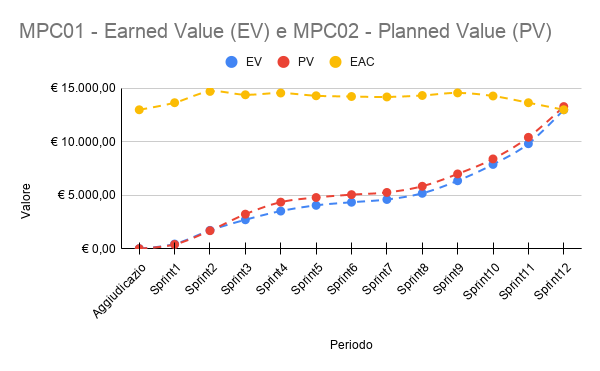
\includegraphics[width=0.8\textwidth]{../Assets/pdq/EV_PV.png}
    \caption{Andamento di Earned Value e Planned Value}
    \label{fig:ev_pv}
\end{figure}

\subsubsection*{RTB}
Dal grafico emerge un ritardo temporale crescente tra lo Sprint\textsuperscript{G} 2 e lo Sprint\textsuperscript{G} 4, dove l'Earned Value (EV) rimane costantemente sotto il Planned Value (PV) a causa di sottostime e sessioni d'esame. Tuttavia, lo Sprint\textsuperscript{G} 5 segna il punto di svolta: l'accelerazione dell'EV porta la curva a ricongiungersi quasi totalmente con il PV, dimostrando il successo delle contromisure del team. L'Estimate At Completion (EAC) si mantiene stabile sopra i 10.000€, confermando che, nonostante il ritardo iniziale, le previsioni di spesa finale restano coerenti con l'investimento. In conclusione, il progetto ha recuperato terreno e procede verso la Product Baseline con un budget sotto controllo.
\subsubsection*{PB}
Dal grafico esteso fino al termine della fase di Product Baseline, si osserva che tra lo Sprint 7 e lo Sprint 11 l'Earned Value (EV) si mantiene costantemente a un livello lievemente inferiore rispetto al Planned Value (PV), indicando un leggero ritardo strutturale durante le fasi centrali dello sviluppo. Tuttavia, a partire dallo Sprint 9 si registra una decisa accelerazione di entrambe le curve, a dimostrazione di un forte incremento del valore prodotto. L'Estimate At Completion (EAC), che all'inizio di questa fase si attestava su valori superiori ai 14.000€ per effetto delle inefficienze pregresse, mostra un trend progressivamente decrescente negli ultimi periodi. Nello Sprint 12, lo sforzo conclusivo del team permette il ricongiungimento tra EV e PV. 
\newpage

\subsection{Actual Cost e Estimate to Complete (MPC-03/07)}
\begin{figure}[h!]
    \centering
    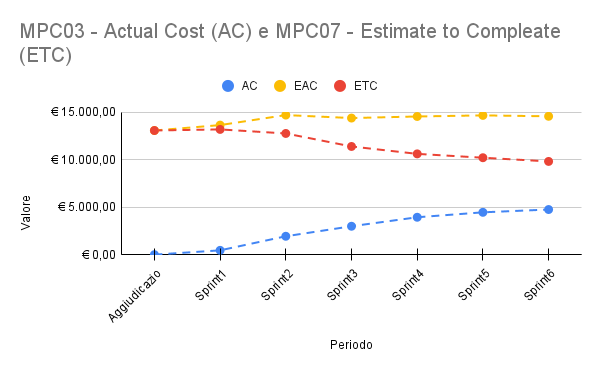
\includegraphics[width=0.8\textwidth]{../Assets/pdq/AC_ETC.png}
    \caption{Andamento di AC-ETC}
    \label{fig:ac_etc}
\end{figure}
\subsubsection*{RTB}
Dal grafico si evince un aumento costante dell'Actual Cost (AC) durante i primi 4 sprint\textsuperscript{G}, con un picco significativo nello Sprint\textsuperscript{G} 4 a causa di sottostime e sessioni d'esame. Tuttavia, a partire dallo Sprint\textsuperscript{G} 5, l'AC si stabilizza e mostra una leggera diminuzione, indicando un miglioramento nella gestione dei costi. L'Estimate to Complete (ETC) rimane relativamente stabile, suggerendo che le previsioni di completamento del progetto non sono state significativamente influenzate dalle variazioni dell'AC. In conclusione, nonostante le difficoltà iniziali, il team è riuscito a contenere i costi e a mantenere le stime di completamento sotto controllo.
\subsubsection*{PB}
Nella fase di Product Baseline, l'Actual Cost (AC) cresce in modo progressivo, registrando un'impennata a partire dallo Sprint\textsuperscript{G} 9 dovuta allo sforzo conclusivo di sviluppo e validazione. Simmetricamente, l'Estimate to Complete (ETC) decresce con regolarità fino ad azzerarsi nello Sprint\textsuperscript{G} 12, a conferma del completamento delle attività. Risulta positivo l'andamento dell'Estimate At Completion (EAC) che, dopo essersi mantenuto alto nella fase centrale, flette negli ultimi periodi per convergere in modo esatto con l'AC finale. In sintesi, il team ha gestito il carico conclusivo ottimizzando l'esecuzione e chiudendo il progetto in calo rispetto alle stime di picco.
\newpage

\subsection{Cost Performance Index e Schedule Performance Index (MPC-04/05)}
\begin{figure}[h!]
    \centering
    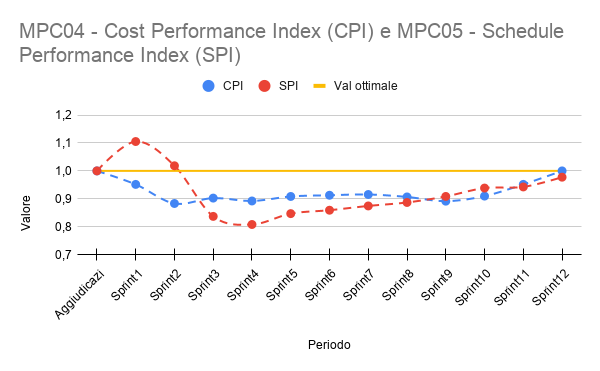
\includegraphics[width=0.8\textwidth]{../Assets/pdq/CPI_SPI.png}
    \caption{Andamento di CPI-SPI}
    \label{fig:cpi_spi}
\end{figure}
\subsubsection*{RTB}
Dal grafico emerge un trend iniziale negativo per entrambi gli indici, con il Cost Performance Index (CPI) che scende sotto 1 e il Schedule Performance Index (SPI) che si mantiene anch'esso sotto 1, indicando inefficienze sia nei costi che nella pianificazione. Tuttavia, a partire dallo Sprint\textsuperscript{G} 5, entrambi gli indici mostrano un miglioramento significativo: il CPI si avvicina a 1, suggerendo una gestione più efficiente dei costi, mentre lo SPI si avvicina anch'esso a 1, indicando un recupero nella pianificazione. In conclusione, nonostante le difficoltà iniziali, il team è riuscito a migliorare sia la performance dei costi che quella della pianificazione, avvicinandosi agli obiettivi prefissati.
\subsubsection*{PB}
Nella fase di Product Baseline, entrambi gli indici registrano un costante e progressivo miglioramento verso il valore ottimale. Lo Schedule Performance Index (SPI) cresce con regolarità a partire dallo Sprint\textsuperscript{G} 7, confermando il continuo riassorbimento del ritardo accumulato. Il Cost Performance Index (CPI), dopo essersi mantenuto stabile, sale in modo deciso negli ultimi sprint fino a raggiungere esattamente quota 1 nello Sprint\textsuperscript{G} 12. In sintesi, il team ha saputo correggere le inefficienze pregresse, chiudendo il progetto in perfetto allineamento con il budget e con un recupero quasi totale della pianificazione temporale.
\newpage

\subsection{Estimate At Completion (MPC-06)}
\begin{figure}[h!]
    \centering
    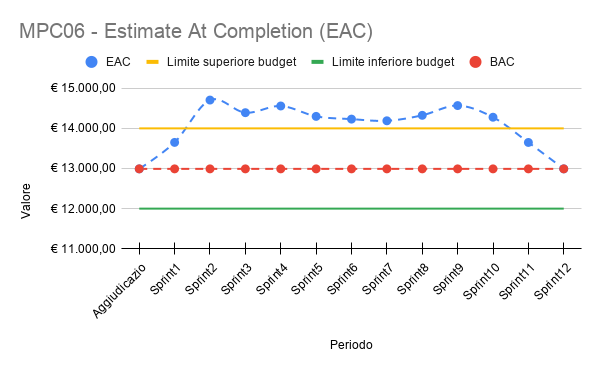
\includegraphics[width=0.8\textwidth]{../Assets/pdq/EAC.png}
    \caption{Andamento di EAC}
    \label{fig:eac}
\end{figure}
\subsubsection*{RTB}
Dal grafico si osserva un aumento costante dell'Estimate At Completion (EAC) durante i primi 4 sprint\textsuperscript{G}, con un picco significativo nello Sprint\textsuperscript{G} 4 a causa di sottostime e sessioni d'esame. Tuttavia, a partire dallo Sprint\textsuperscript{G} 5, l'EAC si stabilizza e mostra una leggera diminuzione, indicando che le contromisure adottate dal team hanno avuto successo nel contenere le previsioni di spesa finale. In conclusione, nonostante le difficoltà iniziali, il progetto sembra essere tornato su una traiettoria più sostenibile in termini di costi, con l'EAC che si mantiene sotto controllo.
\subsubsection*{PB}
Nella fase di Product Baseline, l'Estimate At Completion (EAC) permane oltre il limite superiore di budget fino allo Sprint\textsuperscript{G} 9, dove registra un ultimo picco. Successivamente, la curva mostra una rapida e decisa flessione: l'indicatore rientra nei parametri di tolleranza e, nello Sprint\textsuperscript{G} 12, converge in modo esatto con il Budget at Completion (BAC). In sintesi, il team ha compensato con successo le criticità della fase centrale, riportando i costi finali in perfetta linea con il preventivo originario.
\newpage

\subsection{Time Estimate At Completion (MPC-08)}
\begin{figure}[h!]
    \centering
    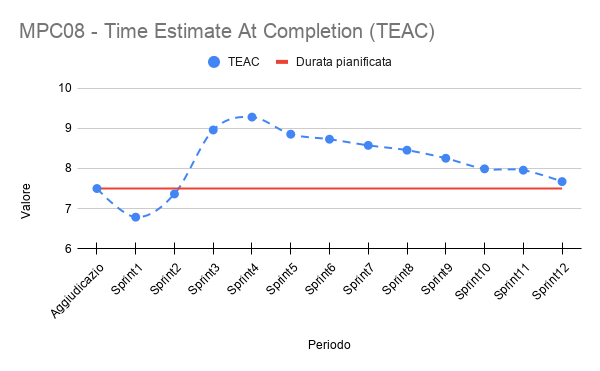
\includegraphics[width=0.8\textwidth]{../Assets/pdq/TEAC.png}
    \caption{Andamento di TEAC}
    \label{fig:teac}
\end{figure}
\subsubsection*{RTB}
Dal grafico si evince un aumento costante del Time Estimate At Completion (TEAC) durante i primi 4 sprint\textsuperscript{G}, con un picco significativo nello Sprint\textsuperscript{G} 4 a causa di sottostime e sessioni d'esame. Tuttavia, a partire dallo Sprint\textsuperscript{G} 5, il TEAC si stabilizza e mostra una leggera diminuzione, indicando che le contromisure adottate dal team hanno avuto successo nel contenere le previsioni di completamento del progetto. In conclusione, nonostante le difficoltà iniziali, il progetto sembra essere tornato su una traiettoria più sostenibile in termini di tempo, con il TEAC che si mantiene sotto controllo.
\subsubsection*{PB}
Nella fase di Product Baseline, il Time Estimate At Completion (TEAC) consolida in modo netto il proprio trend decrescente. Dallo Sprint\textsuperscript{G} 7 in avanti, l'indicatore si riduce con regolarità fino a quasi convergere con la durata pianificata durante lo Sprint\textsuperscript{G} 12. In sintesi, il team ha riassorbito gran parte del ritardo temporale accumulato nella fase iniziale, chiudendo il progetto con pochi ritardi.
\newpage

\subsection{Requirements Stability Index (MPC-09)}
\begin{figure}[h!]
    \centering
    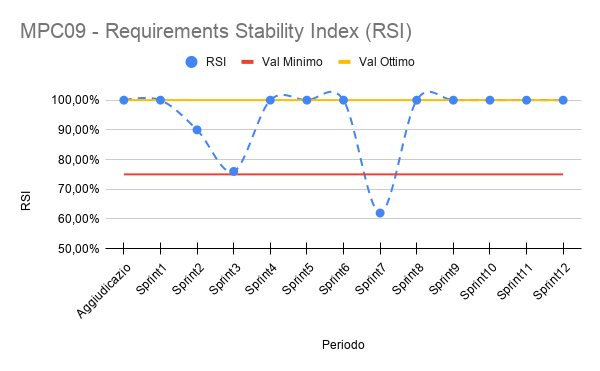
\includegraphics[width=0.8\textwidth]{../Assets/pdq/RSI.png}
    \caption{Andamento di RSI}
    \label{fig:rsi}
\end{figure}
\subsubsection*{RTB}
Dal grafico si osserva una stabilità iniziale del Requirements Stability Index (RSI) durante i primi 3 sprint\textsuperscript{G}, con valori vicini a 1, indicando che i requisiti sono rimasti relativamente stabili. Tuttavia, nello Sprint\textsuperscript{G} 4 si verifica un calo significativo dell'RSI, infatti in questo periodo sono stati rivisti e sistemati i requisiti. A partire dallo Sprint\textsuperscript{G} 5, l'RSI mostra un miglioramento e si avvicina nuovamente a 1, indicando che il team è riuscito a stabilizzare i requisiti e a ridurre le modifiche. In conclusione, nonostante le difficoltà iniziali, il progetto sembra essere tornato su una traiettoria più stabile in termini di requisiti.
\subsubsection*{PB} 
Nella fase di Product Baseline, l'indice RSI subisce un brusco calo nello Sprint\textsuperscript{G} 7, scendendo temporaneamente sotto la soglia minima a causa di un'importante revisione e rinegoziazione dei requisiti necessaria per l'avvio dell'ultima fase. Tuttavia, il riassetto si è rivelato efficace e definitivo: a partire dallo Sprint\textsuperscript{G} 8, l'indice si riporta immediatamente al valore ottimale del 100\%, mantenendo una stabilità assoluta fino al termine del progetto (Sprint\textsuperscript{G} 12). In sintesi, la baseline è stata consolidata con successo all'inizio del periodo, permettendo uno sviluppo conclusivo privo di ulteriori alterazioni ai requisiti.
\newpage

\subsection{Indice di Gulpease (MPC-10)}
\begin{figure}[h!]
    \centering
    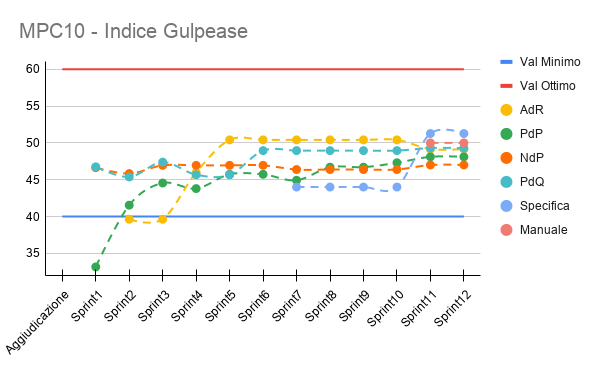
\includegraphics[width=0.8\textwidth]{../Assets/pdq/GULPEASE.png}
    \caption{Andamento della leggibilità dei documenti}
    \label{fig:gulpease_documenti}
\end{figure}
\subsubsection*{RTB}
Dal grafico si osserva un miglioramento costante dell'Indice di Gulpease durante i primi 4 sprint\textsuperscript{G}, con valori che si avvicinano a 50, indicando una discreta leggibilità della documentazione\textsuperscript{G}. Ad ogni sprint\textsuperscript{G} l'indice cresce, indicando che, nonostante l'aumento della dimensione della documentazione\textsuperscript{G}, la qualità continua a migliorare. Questo indica che il team è riuscito a migliorare la leggibilità dei documenti nonostante l'aumento del carico di lavoro. In conclusione, la qualità della documentazione\textsuperscript{G} è in costante miglioramento, con l'Indice di Gulpease che si avvicina a livelli ottimali.
\subsubsection*{PB}
Nella fase di Product Baseline, l'Indice di Gulpease conferma una solida stabilità per tutti i documenti\textsuperscript{G} preesistenti, che consolidano i propri valori ampiamente sopra la soglia minima, stabilizzandosi tra 45 e 50. Risulta particolarmente rilevante l'introduzione dei nuovi documenti tecnici: la Specifica, che dopo un lieve assestamento iniziale registra un netto miglioramento allo Sprint\textsuperscript{G} 11 superando quota 50, e il Manuale, che si attesta fin dal suo esordio sui medesimi livelli virtuosi. In sintesi, il team ha preservato e incrementato la leggibilità complessiva, gestendo con successo l'impatto derivante dalla stesura di nuova e complessa documentazione\textsuperscript{G}.
\newpage

\subsection{Indice di Gulpease Verbali (MPC-10)}
\begin{figure}[h!]
    \centering
    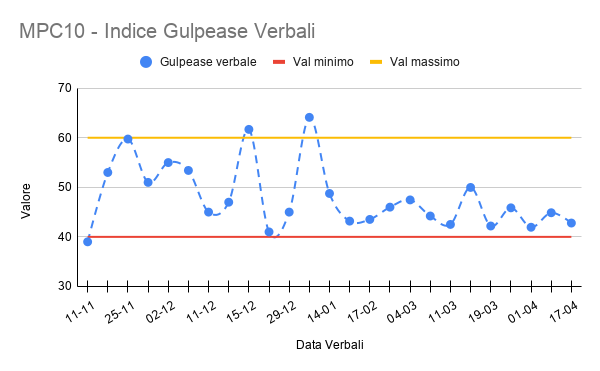
\includegraphics[width=0.8\textwidth]{../Assets/pdq/GULPEASE_VERBALE.png}
    \caption{Andamento della leggibilità dei verbali}
    \label{fig:gulpease_verbali}
\end{figure}
\subsubsection*{RTB}
Dal grafico si osserva che in linea di massima la stesura dei verbali mantiene un indice di Gulpease superiore a 40, indicando una buona leggibilità. In particolare si evidenzia una qualità di scrittura abbastanza regolare per tutti i verbali redatti durante il progetto, con un picco di leggibilità nello Sprint 5, dove l'indice supera i 60. Questo suggerisce che il team ha prestato particolare attenzione alla chiarezza e alla comprensibilità dei verbali in quel periodo. In conclusione, la qualità dei verbali è generalmente buona, con l'Indice di Gulpease che si mantiene a livelli accettabili.
\subsubsection*{PB}
Nella fase di Product Baseline (verbali successivi al 14-01), l'Indice di Gulpease mostra un andamento più lineare rispetto alla prima fase del progetto. Nonostante non si registrino più i picchi di eccellenza visti in precedenza (valori superiori a 60), l'indice si stabilizza in modo rassicurante all'interno del range di accettabilità, oscillando costantemente tra i 40 e i 50 punti. Questo andamento, seppur indicativo di testi più densi e tecnici, conferma che il team è riuscito a mantenere la leggibilità dei verbali sempre al di sopra della soglia minima critica per tutta la durata conclusiva del progetto.
\newpage
\subsection{Correttezza Ortografica (MPC-11)}
Monitoraggio degli errori ortografici presenti nella documentazione\textsuperscript{G} prodotta (Piano Qualifica, Analisi dei Requisiti\textsuperscript{G}, ecc.).
\begin{figure}[h!]
    \centering
    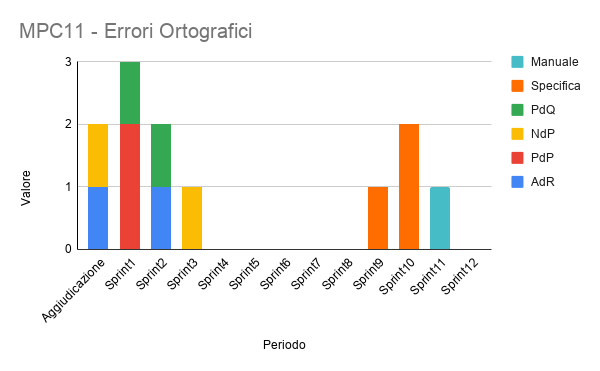
\includegraphics[width=0.8\textwidth]{../Assets/pdq/ORTOGRAFIA.png}
    \caption{Andamento degli errori ortografici presenti nei documenti}
    \label{fig:ortografia}
\end{figure}
\subsubsection*{RTB}
Dal grafico si osserva un miglioramento costante nella correttezza ortografica dei documenti prodotti durante il progetto. Nei primi 3 sprint\textsuperscript{G}, il numero di errori ortografici è contenuto ma è comunque superiore a zero. Il team ha preso fin da subito contromisure per ridurre gli errori. In conclusione, la correttezza ortografica è notevolmente migliorata nel corso del progetto, contribuendo a una comunicazione più chiara e professionale.
\subsubsection*{PB}
Nella fase di Product Baseline, la documentazione preesistente mantiene un livello di eccellenza, registrando la totale assenza di errori ortografici per l'intero periodo. Si rileva tuttavia la comparsa di alcune isolate imperfezioni tra lo Sprint\textsuperscript{G} 9 e lo Sprint\textsuperscript{G} 11: queste sono fisiologicamente legate alla prima stesura dei nuovi e corposi documenti tecnici (Specifica e Manuale). Grazie ai processi interni di verifica, tali sviste sono state prontamente individuate e sanate, permettendo al team di azzerare nuovamente il conteggio nello Sprint\textsuperscript{G} 12.
\newpage

\subsection{Quality metrics satisfied (MPC-14)}
\begin{figure}[h!]
    \centering
    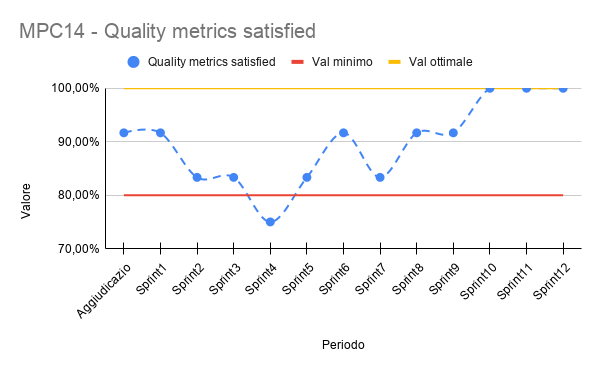
\includegraphics[width=0.8\textwidth]{../Assets/pdq/QMS.png}
    \caption{Andamento delle metriche soddisfatte}
    \label{fig:quality_metrics_satisfied}
\end{figure}
\subsubsection*{RTB}
Dal grafico si osserva un miglioramento abbastanza costante nel numero di metriche soddisfatte durante il progetto. Nei primi 3 sprint\textsuperscript{G}, il numero di metriche soddisfatte è relativamente basso, ma a partire dallo Sprint\textsuperscript{G} 4 si nota un aumento significativo, con un picco nello Sprint\textsuperscript{G} 5. Questo indica che il team ha adottato efficacemente le contromisure per migliorare la qualità del prodotto e del processo, portando a un maggior numero di metriche soddisfatte. In conclusione, il progetto ha mostrato un progresso significativo nel soddisfare le metriche di qualità, contribuendo al successo complessivo del progetto.
\subsubsection*{PB}
Nella fase di Product Baseline, la percentuale di metriche soddisfatte subisce una fisiologica flessione nello Sprint\textsuperscript{G} 7, pur mantenendosi saldamente al di sopra del valore minimo. Il team dimostra tuttavia una rapida capacità di riallineamento: la curva risale immediatamente, per poi compiere lo scatto decisivo nello Sprint\textsuperscript{G} 10, dove raggiunge il valore ottimale del 100\%. Tale traguardo di eccellenza viene mantenuto costante fino alla conclusione del progetto (Sprint\textsuperscript{G} 12). In sintesi, il gruppo ha saputo elevare e consolidare la qualità generale del lavoro, garantendo il pieno soddisfacimento di tutti i parametri previsti per il rilascio finale.
\newpage

\subsection{Sprint Goal Achievement (MPC-15)}
\begin{figure}[h!]
    \centering
    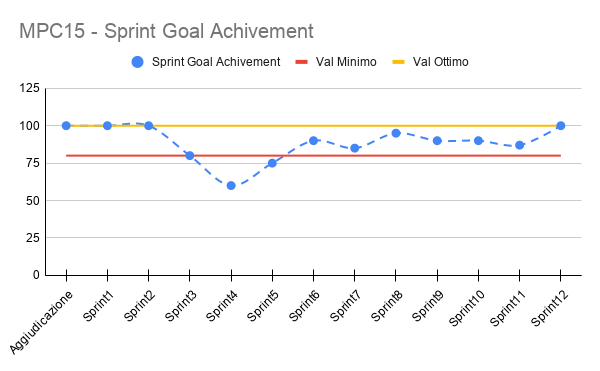
\includegraphics[width=0.8\textwidth]{../Assets/pdq/SGA.png}
    \caption{Andamento dello Sprint Goal Achievement}
    \label{fig:sprint_goal_achivement}
\end{figure}
\subsubsection*{RTB}
Il grafico evidenzia come negli sprint 4 e 5 il gruppo non abbia raggiunto il massimo degli obiettivi pianificati. Questo scostamento è riconducibile principalmente a due fattori: la sovrapposizione del periodo di sessione universitaria, che ha ridotto la disponibilità effettiva dei membri del team, e una sottostima iniziale del carico di lavoro necessario per completare le attività previste. Il gruppo ha preso atto di questa criticità e intende adottare una pianificazione più conservativa negli sprint futuri, tenendo conto dei periodi di minor disponibilità e calibrando il carico di lavoro in modo più realistico rispetto alle risorse effettivamente disponibili.
\subsubsection*{PB}
Nella fase di Product Baseline, l'indice di Sprint\textsuperscript{G} Goal Achievement si mantiene stabilmente al di sopra del valore minimo per l'intero periodo, confermando l'efficacia della pianificazione più conservativa adottata al termine della fase precedente. Tra lo Sprint\textsuperscript{G} 7 e lo Sprint\textsuperscript{G} 11, il raggiungimento degli obiettivi oscilla positivamente tra l'85\% e il 95\%, a dimostrazione di una gestione del carico di lavoro nettamente più realistica e calibrata. Nello Sprint\textsuperscript{G} 12 conclusivo, il team riesce a ultimare tutte le attività prefissate, riportando l'indicatore al valore ottimale del 100\%.


\newpage
%METRICHE DI PRODOTTO
\subsection{Requisiti Obbligatori Soddisfatti (MPD-01)}
\begin{figure}[h!]
    \centering
    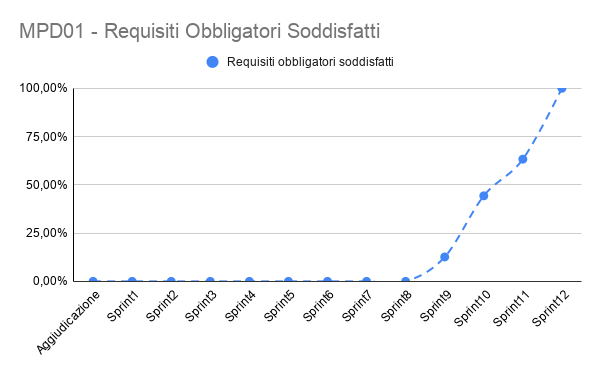
\includegraphics[width=0.8\textwidth]{../Assets/pdq/ROS.png}
    \caption{Andamento dei requisiti obbligatori soddisfatti}
    \label{fig:requisiti_obbligatori_soddisfatti}
\end{figure}
\subsubsection*{RTB}
Metrica non disponibile per la fase di RTB.
\subsubsection*{PB}
Coerentemente con l'avvio della fase di implementazione, l'indicatore mostra una rapida e costante ascesa a partire dallo Sprint\textsuperscript{G} 8. Capitalizzando il solido lavoro di progettazione della fase precedente, il team ha mantenuto un ritmo di sviluppo lineare ed efficace, arrivando a completare con successo il 100\% dei requisiti obbligatori nello Sprint\textsuperscript{G} 12 conclusivo.
\newpage

\subsection{Requisiti Desiderabili e Opzionali Soddisfatti (MPD-02/03)}
\begin{figure}[h!]
    \centering
    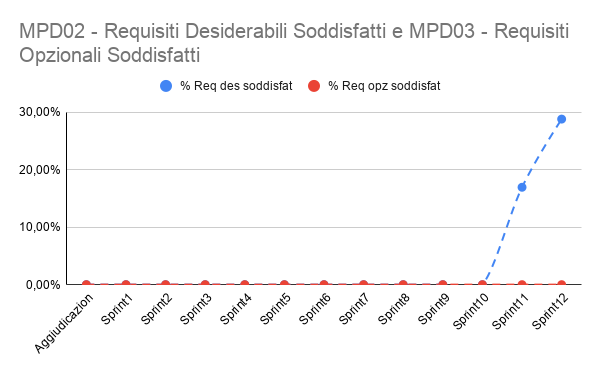
\includegraphics[width=0.8\textwidth]{../Assets/pdq/RDS_ROS.png}
    \caption{Andamento dei requisiti desiderabili e opzionali soddisfatti}
    \label{fig:requisiti_desiderabili_opzionali_soddisfatti}
\end{figure}
\subsubsection*{RTB}
Metrica non disponibile per la fase di RTB.
\subsubsection*{PB}
Nella fase di Product Baseline, il grafico evidenzia una rigorosa e matura gestione delle priorità di sviluppo. Fino allo Sprint\textsuperscript{G} 10, il team ha concentrato le proprie risorse esclusivamente sul nucleo essenziale del prodotto. Solo negli ultimi due periodi, avendo consolidato le funzionalità obbligatorie, è stato possibile riallocare lo sforzo sui requisiti desiderabili, riuscendo a soddisfarne circa il 30\% nello Sprint\textsuperscript{G} 12. I requisiti opzionali sono stati invece fisiologicamente esclusi per garantire il rigoroso rispetto delle tempistiche di consegna.
\newpage

\subsection{Condition Coverage (MPD-04)}
\begin{figure}[h!]
    \centering
    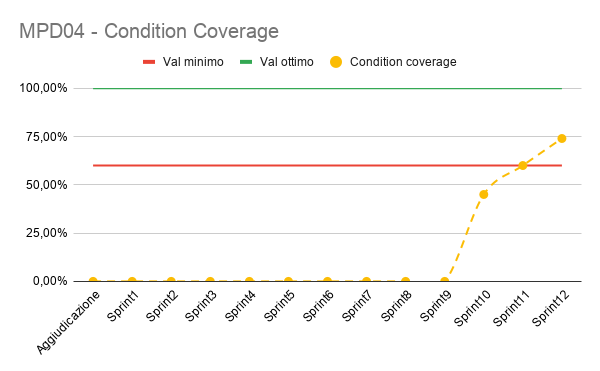
\includegraphics[width=0.8\textwidth]{../Assets/pdq/CV.png}
    \caption{Andamento della Condition Coverage}
    \label{fig:condition_coverage}
\end{figure}
\subsubsection*{RTB}
Metrica non disponibile per la fase di RTB.
\subsubsection*{PB}
L'andamento della Condition Coverage rispecchia in modo coerente le tempistiche di implementazione del codice sorgente. Essendo lo sviluppo effettivo dell'MVP iniziato nello Sprint\textsuperscript{G} 8, la stesura dei test automatici ha preso il via a partire dallo Sprint\textsuperscript{G} 9. Da questo momento, il grafico mostra una netta e continua ascesa, a dimostrazione di un sistematico e intenso sforzo di validazione da parte del team. Questa accelerazione ha permesso di superare la soglia minima di accettabilità (60\%) già durante lo Sprint\textsuperscript{G} 11, per poi consolidare il risultato chiudendo la fase di Product Baseline con una copertura del 75\% nello Sprint\textsuperscript{G} 12, garantendo così una solida affidabilità della base di codice consegnata.
\newpage

\subsection{Scan Response Time (MPD-05)}
\begin{figure}[h!]
    \centering
    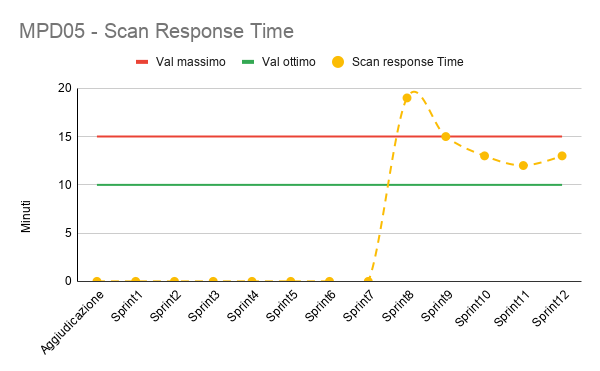
\includegraphics[width=0.8\textwidth]{../Assets/pdq/SRT.png}
    \caption{Andamento del Scan Response Time}
    \label{fig:scan_response_time}
\end{figure}
\subsubsection*{RTB}
Metrica non disponibile per la fase di RTB.
\subsubsection*{PB}
L'andamento dello Scan Response Time testimonia una gestione reattiva ed efficace delle performance del sistema. Con il rilascio del primo incremento software nello Sprint\textsuperscript{G} 8, la metrica ha registrato un picco iniziale (prossimo a 20), superando temporaneamente il limite massimo tollerato. Rilevata la criticità, il team è prontamente intervenuto con mirate operazioni di ottimizzazione e refactoring\textsuperscript{G}. Tali contromisure hanno permesso di ricondurre il tempo di risposta entro la soglia di accettabilità già nello Sprint\textsuperscript{G} 9. Negli sprint conclusivi l'indicatore si è progressivamente abbassato: la lieve fluttuazione registrata nello Sprint\textsuperscript{G} 12 risulta fisiologica all'integrazione delle ultime funzionalità, ma il valore si mantiene saldamente al di sotto del limite massimo, garantendo una reattività adeguata per il prodotto finale.
\newpage

\subsection{Facilità di utilizzo (MPD-06)}
\begin{figure}[h!]
    \centering
    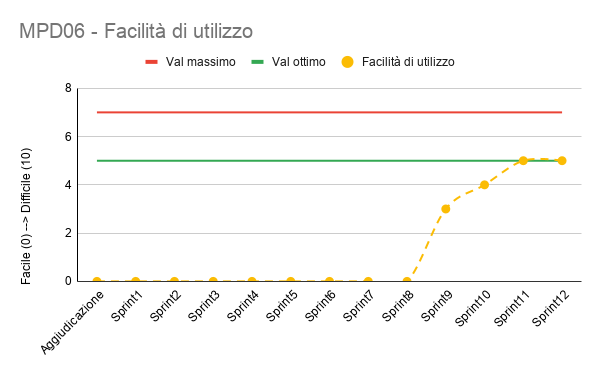
\includegraphics[width=0.8\textwidth]{../Assets/pdq/FU.png}
    \caption{Andamento della Facilità di utilizzo}
    \label{fig:facilita_di_utilizzo}
\end{figure}
\subsubsection*{RTB}
Metrica non disponibile per la fase di RTB.
\subsubsection*{PB}
L'indicatore della Facilità di Utilizzo registra i primi valori misurabili a partire dallo Sprint\textsuperscript{G} 9, in concomitanza con lo sviluppo e il rilascio delle interfacce utente. Il progressivo arricchimento delle funzionalità nei periodi successivi comporta una naturale crescita della metrica. Tuttavia, il team ha governato con successo l'aumento della complessità del sistema: l'indicatore si stabilizza in modo esatto sul valore ottimale negli Sprint\textsuperscript{G} 11 e 12, garantendo una navigabilità eccellente e mantenendosi sempre ampiamente al di sotto del limite massimo di tolleranza.
\newpage

\subsection{Tempo medio di apprendimento (MPD-07)}
\begin{figure}[h!]
    \centering
    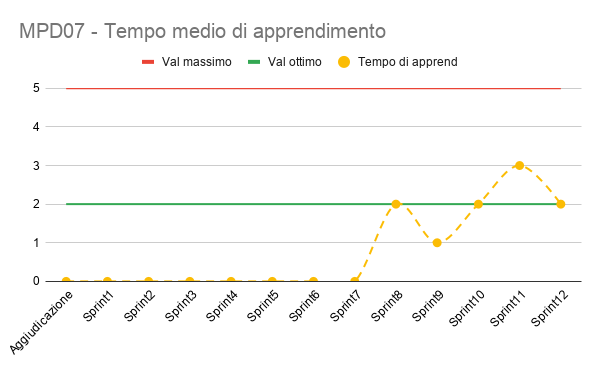
\includegraphics[width=0.8\textwidth]{../Assets/pdq/TMA.png}
    \caption{Andamento del Tempo medio di apprendimento}
    \label{fig:tempo_medio_di_apprendimento}
\end{figure}
\subsubsection*{RTB}
Metrica non disponibile per la fase di RTB.
\subsubsection*{PB}
L'andamento del Tempo Medio di Apprendimento riflette fedelmente le dinamiche dello sviluppo incrementale. Dopo un ingresso diretto sul valore ottimale nello Sprint\textsuperscript{G} 8, si osserva una fisiologica fluttuazione. Nello Sprint\textsuperscript{G} 11 l'indicatore registra un temporaneo picco (valore 3), in concomitanza con l'integrazione delle funzionalità più complesse che hanno richiesto un maggiore sforzo cognitivo iniziale da parte dell'utente. Tuttavia, le successive attività di raffinamento della User Experience\textsuperscript{G} hanno avuto pieno successo: nello Sprint\textsuperscript{G} 12 la metrica si consolida nuovamente sul valore ottimale (2), mantenendosi per l'intero periodo ampiamente al di sotto della soglia massima di tolleranza.
\newpage

\subsection{Linee per Metodo (MPD-09)}
\begin{figure}[h!]
    \centering
    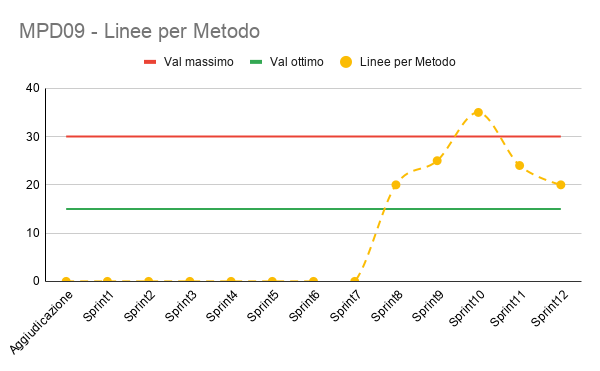
\includegraphics[width=0.8\textwidth]{../Assets/pdq/LPM.png}
    \caption{Andamento delle Linee per Metodo}
    \label{fig:linee_per_metodo}
\end{figure}
\subsubsection*{RTB}
Metrica non disponibile per la fase di RTB.
\subsubsection*{PB}
L'andamento della metrica Linee per Metodo riflette nitidamente le dinamiche della fase di codifica intensiva. A seguito dell'avvio dello sviluppo nello Sprint\textsuperscript{G} 8, l'indicatore subisce una rapida ascesa, culminando in un picco critico nello Sprint\textsuperscript{G} 10 (valore 35), dove sfora temporaneamente il limite massimo tollerato. Questo scostamento evidenzia un fisiologico accumulo di debito tecnico\textsuperscript{G} dovuto alle implementazioni più complesse. Avendo rilevato la criticità, il team è prontamente intervenuto negli Sprint\textsuperscript{G} 11 e 12 con mirate operazioni di refactoring\textsuperscript{G}, scomponendo le funzioni eccessivamente lunghe. Questa azione correttiva ha riportato con successo la metrica a quota 20, un valore ampiamente all'interno della zona di accettabilità, garantendo la manutenibilità del codice finale.
\newpage

\subsection{Parametri per Metodo (MPD-10)}
\begin{figure}[h!]
    \centering
    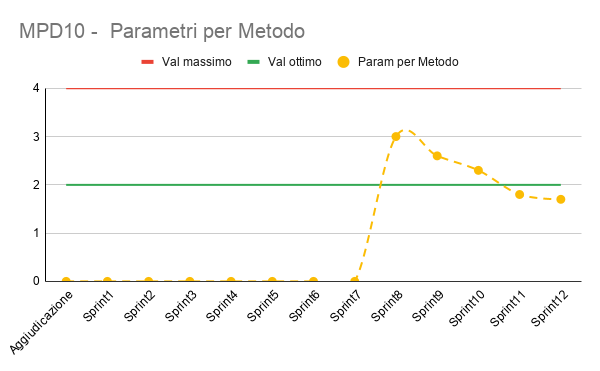
\includegraphics[width=0.8\textwidth]{../Assets/pdq/PPM.png}
    \caption{Andamento dei Parametri per Metodo}
    \label{fig:parametri_per_metodo}
\end{figure}
\subsubsection*{RTB}
Metrica non disponibile per la fase di RTB.
\subsubsection*{PB}
L'andamento dei Parametri per Metodo dimostra una progressiva e costante ottimizzazione dell'architettura software. Nelle prime fasi di codifica avviate nello Sprint\textsuperscript{G} 8, la metrica si attesta su un valore accettabile (3) ma ancora perfettibile. Nel corso degli sprint successivi, il team ha lavorato al miglioramento dell'incapsulamento\textsuperscript{G} dei dati e all'affinamento delle firme dei metodi, riducendo costantemente questo indicatore. Tale trend virtuoso si concretizza pienamente negli Sprint\textsuperscript{G} 11 e 12, dove il valore scende stabilmente al di sotto della soglia ottimale (2 parametri), confermando l'elevata pulizia e modularità della base di codice consegnata.
\newpage

\subsection{Attributi per Classe (MPD-11)}
\begin{figure}[h!]
    \centering
    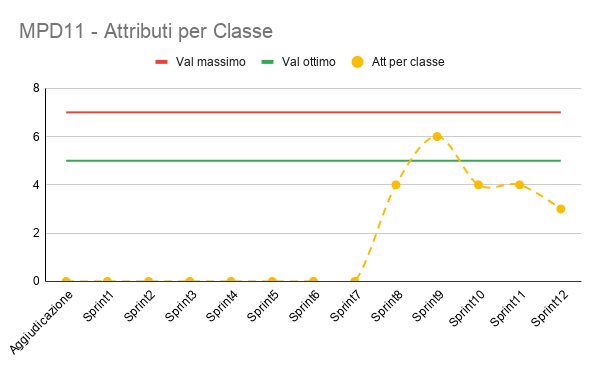
\includegraphics[width=0.8\textwidth]{../Assets/pdq/APC.png}
    \caption{Andamento degli Attributi per Classe}
    \label{fig:attributi_per_classe}
\end{figure}
\subsubsection*{RTB}
Metrica non disponibile per la fase di RTB.
\subsubsection*{PB}
L'andamento degli Attributi per Classe conferma un'attenta gestione della complessità strutturale del software. Avviato lo sviluppo nello Sprint\textsuperscript{G} 8 con un valore già ottimale (4), la metrica ha registrato un fisiologico innalzamento nello Sprint\textsuperscript{G} 9 (quota 6) dovuto all'integrazione di nuove logiche di stato. Pur superando temporaneamente la soglia ottimale, l'indicatore è stato mantenuto rigorosamente sotto il limite massimo di tolleranza. Le successive attività di refactoring\textsuperscript{G} hanno permesso di snellire le classi, riportando il valore al di sotto del target e chiudendo con un eccellente valore medio di 3 nello Sprint\textsuperscript{G} 12, a garanzia di un'alta coesione del codice prodotto.

% ====== INIZIATIVE DI AUTOMIGLIORAMENTO ======
%\newpage
%\section{Iniziative di automiglioramento}
%Il miglioramento continuo è essenziale per risolvere le criticità emerse durante gli sprint. Di seguito sono riportati i problemi principali riscontrati e le contromisure adottate.


\end{document}
